
\documentclass[11pt,compress,t,notes=noshow]{beamer}

\usepackage[english]{babel}
\usepackage{dsfont}
\newcommand\bmmax{2}
\usepackage{bm}
\usepackage{bbm}
\usepackage{verbatim}
\usepackage{amsmath}
\usepackage{amsfonts}
\usepackage{csquotes}
\usepackage{multirow}
\usepackage{longtable}
\usepackage{enumerate}
\usepackage[absolute,overlay]{textpos}
\usepackage{psfrag}
\usepackage{algorithm}
\usepackage{algorithmicx}
\usepackage{algpseudocode}
\usepackage{eqnarray}
\usepackage{multimedia}
\usepackage{media9}
\usepackage{arydshln}
\usepackage{tabularx}
\usepackage{placeins}
\usepackage{tikz}
\usepackage{setspace}
\usepackage{wrapfig}
\usepackage{tcolorbox}
\usepackage[export]{adjustbox}
\usepackage{siunitx}
\usetikzlibrary{shapes,arrows,automata,positioning,calc}
\tikzset{
  %Define standard arrow tip
  >=stealth',
  %Define style for boxes
  punkt/.style={
    rectangle,
    rounded corners,
    draw=black, very thick,
    text width=6.5em,
    minimum height=2em,
    text centered},
  % Define arrow style
  pil/.style={
    ->,
    thick,
    shorten <=2pt,
    shorten >=2pt,}
}
\usepackage{subfig}

%new environments

\newenvironment{vbframe}  %frame with breaks and verbatim
{
 \begin{frame}[containsverbatim,allowframebreaks]
}
{
\end{frame}
}

\newenvironment{vframe}  %frame with verbatim without breaks (to avoid numbering one slided frames)
{
 \begin{frame}[containsverbatim]
}
{
\end{frame}
}

\newenvironment{blocki}[1]   % itemize block
{
 \begin{block}{#1}\begin{itemize}
}
{
\end{itemize}\end{block}
}

\newenvironment{fragileframe}[2]{  %fragile frame with framebreaks
\begin{frame}[allowframebreaks, fragile, environment = fragileframe]
\frametitle{#1}
#2}
{\end{frame}}


\newcommand{\myframe}[2]{  %short for frame with framebreaks
\begin{frame}[allowframebreaks]
\frametitle{#1}
#2
\end{frame}}

\newcommand{\remark}[1]{
  \textbf{Remark:} #1
}

%%%%%%%%%%%%%%%%%%%%%%%%%%%%%%%%%%%%%%%%%%%%%%%%%%%%%%%%%%%%%%%%%%%%%%%%%%%%%%%

% basic latex stuff
\newcommand{\pkg}[1]{{\fontseries{b}\selectfont #1}} %fontstyle for R packages
\newcommand{\lz}{\vspace{0.5cm}} %vertical space
\newcommand{\dlz}{\vspace{1cm}} %double vertical space
\newcommand{\oneliner}[1] % Oneliner for important statements
{\begin{block}{}\begin{center}\begin{Large}#1\end{Large}\end{center}\end{block}}


%\usetheme{lmu-lecture}
\usepackage{../style/lmu-lecture}

\let\code=\texttt
\let\proglang=\textsf

\setkeys{Gin}{width=0.9\textwidth}



\title{Deep Learning}
\author{David Rügamer}
\institute{Department of Statistics -- LMU Munich}
\date{Winter Semester 2021}

\setbeamertemplate{frametitle}{\expandafter\uppercase\expandafter\insertframetitle}

%\begin{document}
%\sloppy
%\end{document}


\input{../../latex-math/basic-math}
\input{../../latex-math/basic-ml}
\input{../../latex-math/ml-nn}

\begin{document}

\lecturechapter{1}{Feedforward Neural Networks}
\lecture{Deep Learning}


%%%%%%%%%%%%%%%%%%%%%%%%%%%%%%%%%%%%%%%%%%%%%%%%%%%%%%%%%%%%%%%%%%

\begin{frame}
\frametitle{Lecture outline}
\tableofcontents
\end{frame}

\begin{frame} {Motivation}
  \begin{itemize}
    \vspace{2mm}
    \item We have a nice graphical way of representing simple functions/models like logistic regression. Why is that useful?
    \vspace{5mm}
    \item It is useful because this visual metaphor allows us to use such individual neurons as building blocks of considerably more complicated functions.
    \vspace{5mm}
    \item Therefore, networks of neurons can represent extremely complex hypothesis spaces.
    \vspace{5mm}
    \item Most importantly, it allows us to define the \enquote{right} kinds of hypothesis spaces to learn functions that are more common in our universe in a data-efficient way (see Lin, Tegmark et al. 2016).
  \end{itemize}
\end{frame}

\begin{frame} {Motivation}
  \begin{itemize}
    \item \small{But why do we need more complicated functions? Is logistic regression not enough?}
    \item \small{Because a single neuron is restricted to learning only linear decision boundaries, its performance on the task below will be quite poor. }
    \begin{figure}
    \centering
      \scalebox{0.25}{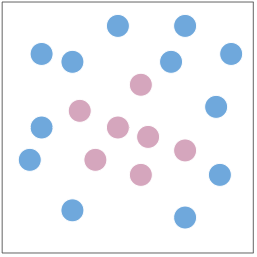
\includegraphics{plots/cartesian.png}}
  \end{figure}
    \item \small{However, if the original features are transformed (for example from Cartesian to polar coord.), the neuron can easily separate the classes.}
    \begin{figure}
    \centering
      \scalebox{0.25}{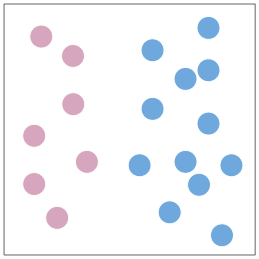
\includegraphics{plots/polar.png}}
  \end{figure}
  \end{itemize}
\end{frame}

\begin{frame} {Motivation}
  \small{Instead of classifying the data in the original representation, ...}
    \begin{figure}
    \centering
      \scalebox{1}{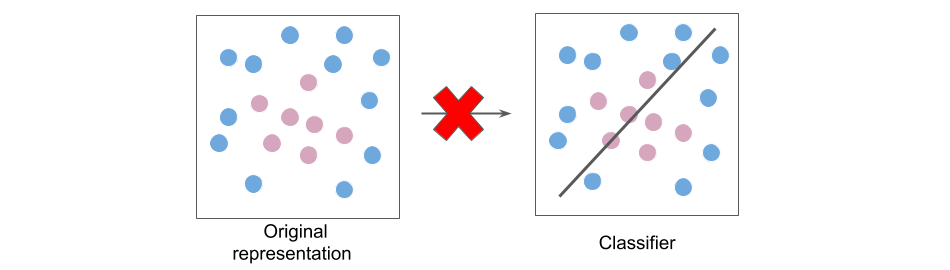
\includegraphics{plots/repold_f.png}}
  \end{figure}
\end{frame}

\begin{frame} {Motivation}
   \small{we classify it in the new feature space.}
  \begin{figure}
    \centering
      \scalebox{1}{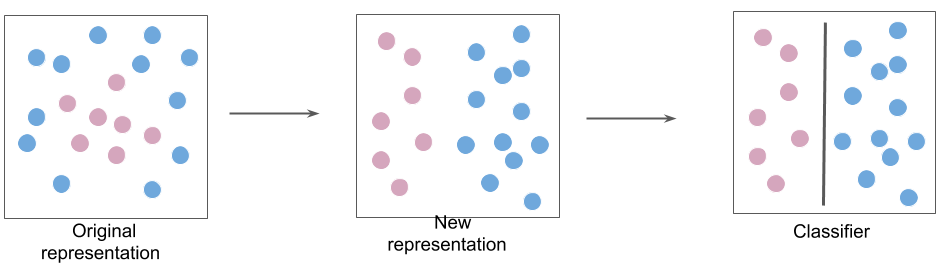
\includegraphics{plots/repnew_f.png}}
  \end{figure}
\end{frame}

\begin{frame} {Motivation}
   \small{we classify it in the new feature space.}
  \begin{figure}
    \centering
      \scalebox{1}{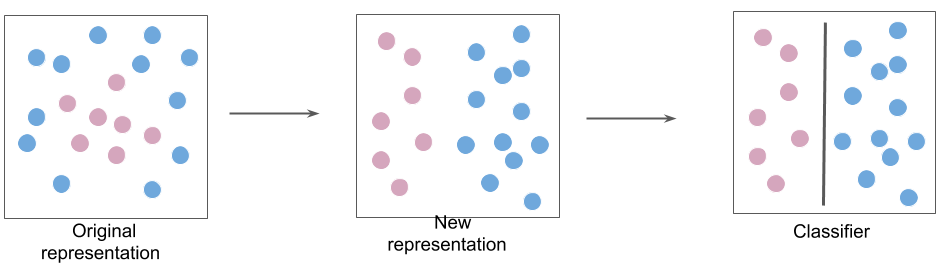
\includegraphics{plots/repnew_f.png}}
  \end{figure}
  \small{Analogously, }
  \begin{figure}
    \centering
      \scalebox{0.75}{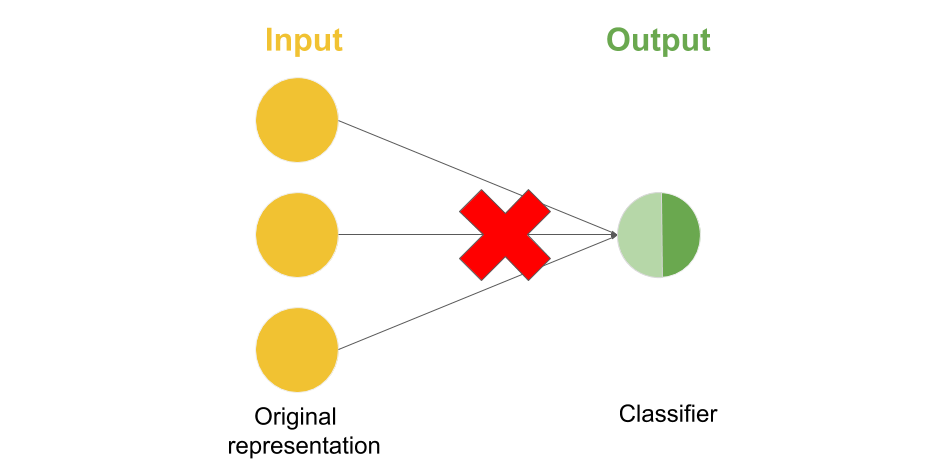
\includegraphics{plots/oldrep_n_f.png}}
  \end{figure}
\end{frame}

\begin{frame} {Motivation}
   \small{we classify it in the new feature space.}
  \begin{figure}
    \centering
      \scalebox{1}{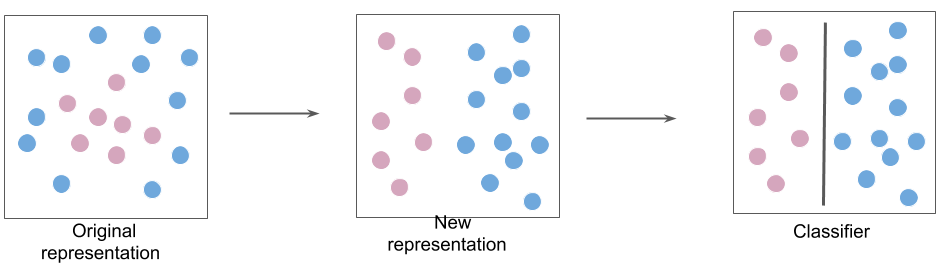
\includegraphics{plots/repnew_f.png}}
  \end{figure}
  \small{Analogously, }
  \begin{figure}
    \centering
      \scalebox{0.75}{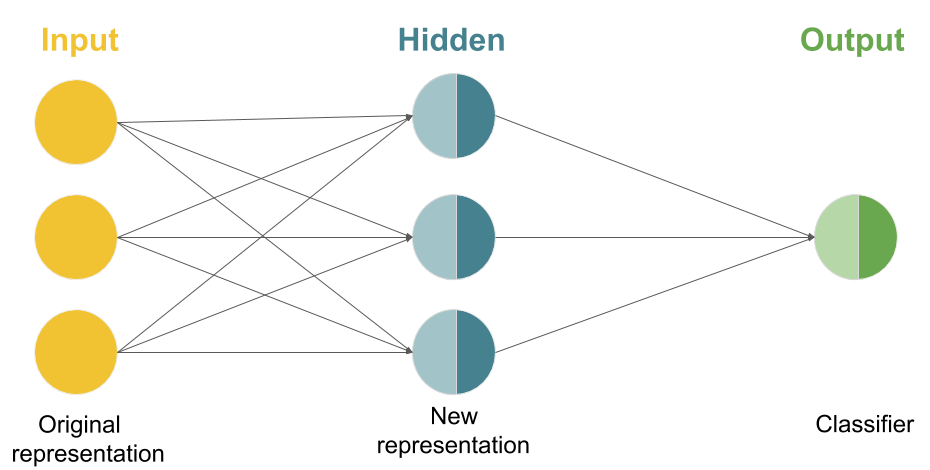
\includegraphics{plots/newrep_n_f.png}}
  \end{figure}
\end{frame}

\begin{frame} {Representation Learning}
  \begin{itemize}
    \vspace{5mm}
    \item Therefore, it is \textit{very} critical to feed a classifier the \enquote{right} features in order for it to perform well.
    \vspace{7mm}
    \item Before deep learning (DL) took off, features for tasks like machine vision and speech recognition were \enquote{hand-designed} by domain experts. This step of the machine learning pipeline is called \textbf{feature engineering}.
    \vspace{7mm}
    \item The single biggest reason DL is so important is that it automates feature engineering. This is called \textbf{representation learning}.
  \end{itemize}
\end{frame}



% \begin{vbframe} {Representation Learning}
%   \begin{itemize}
%     \item To understand how feature engineering can be automated, let us consider networks with a single hidden layer first: 
%    \begin{figure}
%         \centering
%           \scalebox{0.7}{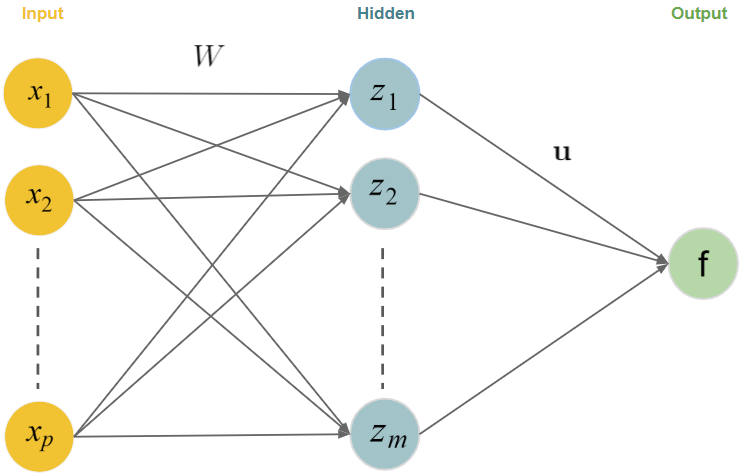
\includegraphics{plots/neuralnet2_new.png}}
%           \caption{Structure of a single hidden layer, feed-forward neural network for regression or binary classification problems (bias term omitted). Such a network is sometimes referred to as a \enquote{shallow neural network}.}
%       \end{figure}
% 
%     \framebreak 
% 
%     \item We represent the new features as intermediate neurons called \textbf{hidden neurons}.
%     \vspace{3mm}
%     \item Different weights correspond to different features and \enquote{good} weights are learned from the data in an end-to-end fashion.
%     \vspace{3mm}
%     \item The final neuron will now be referred to as the \textbf{output neuron}.
%     \vspace{3mm}
%     \item The classifier can learn a linear decision boundary in the transformed space (a similar argument applies to regression).
%     \vspace{3mm}
%     \item It is very important to note that both the intermediate feature transformations and the final classifier are learned from data simultaneously.
%   \end{itemize}
% \end{vbframe}


\section{Single Hidden Layer Networks for Regression and Binary Classification}

\begin{vbframe} {Single Hidden Layer Networks}

  \begin{itemize}
    \item The input $\xv$ is a column vector with dimensions $p \times 1$. 
    \item $\Wmat$ is a weight matrix with dimensions $p \times m$:
    $$
    \Wmat =
     \begin{pmatrix}
      w_{1,1} & w_{1,2} & \cdots & w_{1,m} \\
      w_{2,1} & w_{2,2} & \cdots & w_{2,m} \\
      \vdots  & \vdots  & \ddots & \vdots  \\
      w_{p,1} & w_{p,2} & \cdots & w_{p,m}
     \end{pmatrix}
    $$
    \item For example, to obtain $z_1$, we pick the first column of $W$:
    $$
    \Wmat_1 =
     \begin{pmatrix}
      w_{1,1} \\
      w_{2,1} \\
      \vdots  \\
      w_{p,1}
     \end{pmatrix}
    $$
    and compute $z_1 = \sigma(W_1^\top \xv + b_1)$, where $b_1$ is the bias of the first hidden neuron and $\sigma: \R \to \R$ is an activation function. 
  \end{itemize}
\end{vbframe}

\begin{vbframe}{Single Hidden Layer Networks: Notation}
  \textbf{General notation}:
  \begin{itemize}
    \vspace{4mm}
    \item The network has $m$ hidden neurons $z_1, \dots, z_m$ with
    $$ z_j = \sigma(\Wmat_j^\top \xv + b_j)$$
    \vspace{-0.5cm}
    \begin{itemize}
    \item $z_{in,j}  = \Wmat_j^\top \xv + b_j$
    \vspace{2mm}
    \item $z_{out,j} = \sigma(z_{in,j}) = \sigma(\Wmat_j^\top \xv + b_j)$
    \end{itemize}
    \vspace{4mm}
    for $j \in \{1,\ldots,m\}$.
    \vspace{4mm}

    \framebreak 

    \item Vectorized notation:
      \begin{itemize}
        \item $ \hidz_{in} = (z_{in,1}, \dots, z_{in,m})^\top = \Wmat^\top \xv + \biasb$ \\ (Note: $\Wmat^\top \xv$ = $(\xv^\top \Wmat)^\top$)
        \item $ \hidz = \hidz_{out} = \sigma(\hidz_{in}) = \sigma(\Wmat^\top \xv + \biasb)$, where the (hidden layer) activation function $\sigma$ is applied element-wise to $\hidz_{in}$.  
      \end{itemize}
      \item Bias term:         
      \begin{itemize}
        \item We sometimes omit the bias term by adding a constant feature to the input $\tilde{\xv} = (1, x_1, ..., x_p)$ and by adding the bias term to the weight matrix 
        $$
          \tilde{\Wmat} = (\biasb, \Wmat_1, ..., \Wmat_p). 
        $$ 
        \item \textbf{Note}: For simplification purposes, we will not explicitly represent the bias term graphically in the following. However, the above \enquote{trick} makes it straightforward to represent it graphically. 
      \end{itemize}
    \end{itemize}



\framebreak
  \textbf{General notation}:
  \begin{itemize}
    \vspace{4mm}
    \item For regression or binary classification: one output unit $f$ where
      \begin{itemize}
        \item $f_{in} = \wtu^\top \hidz + c$ , i.e. a linear combination of derived features plus the bias term $c$ of the output neuron, and
        \vspace{2mm}
        \item $f(\xv)= f_{out} = \tau(f_{in}) = \tau(\wtu^\top \hidz + c)$ , where $\tau$ is the output activation function.
      \end{itemize}
    \item For regression $\tau$ is the identity function.
    \item For binary classification, $\tau$ is a sigmoid function.
    \item \textbf{Note}: The purpose of the hidden-layer activation function $\sigma$ is to introduce non-linearities so that the network is able to learn complex functions whereas the purpose of $\tau$ is merely to get the final score on the same scale as the target.
  \end{itemize}

\framebreak 

  \textbf{General notation: Multiple inputs}
  \begin{itemize}
    \item It is possible to feed multiple inputs to a neural network simultaneously.
    \vspace{2mm}
    \item The inputs $\xi$, for $i \in \nset$, are arranged as rows in the \textbf{design matrix} $\Xmat$.
    \begin{itemize}
      \item $\Xmat$ is a ($n \times p$)-matrix.
    \end{itemize}
    \vspace{2mm}
    \item The weighted sum in the hidden layer is now computed as $\Xmat\Wmat + \bm{B}$, where,
      \begin{itemize}
        \item $\Wmat$, as usual, is a ($p \times m$) matrix, and,
        \vspace{2mm}
        \item $\bm{B}$ is a ($n \times m$) matrix containing the bias vector $\biasb$ (duplicated) as the rows of the matrix.
      \end{itemize}
    \vspace{2mm}
    \item The \textit{matrix} of hidden activations $\bm{Z} = \sigma(\Xmat\Wmat + \bm{B})$
    \begin{itemize}
      \item $\bm{Z}$ is a ($n \times m$) matrix.
    \end{itemize}
  \end{itemize}

\framebreak
  % \textbf{General notation: Batch processing}
  \begin{itemize}
    \vspace{15mm}
    \item The final output of the network, which contains a prediction for each input, is $\tau(\bm{Z}\wtu + \bm{C})$, where
      \begin{itemize}
        \vspace{2mm}
        \item $\wtu$ is the vector of weights of the output neuron, and,
        \vspace{2mm}
        \item $\bm{C}$ is a ($n \times 1$) matrix whose elements are the (scalar) bias $c$ of the output neuron.
      \end{itemize}
  \end{itemize}
\end{vbframe}

\begin{frame} {Single Hidden Layer Networks: Example}
  \begin{itemize}
    \item Weights (and biases) of the network.
  \begin{figure}
    \centering
      \only<1>{\scalebox{1}{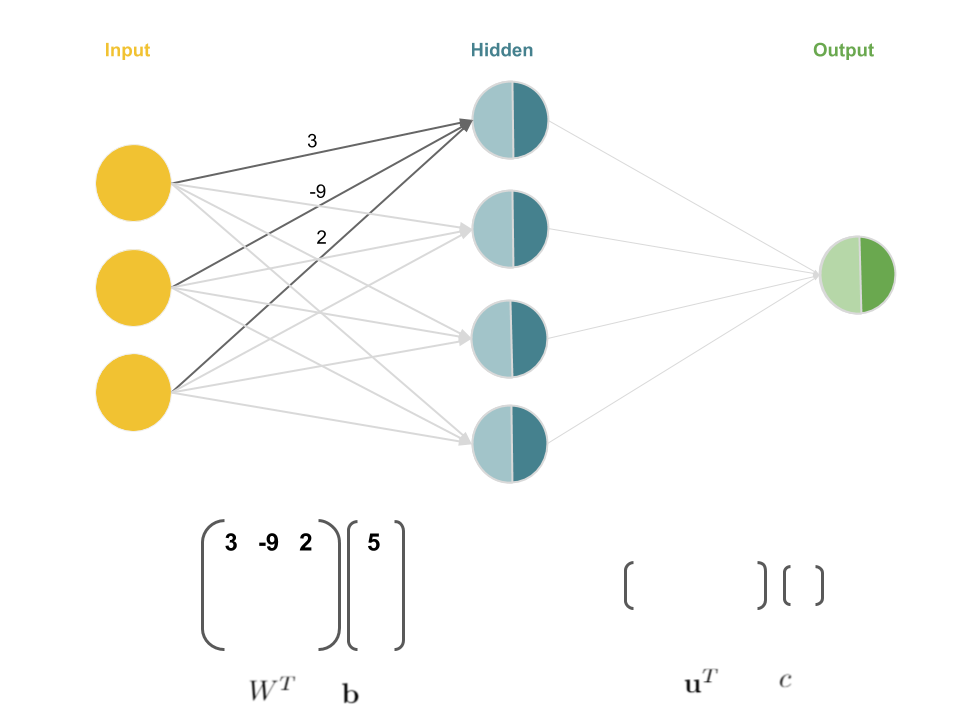
\includegraphics{plots/sinlay_one.png}}}
      \only<2>{\scalebox{1}{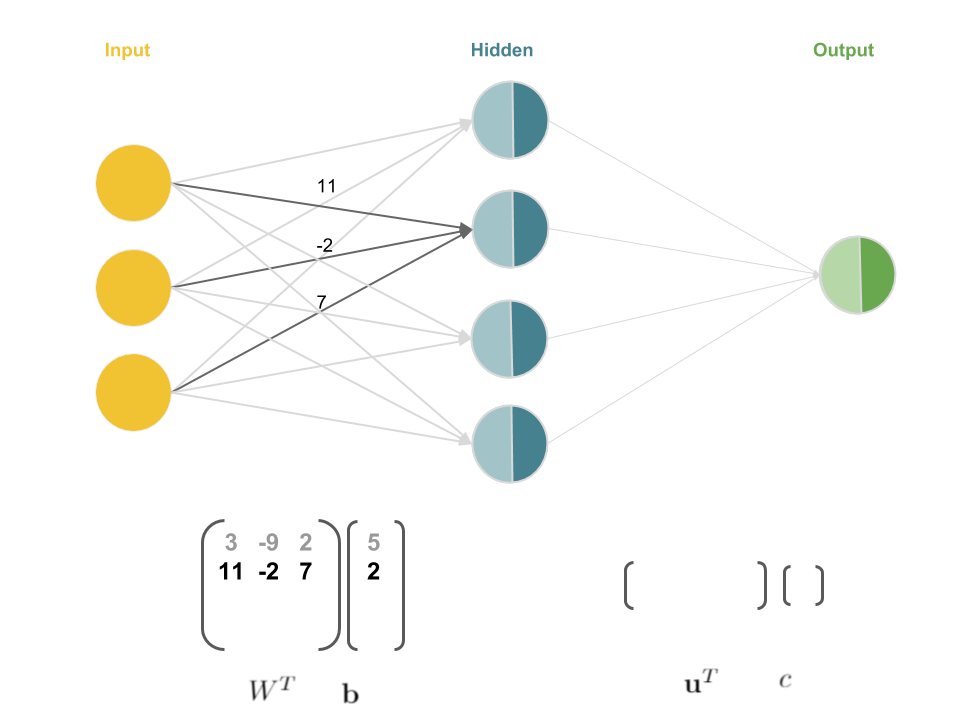
\includegraphics{plots/sinlay_two.png}}}
      \only<3>{\scalebox{1}{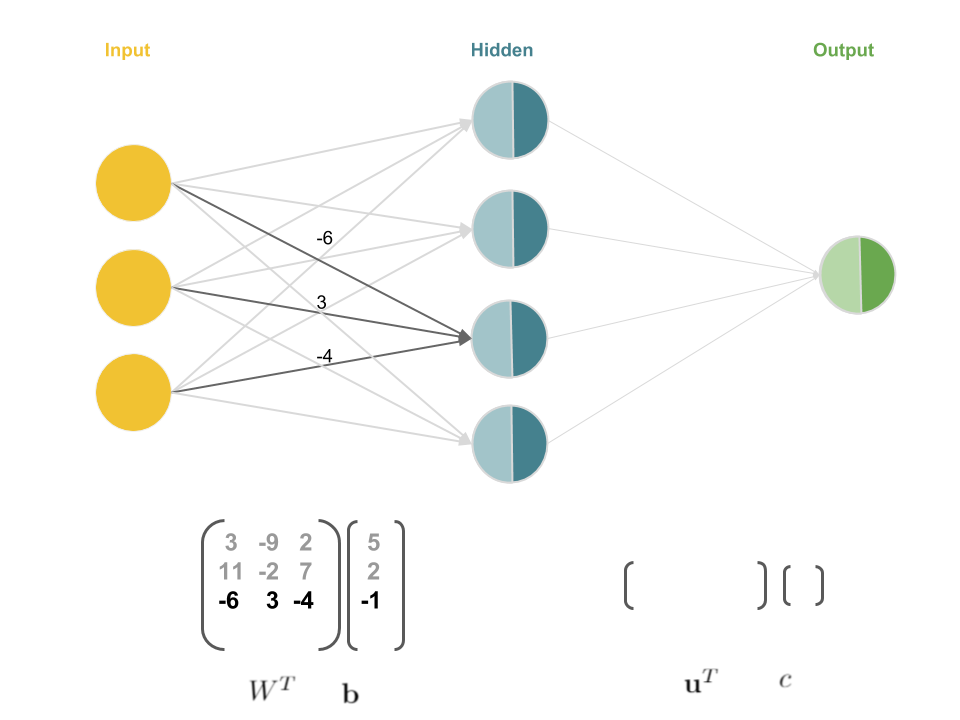
\includegraphics{plots/sinlay_three.png}}}
      \only<4>{\scalebox{1}{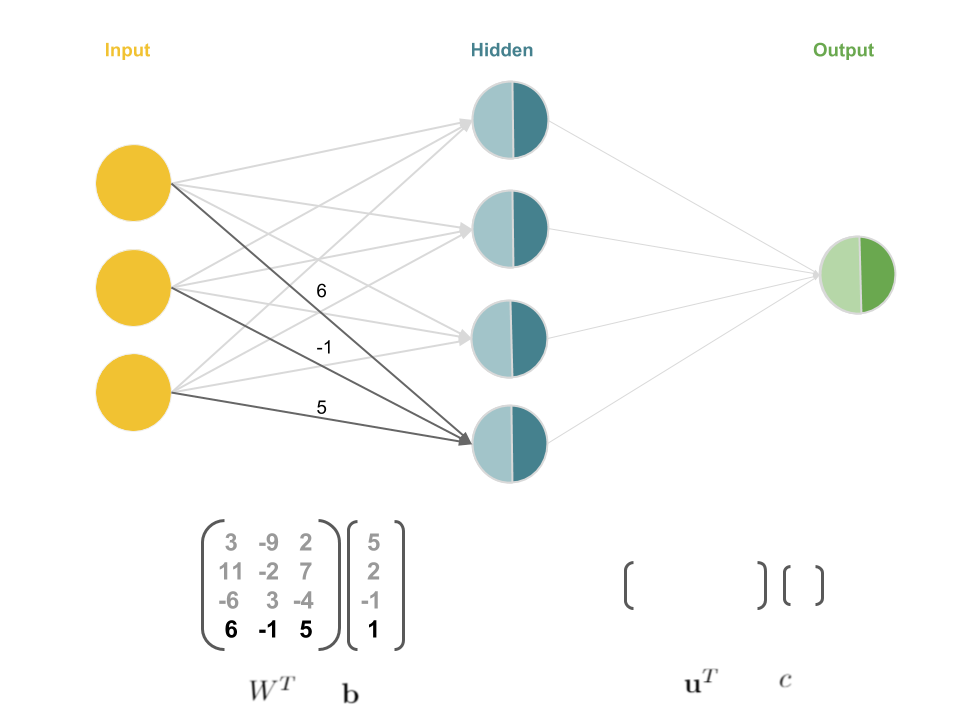
\includegraphics{plots/sinlay_four.png}}}
      \only<5>{\scalebox{1}{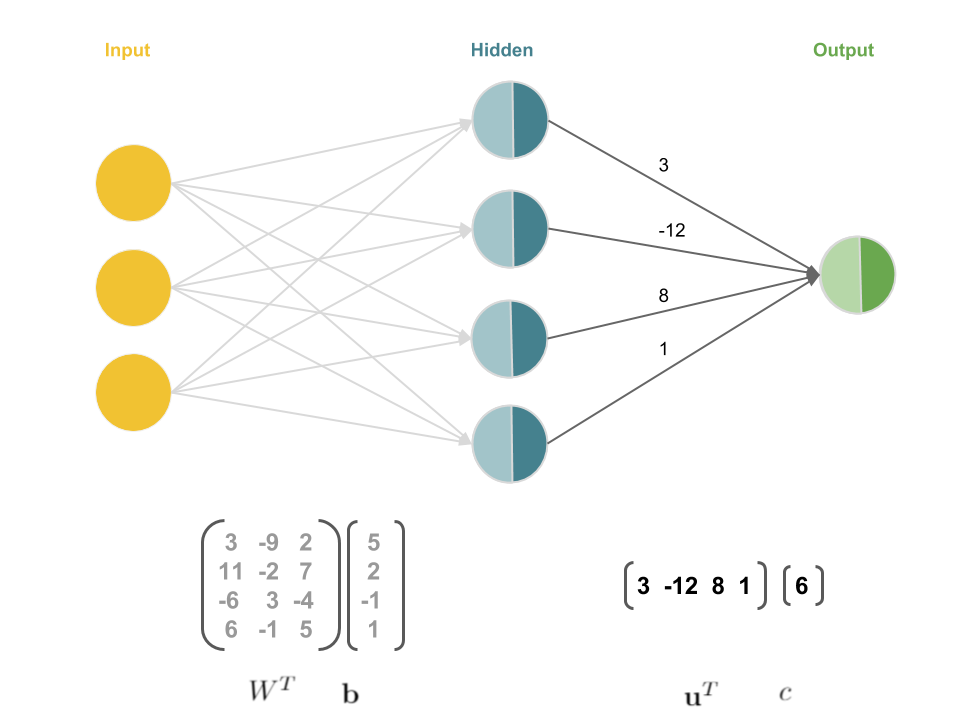
\includegraphics{plots/sinlay_five.png}}}
      \only<6>{\scalebox{1}{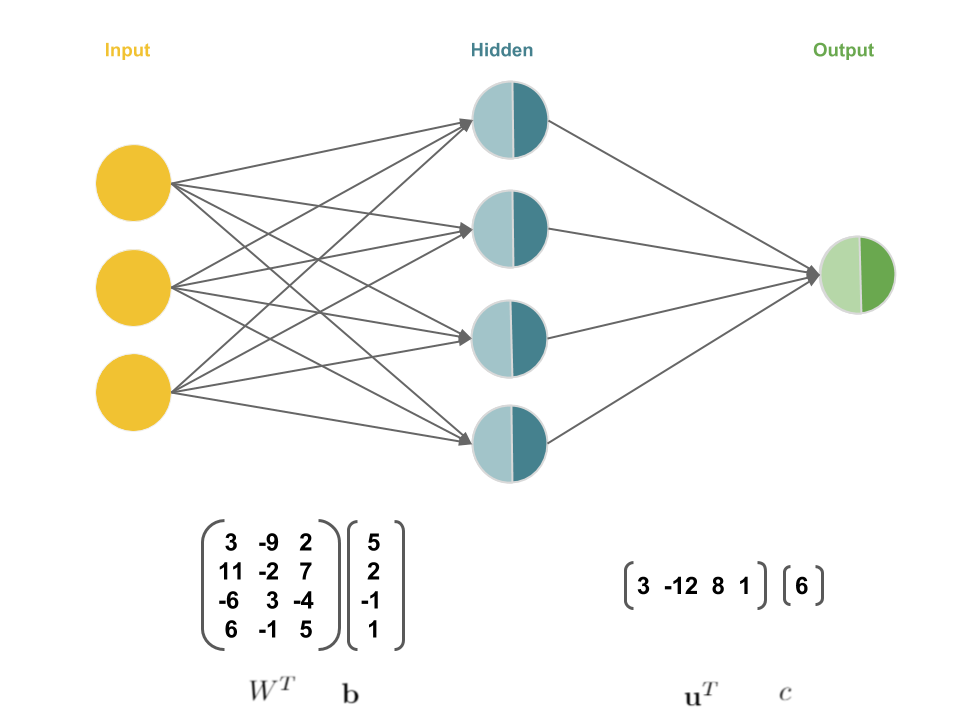
\includegraphics{plots/sinlay_six.png}}}
  \end{figure}
  \begin{figure}
    \centering
  \end{figure}
  \end{itemize}
\end{frame}

\begin{frame} {Single Hidden Layer Networks: Example}
  
  \small{Forward pass through the shallow neural network.}
  \begin{figure}
    \centering
    \only<1>{\scalebox{1}{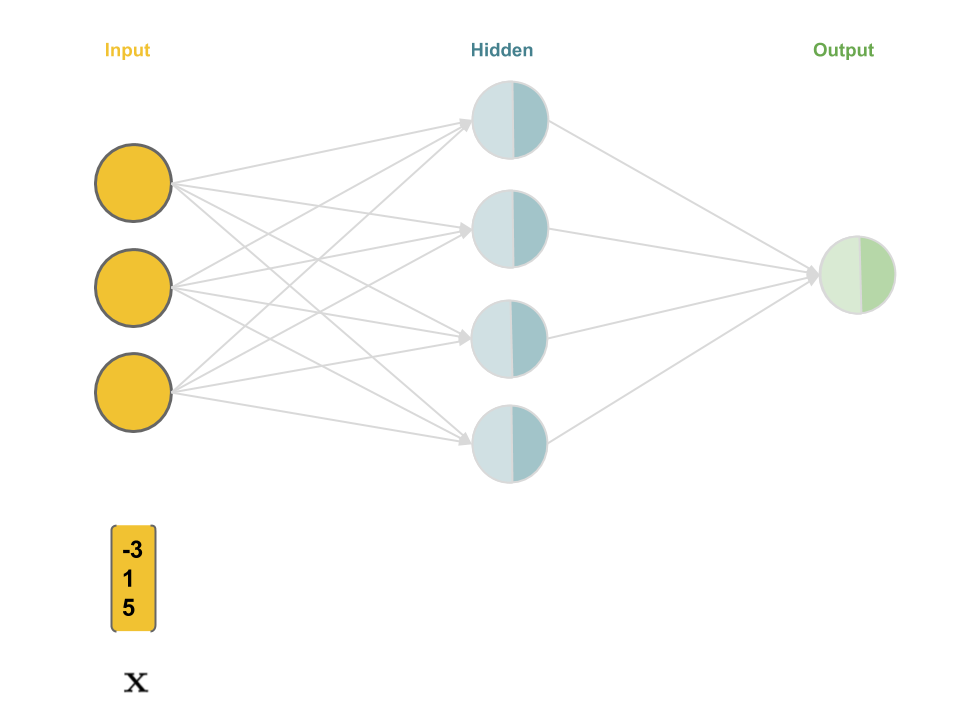
\includegraphics{plots/sinlay_seven.png}}}
    \only<2>{\scalebox{1}{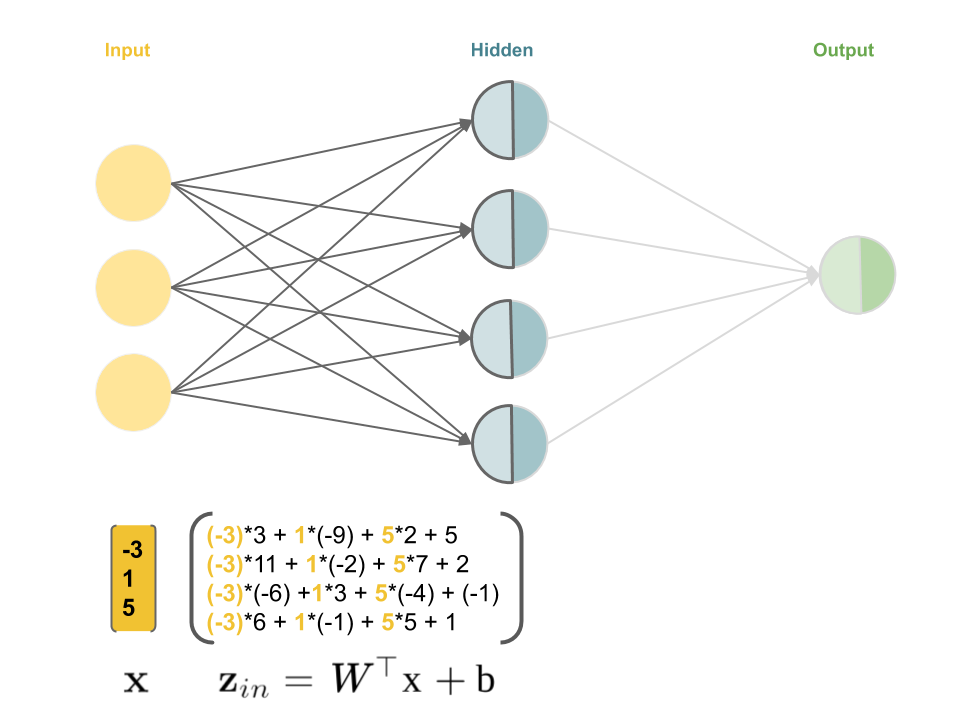
\includegraphics{plots/sinlay_eight.png}}}
    \only<3>{\scalebox{1}{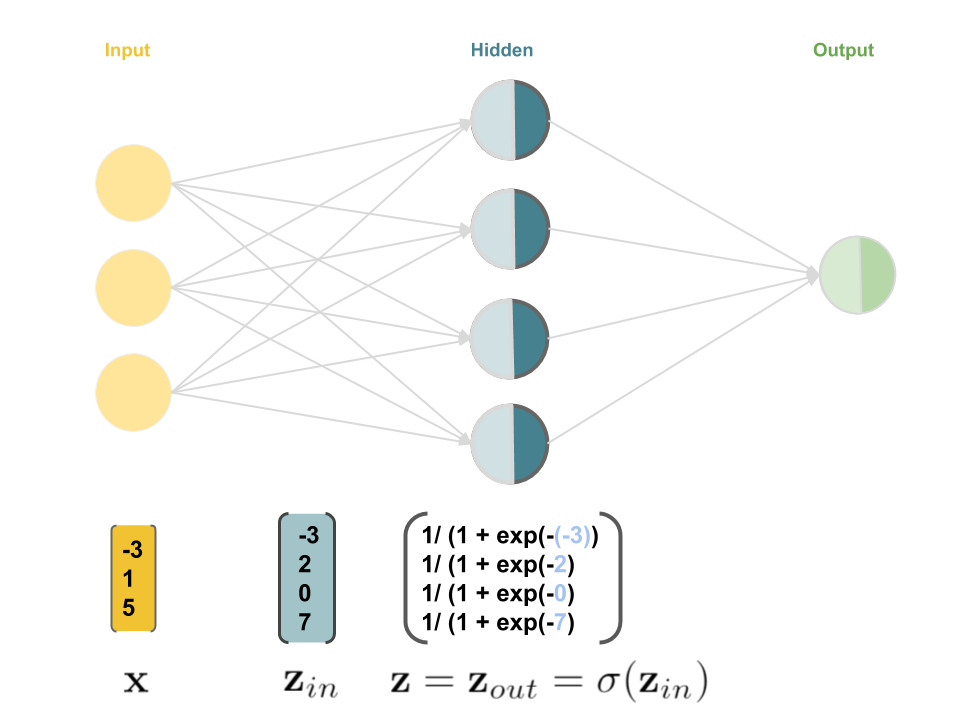
\includegraphics{plots/sinlay_nine.png}}}
    \only<4>{\scalebox{1}{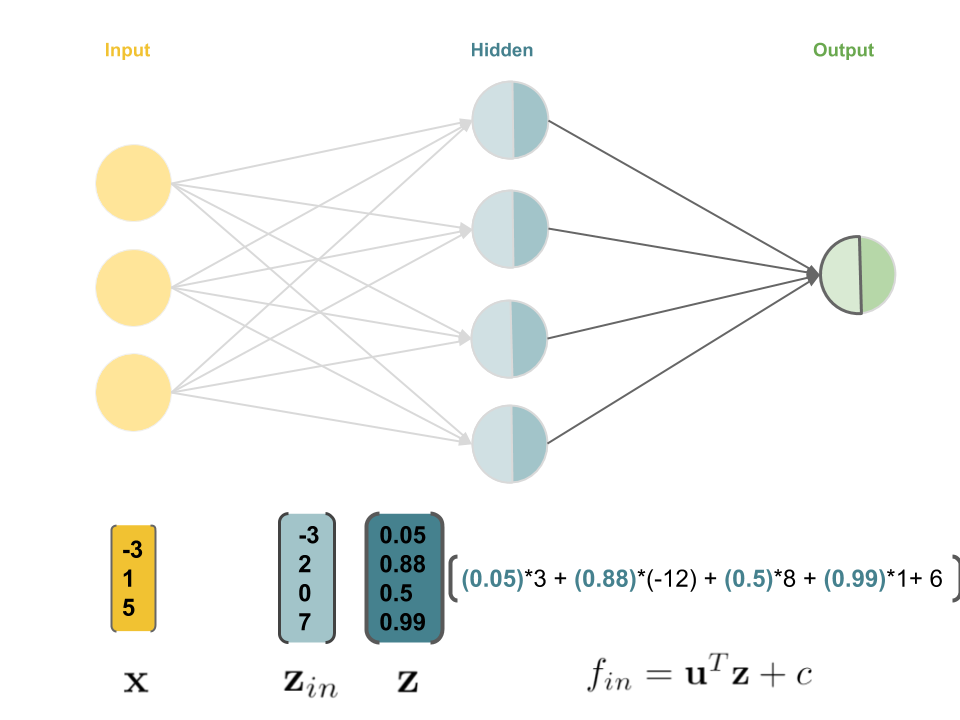
\includegraphics{plots/sinlay_ten.png}}}
    \only<5>{\scalebox{1}{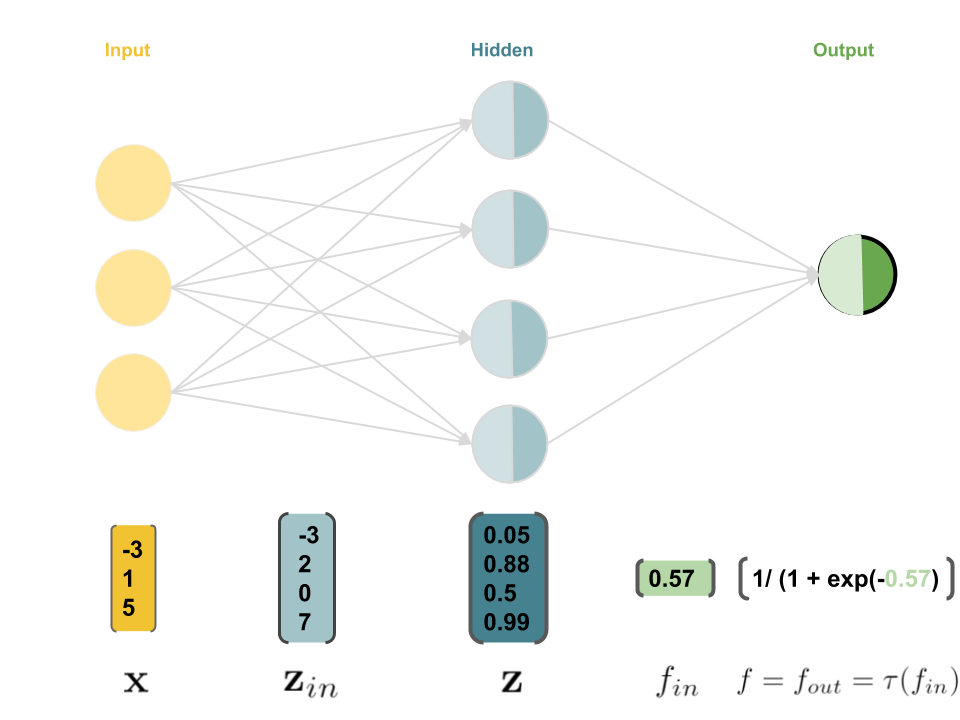
\includegraphics{plots/sinlay_eleven.png}}}
    \only<6>{\scalebox{1}{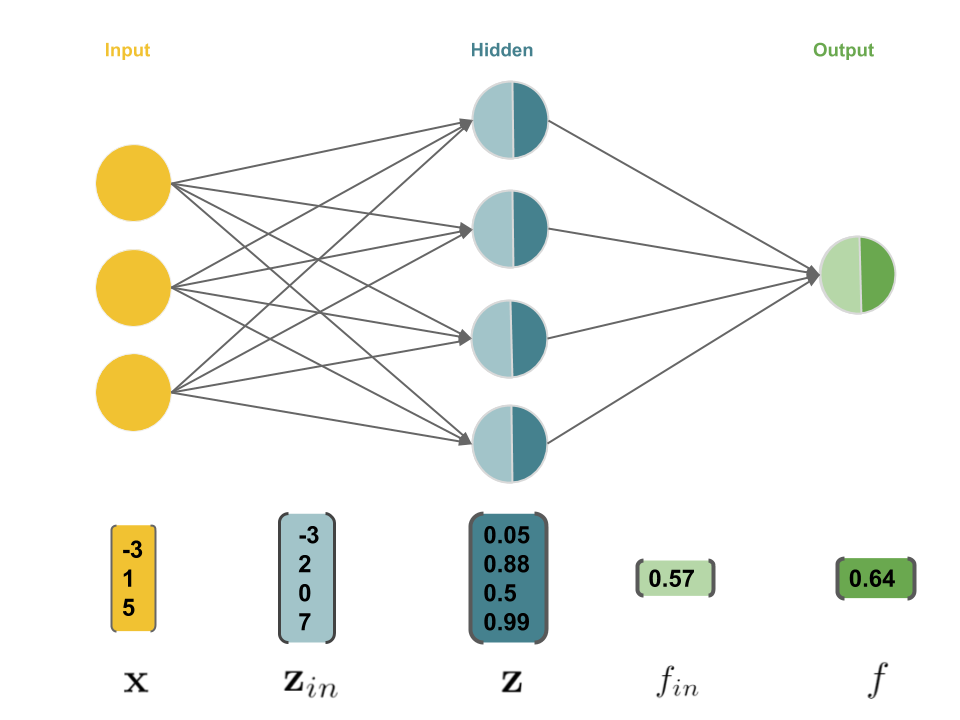
\includegraphics{plots/sinlay_twelve.png}}}
  \end{figure}
\end{frame}

\begin{frame} {Hidden Layer: Activation Function}
  \begin{itemize}
    \item It is important to note that if the hidden layer does not have a non-linear activation, the network can only learn linear decision boundaries.
    % \item To drop the bias term in the notation, let us add a constant feature to $\xv$ which always takes the value
    % $1$, i.e.
    % $$
    % \tilde{\xv} = (1,x_1, \ldots, x_p)^\top
    % $$
    \item For simplification purposes, we drop the bias terms in notation and let $\sigma = \text{id}$. Then:
    \begin{eqnarray*}
        f(\xv) & = & \tau(\wtu^\top \hidz) = \tau(\wtu^\top \sigma(\Wmat^\top \xv)) \\
         & = & \tau(\wtu^\top \sigma(\Wmat^\top \xv)) \\
         & = & \tau(\wtu^\top\Wmat^\top \xv) = \tau(\mathbf{v}^\top \xv)
      \end{eqnarray*}
      where $ \mathbf{v} = \Wmat\wtu$. It can be seen that $f(\xv)$ can only yield a linear decision boundary.
  \end{itemize}
\end{frame}

\begin{frame} {Hidden Layer: Activation Function}
  \begin{blocki}{ReLU activation:}
    \item Currently the most popular choice is the ReLU (rectified linear unit):
    $$ \sigma (v) = \max(0,v) $$
  \end{blocki}
  
\begin{center}
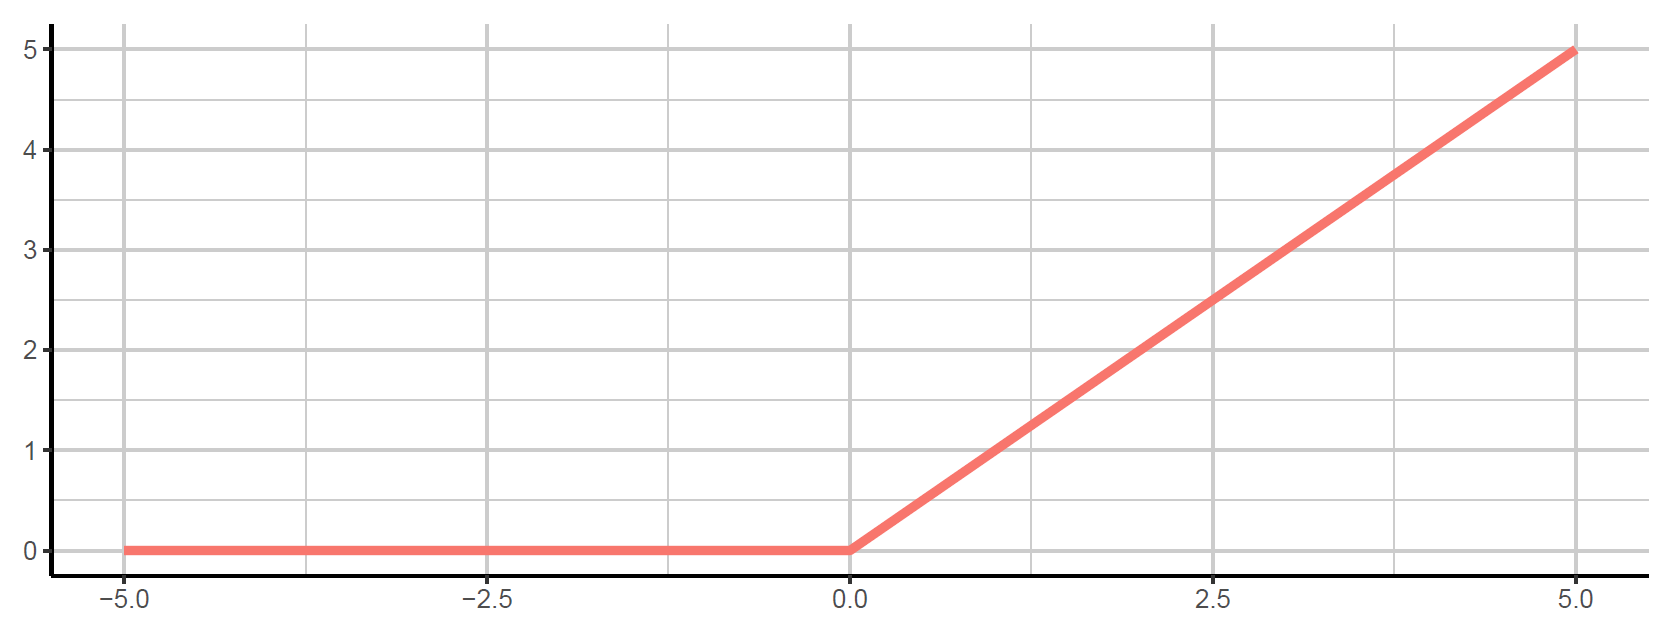
\includegraphics[width=1\textwidth]{plots/ReLU.png}
\end{center}

\end{frame}

\begin{frame} {Hidden Layer: Activation Function}
  \begin{itemize}
    \item Some important properties of the ReLU function include:
    \item[]
    \item[]
    \begin{itemize}
      \item limits: $$\lim_{v \to -\infty} \sigma(v) = 0 \text{ and } \lim_{v \to \infty} \sigma(v) = \infty$$
      \item derivative: 
      $$\frac{\delta\sigma(v)}{\delta v} =
        \begin{cases}
                                       1 & \text{if $v > 0$} \\
                                       0 & \text{else}
        \end{cases}
      $$
    \end{itemize}
  \end{itemize}
\end{frame}

\begin{frame} {Hidden Layer: Activation Function}
  \begin{blocki}{Hyperbolic tangent activation:}
    \item Another choice might be the hyperbolic tangent function:
    $$ \sigma (v) = \text{tanh}(v) = \frac{\text{sinh}(v)}{\text{cosh}(v)} = 1 - \frac{2}{\exp(2v) + 1}$$
  \end{blocki}
  
\begin{center}
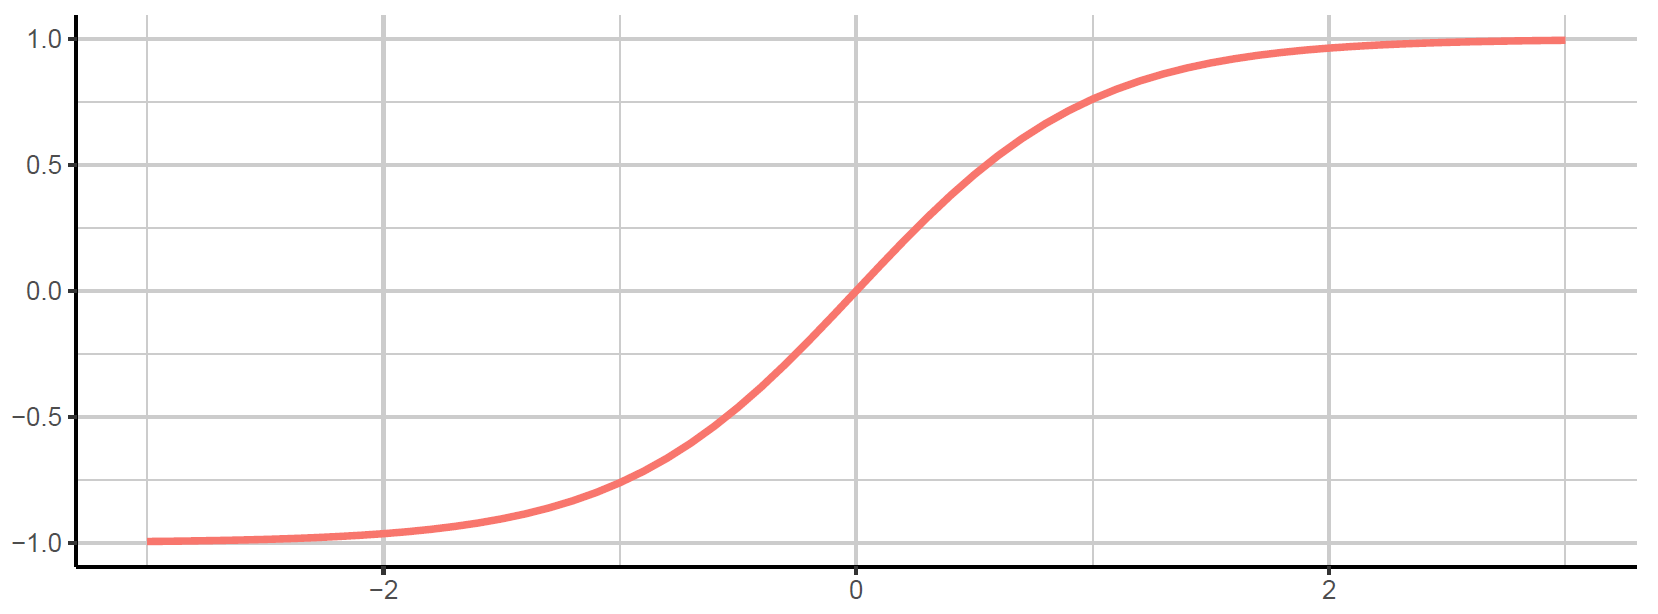
\includegraphics[width=1\textwidth]{plots/tanh.png}
\end{center}

\end{frame}

\begin{frame} {Hidden Layer: Activation Function}
  \begin{itemize}
    \item Some important properties of the hyperbolic tangent function include:
    \item[]
    \item[]
    \begin{itemize}
      \item limits: $$\lim_{v \to -\infty} \sigma(v) = -1 \text{ and } \lim_{v \to \infty} \sigma(v) = 1$$
      \item derivative: $$\frac{\delta\sigma(v)}{\delta v} = 1 - \text{tanh}^2(v)$$
      \item symmetry: $$\sigma(v) \text{ is rotationally symmetric about } (0, 0)$$ \\
      % https://en.wikipedia.org/wiki/Even_and_odd_functions
      (that is, a rotation of $180^{\circ}$ does not change the graph of the function.)
    \end{itemize}
  \end{itemize}
\end{frame}

\begin{frame} {Hidden Layer: Activation Function}
  \begin{blocki}{Sigmoid activation function:}
  \item Of course, as seen in the previous example, the sigmoid function can be used even in the hidden layer:
    $$ \sigma(v) = \frac{1}{1+\exp (-v)} $$
  \end{blocki}
  
\begin{center}
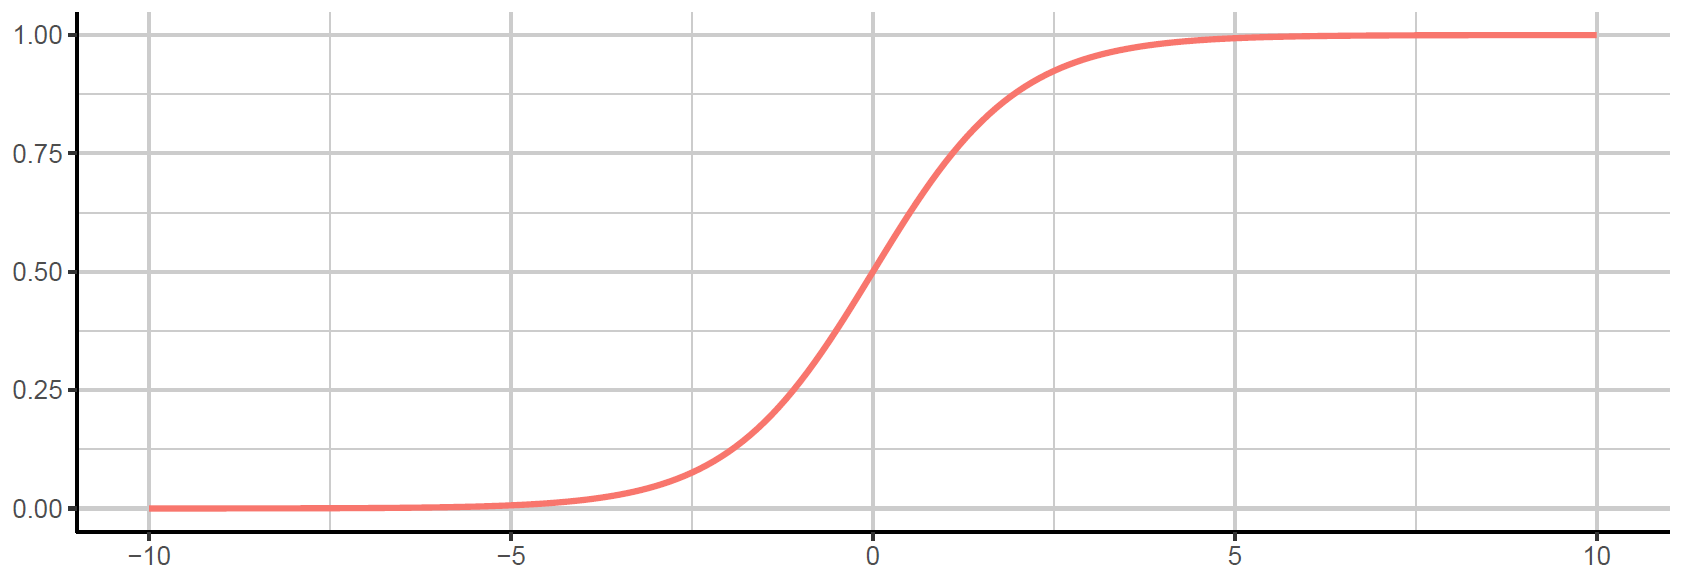
\includegraphics[width=1\textwidth]{plots/Sigmoid.png}
\end{center}

\end{frame}
\begin{frame}{Hidden Layer: Activation Function}
  \begin{itemize}
    \item Some important properties of the logistic sigmoid function include:
    \item[]
    \item[]
    \begin{itemize}
      \item limits: $$\lim_{v \to -\infty} \sigma(v) = 0 \text{ and } \lim_{v \to \infty} \sigma(v) = 1$$
      \item the derivative: $$\frac{\delta\sigma(v)}{\delta v}=\frac{\exp(v)}{(1+\exp(v))^2} = \sigma(v)(1-\sigma(v))$$
      \item symmetry: $$\sigma(v) \text{ is rotationally symmetric about } (0, 0.5)$$ 
            
    \end{itemize}
  \end{itemize}
\end{frame}
%%%%%%%%%%%%%%%%%%%%%%%%%%%%%%%%%%%%%%%%%%%%%%%%%%%%%%%%%%%%%%%%%%
\begin{vbframe}{Example: XOR Problem}
  \begin{itemize}
    \item Suppose we have four data points $$X = \{(0,0)^\top, (0,1)^\top, (1,0)^\top, (1,1)^\top \}$$
    \item The XOR gate (exclusive or) returns true, when an odd number of inputs are true:
  \end{itemize}
  \begin{table}
    \centering
      \begin{tabular}{ccc}
        \textbf{$x_1$}  & \textbf{$x_2$}  & \textbf{XOR} $= y$ \\
        \hline
        \hline
        $0$             &   $0$           &  $0$ \\
        $0$             &   $1$           &  $1$ \\
        $1$             &   $0$           &  $1$ \\
        $1$             &   $1$           &  $0$
      \end{tabular}
  \end{table}
  \begin{itemize}
    \item Can you learn the target function with a logistic regression model? \\
    % (Aside from statistical generalization, we just want to learn the training data!)
  \end{itemize}
\framebreak
  \begin{minipage}{0.45\textwidth}
    \begin{itemize}
      \item Logistic regression can not solve this problem. %and will always output $0.5$. \\
      In fact, any model using simple hyperplanes for separation can not (including a single neuron).
      \lz
      \item A small neural net can easily solve the problem by transforming the space!
    \end{itemize}
  \end{minipage}
  \begin{minipage}{0.5\textwidth}
    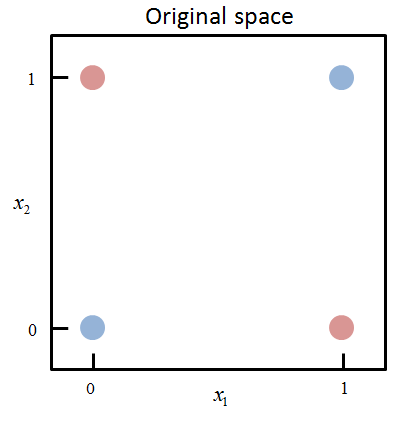
\includegraphics{plots/xor1.png}%
  \end{minipage}\hfill
\framebreak
  \begin{itemize}
    \item Consider the following model:
  \end{itemize}
    \begin{figure}
      \centering
        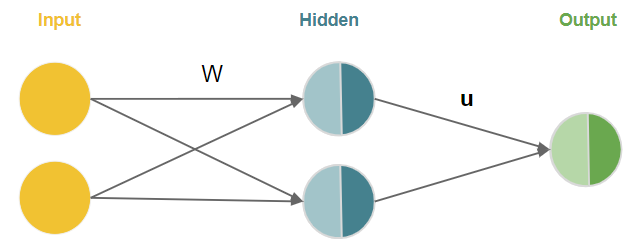
\includegraphics[width=8cm]{plots/xor_rep.png}%
        \caption{A neural network with two neurons in the hidden layer. The matrix $\Wmat$ describes the mapping from $\xv$ to $\hidz$. The vector $\wtu$ from $\hidz$ to $y$.}
    \end{figure}
\framebreak
  \begin{itemize}
    \item Let use ReLU $\sigma(z) = \max\left\{0, z \right\}$ as activation function and a simple thresholding function $\tau(z) = [ z > 0 ] =  \begin{cases} 1 & \text{ if } z > 0 \\ 0 & \text{otherwise} \end{cases} $ \\ as output transformation function. We can represent the architecture of the model by the following equation: 
  \end{itemize}
  \begin{eqnarray*}
    f(\xv~|~\thetab) &=& f(\xv~|~ \Wmat, \biasb, \wtu, \biasc) = \tau\left(\wtu^\top\sigma(\Wmat^\top \xv+\biasb)+\biasc\right) \\
                &=& \tau\left(\wtu^\top \max\{0, \Wmat^\top \xv+\biasb\} + \biasc\right)
  \end{eqnarray*}
  % \begin{footnotesize}
  % \textbf{Note:} To simplify calculations, we \enquote{falsely} treat the problem as a regression problem (no final output transformation $\tau$ to map scores to $[0, 1]$). We will see later that transformation to $[0, 1]$ is not necessary in this very special case.
  % \end{footnotesize}
  \begin{itemize}
    \item So how many parameters does our model have?
    \begin{itemize}
      \item In a fully connected neural net, the number of connections between the nodes equals our parameters: $$\underbrace{(2 \times 2)}_{W} + \underbrace{(2 \times 1)}_{\biasb} + \underbrace{(2 \times 1)}_{\wtu} + \underbrace{(1)}_{c} = 9$$
    \end{itemize}
  \end{itemize}
\framebreak
  \begin{eqnarray*}
   \text{Let} \ \Wmat = \begin{pmatrix}
      1 & 1 \\
      1 & 1
    \end{pmatrix}, \
      \biasb = \begin{pmatrix}
      0 \\
      -1
    \end{pmatrix}, \
      \wtu = \begin{pmatrix}
      1 \\
      -2
    \end{pmatrix}, \
      c = - 0.5
  \end{eqnarray*}
  \begin{eqnarray*}
    \Xmat = \begin{pmatrix}
      0 & 0 \\
      0 & 1 \\
      1 & 0 \\
      1 & 1
    \end{pmatrix}, \
    \Xmat \Wmat = \begin{pmatrix}
      0 & 0 \\
      1 & 1 \\
      1 & 1 \\
      2 & 2
    \end{pmatrix}, \
      \Xmat \Wmat + \bm{B} = \begin{pmatrix}
        0 & -1 \\
        1 & 0 \\
        1 & 0 \\
        2 & 1
    \end{pmatrix}
  \end{eqnarray*}
%\vspace{4mm}
 \footnotesize{Note: $\Xmat$ is a $(n \times p)$ design matrix in which the \textit{rows} correspond to the data points. $\Wmat$, as usual, is a $(p \times m)$ matrix where each \textit{column} corresponds to a single (hidden) neuron. $\bm{B}$ is a ($n \times m$) matrix with $\biasb$ duplicated along the rows.}
 \begin{figure}
    \centering
      \scalebox{0.6}{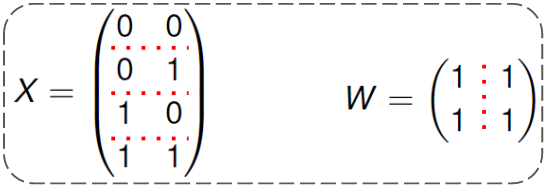
\includegraphics{plots/rowcol.png}}
  \end{figure}
 \framebreak
 \normalsize{
 \begin{eqnarray*}
   \text{Let} \ \Wmat = \begin{pmatrix}
      1 & 1 \\
      1 & 1
    \end{pmatrix}, \
      \biasb = \begin{pmatrix}
      0 \\
      -1
    \end{pmatrix}, \
      \wtu = \begin{pmatrix}
      1 \\
      -2
    \end{pmatrix}, \
      c = - 0.5
  \end{eqnarray*}
  \begin{eqnarray*}
  \Xmat = \begin{pmatrix}
      0 & 0 \\
      0 & 1 \\
      1 & 0 \\
      1 & 1
    \end{pmatrix}, \
    \Xmat\Wmat = \begin{pmatrix}
      0 & 0 \\
      1 & 1 \\
      1 & 1 \\
      2 & 2
    \end{pmatrix}, \
      \Xmat \Wmat + \bm{B} = \begin{pmatrix}
        0 & -1 \\
        1 & 0 \\
        1 & 0 \\
        2 & 1
    \end{pmatrix}
  \end{eqnarray*}
  \begin{eqnarray*}
    \bm{Z} = \max\{0, \Xmat \Wmat+\bm{B}\}
    &=&
    \begin{pmatrix}
      0 & 0 \\
      1 & 0 \\
      1 & 0 \\
      2 & 1
    \end{pmatrix}
  \end{eqnarray*}
  \begin{itemize}
    \item Note that we computed all examples at once.
  \end{itemize}

\framebreak
  \begin{minipage}{0.45\textwidth}
    \begin{itemize}
      \item The input points are mapped into transformed space to
        \begin{eqnarray*}
          \bm{Z} = \begin{pmatrix}
              0 & 0 \\
              1 & 0 \\
              1 & 0 \\
              2 & 1
          \end{pmatrix}
        \end{eqnarray*}
    %  \item[] which is easily separable.
    \end{itemize}
  \end{minipage}
  \begin{minipage}{0.5\textwidth}
    \includegraphics<1>{plots/xor2_2.png}%
  \end{minipage}\hfill
  
\framebreak
  \begin{minipage}{0.45\textwidth}
    \begin{itemize}
      \item The input points are mapped into transformed space to
        \begin{eqnarray*}
          \bm{Z} = \begin{pmatrix}
              0 & 0 \\
              1 & 0 \\
              1 & 0 \\
              2 & 1
          \end{pmatrix}
        \end{eqnarray*}
      \item[] which is easily separable.
    \end{itemize}
  \end{minipage}
  \begin{minipage}{0.5\textwidth}
    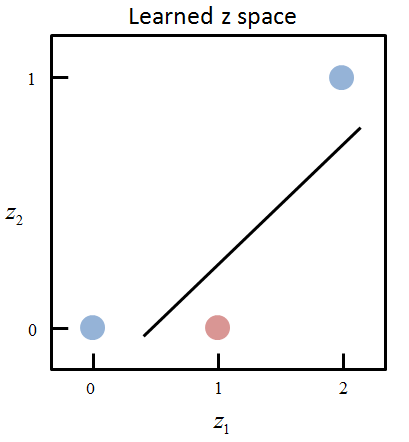
\includegraphics{plots/xor2.png}%
  \end{minipage}\hfill
  
\framebreak
  \begin{itemize}
    \item In a final step we have to multiply the activated values of matrix $\bm{Z}$ with the vector $\wtu$ and add the bias term $c$:
  \end{itemize}
  \begin{eqnarray*}
    f(\xv ~|~ \Wmat, \biasb, \wtu, c) &=&
    \begin{pmatrix}
      0 & 0 \\
      1 & 0 \\
      1 & 0 \\
      2 & 1
    \end{pmatrix}
    \begin{pmatrix}
      1 \\
      -2
    \end{pmatrix} + 
    \begin{pmatrix}
      - 0.5 \\
      - 0.5 \\
      - 0.5 \\
      - 0.5
    \end{pmatrix}
    =
    \begin{pmatrix}
      - 0.5 \\
      0.5 \\
      0.5 \\
      - 0.5
    \end{pmatrix}
  \end{eqnarray*}
  \begin{itemize}
    \item And then apply the step function $\tau(z) = [z > 0 ]$.  This solves the XOR problem perfectly!
  \end{itemize}
  \begin{table}
    \centering
      \begin{tabular}{ccc}
        \textbf{$x_1$}  & \textbf{$x_2$}  & \textbf{XOR} = y\\
        \hline
        \hline
        $0$             &   $0$           &  $0$ \\
        $0$             &   $1$           &  $1$ \\
        $1$             &   $0$           &  $1$ \\
        $1$             &   $1$           &  $0$
      \end{tabular}
  \end{table}
  }
\end{vbframe}

\begin{frame} {Neural Networks: Optimization}
  \begin{itemize}
    \item In this simple example we actually \enquote{guessed} the values of the parameters for $\Wmat$, $\biasb$, $\bm{u}$ and $c$.
    \vspace{3mm}
    \item That will not work for more sophisticated problems!
    \vspace{3mm}
    \item To learn the right weights (and biases), we have to rely on iterative algorithms like gradient descent.
    \vspace{3mm}
    \item An added complication is that the loss function is no longer convex. Therefore, there might not exist a single minimum. 
    \vspace{3mm}
    \item An extremely efficient method to compute gradients called backpropogation will be covered in the next lecture.
  \end{itemize}
\end{frame}
%%%%%%%%%%%%%%%%%%%%%%%%%%%%%%%%%%%%%%%%%%%%%%%%%%%%%%%%%%%%%%%%%%
%%%%%%%%%%%%%%%%%%%%%%%%%%%%%%%%%%%%%%%%%%%%%%%%%%%%%%%%%%%%%%%%%%

\section{Universal Approximation Property}

\begin{vbframe}{Universal Approximation Property}

  \textbf{Theorem.}
  Let $\sigma: \R \to \R$ be a continuous, non-constant, bounded, and
  monotonically increasing function. Let $C \subset \R^p$ be compact,
  and let $\continuous(C)$ denote the space of continuous functions $C \to \R$.
  Then, given a function $g \in \continuous(C)$ and an accuracy $\varepsilon > 0$,
  there exists a hidden layer size $m \in \N$ and a set of coefficients
  $\Wmat_j \in \R^p$, $u_j, b_j \in \R$
  (for $j \in \{1, \dots, m\}$), such that
  $$
    f_m: C \to \R \,;\quad f_m(\xv) = \sum_{j=1}^m u_j \cdot \sigma \Big( \Wmat_j^\top \xv + b_j \Big)
  $$
  is an $\varepsilon$-approximation of $g$, that is,
  $$
    \|f_m - g\|_{\infty}:= \max_{x \in C} |f_m(\xv) - g(\xv)| < \varepsilon
    \enspace.
  $$

  The theorem extends trivially to multiple outputs.

  \framebreak

  \textbf{Corollary.}
  Neural networks with a single sigmoidal hidden layer and linear
  output layer are universal approximators.

  \begin{itemize}
    \item This means that for a given target function $g$ there exists a
    sequence of networks $\big( f_m \big)_{m \in \N}$ that converges
    (pointwise) to the target function.
    \vspace{2mm}
    \item Usually, as the networks come closer and closer to $g$, they
    will need more and more hidden neurons.
    \vspace{2mm}
    \item A network with fixed layer sizes can only model a subspace of all
    continuous functions. Its dimensionality is limited by the number
    of weights.
    \vspace{2mm}
    \item The continuous functions form an infinite dimensional vector space.
    Therefore arbitrarily large hidden layer sizes are needed.
  \end{itemize}

  \framebreak

  \begin{itemize}
  \item Why is universal approximation a desirable property?
  \vspace{2mm}
  \item Recall the definition of a Bayes optimal hypothesis $h^*: \Xspace \to \Yspace$.
    It is the best possible hypothesis (model) for the given problem:
    it has minimal loss averaged over the data generating distribution.
  \vspace{2mm}
  \item So ideally we would like the neural network (or any other
    learner) to approximate the Bayes optimal hypothesis.
  \vspace{2mm}
  \item Usually we do not manage to learn $h^*$.
  \vspace{2mm}
  \item This is because we do not have enough (infinite) data. We have
    no control over this, so we have to live with this limitation.
  \vspace{2mm}
  \item But we do have control over which model class we use.
  \end{itemize}

  \framebreak

  \begin{itemize}
    \vspace{10mm}
    \item Universal approximation $\Rightarrow$ approximation error tends
    to zero as hidden layer size tends to infinity.
    \vspace{5mm}
    \item Positive approximation error implies that no matter how good
    the data, we cannot find the optimal model.
    \vspace{5mm}
    \item This bears the risk of systematic under-fitting, which can be avoided with a universal model class.
  \end{itemize}

  \framebreak

  \begin{itemize}
    \vspace{5mm}
    \item As we know, there are also good reasons for restricting the model class.
    \vspace{5mm}
    \item This is because a flexible model class with universal approximation
    ability often results in over-fitting, which is no better than
    under-fitting.
    \vspace{5mm}
    \item Thus, \enquote{universal approximation $\Rightarrow$ low approximation error}, but at the risk of a substantial generalization error.
    \vspace{5mm}
    \item In general, models of intermediate flexibility give the best predictions.
    For neural networks this amounts to a reasonably sized hidden layer.
  \end{itemize}
\end{vbframe}

\begin{frame}{NNs as (non-)parametric models}

\only<1->{\textbf{Question:} Are NNs parametric or non-parametric models? }
\only<2->{
\begin{itemize}
  \item Parametric models assume some finite set of model parameters. So the complexity of the model is bounded even if the amount of training data is unbounded. This makes them not very flexible. \\
  Example: Linear Model.
 \item A model is non-parametric, if the number of parameters is not fixed. Complexity of the model can grow as the amount of data grows. This makes them very flexible. \\
 Example: k-NN. 
\end{itemize}
}

\only<3>{If the architecture (here: the size of the hidden layer) is fixed, the number of trainable parameters is fixed and NNs are to be seen as parametric models. 

However, if we do not restrict the hidden layer size prior to training but integrate optimizing the hidden layer size into training, NNs can also be seen as non-parametric models. }

\end{frame}



%%%%%%%%%%%%%%%%%%%%%%%%%%%%%%%%%%%%%%%%%%%%%%%%%%%%%%%%%%%%%%%%%%
%%%%%%%%%%%%%%%%%%%%%%%%%%%%%%%%%%%%%%%%%%%%%%%%%%%%%%%%%%%%%%%%%%
%%%%%%%%%%%%%%%%%%%%%%%%%%%%%%%%%%%%%%%%%%%%%%%%%%%%%%%%%%%%%%%%%%
%%%%%%%%%%%%%%%%%%%%%%%%%%%%%%%%%%%%%%%%%%%%%%%%%%%%%%%%%%%%%%%%%%
\begin{frame} {Neural Nets: Regression/Classification}
  \begin{itemize}
    \vspace{15mm}
    \item Let us look at a few examples of the types of functions and decisions boundaries learnt by neural networks (with a \textbf{single} hidden layer) of various sizes.
       \vspace{5mm} 
    \item \enquote{size} here refers to the number of neurons in the hidden layer.
    \vspace{5mm}
    \item The number of  \enquote{iterations} in the following slides is the number of steps of the applied iterative optimization algorithm (stochastic gradient descent).
  \end{itemize}
\end{frame}

% \begin{vbframe}{Regression: 100 training iterations}
% <<echo=FALSE, warning=FALSE, message=FALSE, results="hide">>=
% 
% library("mlr")
% set.seed(1234L)
% n = 50L
% x = sort(10 * runif(n))
% y = sin(x) + 0.2 * rnorm(x)
% df = data.frame(x = x, y = y)
% tsk = makeRegrTask("sine function example", data = df, target = "y")
% plotLearnerPrediction("regr.nnet", tsk, size = 1L, maxit = 100)
% 
% plotLearnerPrediction("regr.nnet", tsk, size = 2L, maxit = 100)
% 
% plotLearnerPrediction("regr.nnet", tsk, size = 3L, maxit = 100)
% 
% plotLearnerPrediction("regr.nnet", tsk, size = 4L, maxit = 100)
% 
% plotLearnerPrediction("regr.nnet", tsk, size = 5L, maxit = 100)
% 
% plotLearnerPrediction("regr.nnet", tsk, size = 6L, maxit = 100)
% 
% plotLearnerPrediction("regr.nnet", tsk, size = 100L, maxit = 100)
% 
% @
% \end{vbframe}
%%%%%%%%%%%%%%%%%%%%%%%%%%%%%%%%%%%%%%%%%%%%%%%%%%%%%%%%%%%%%%%%%%
%%%%%%%%%%%%%%%%%%%%%%%%%%%%%%%%%%%%%%%%%%%%%%%%%%%%%%%%%%%%%%%%%%
\begin{frame}{Regression: 1000 training iterations}

\only<1>{

\begin{center}
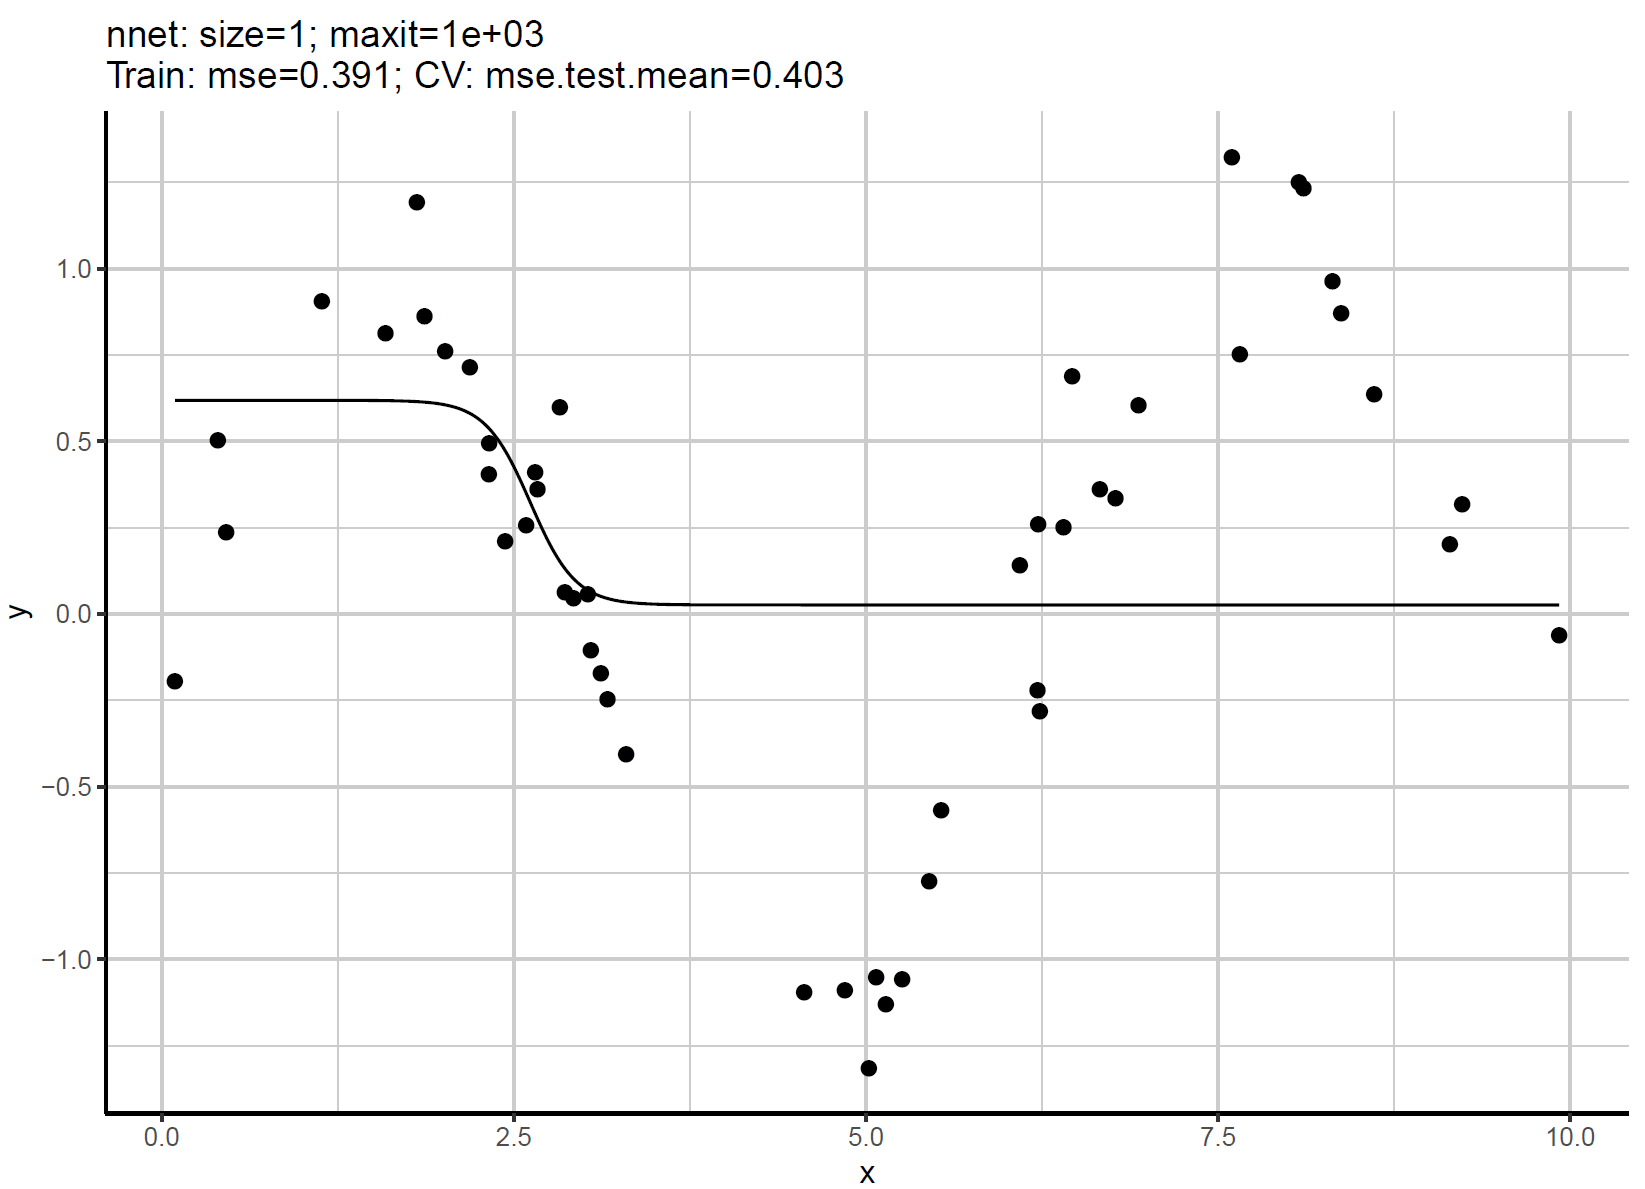
\includegraphics[width=0.9\textwidth]{plots/reg-n1.png}
\end{center}

}

\only<2>{

\begin{center}
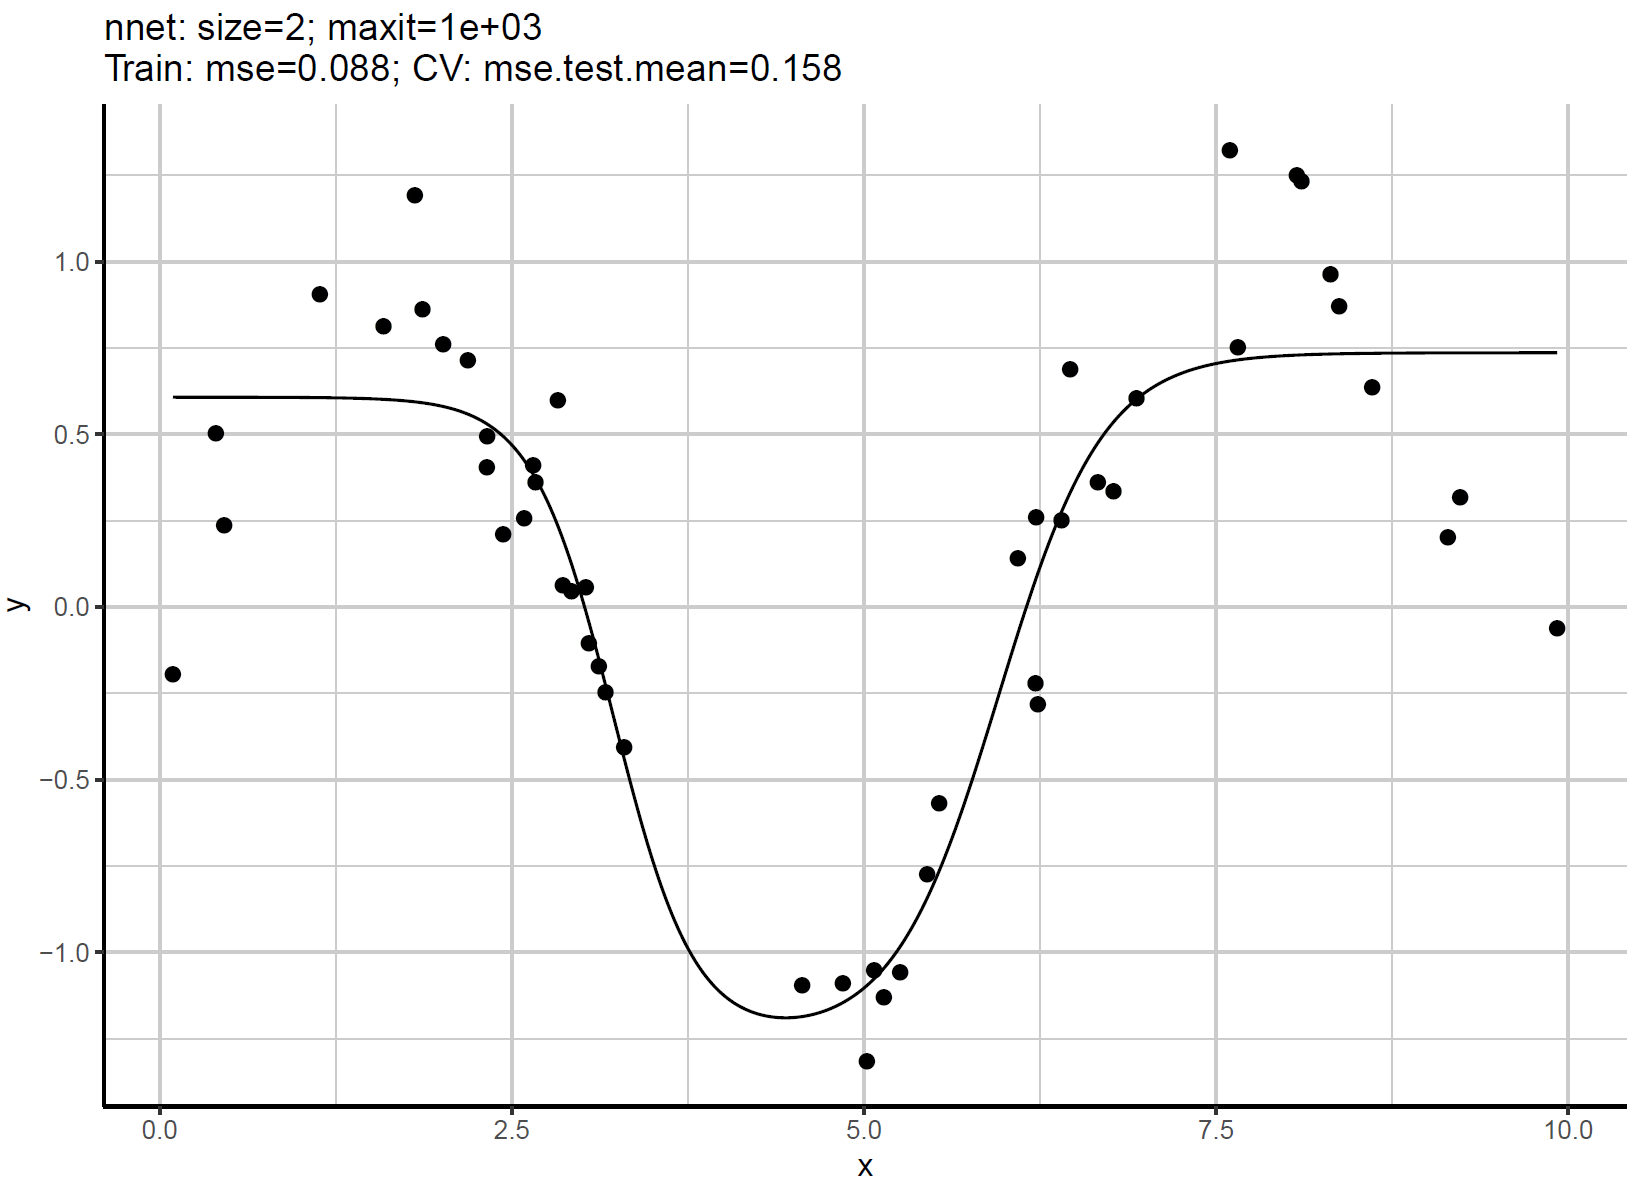
\includegraphics[width=0.9\textwidth]{plots/reg-n2.png}
\end{center}

}

\only<3>{

\begin{center}
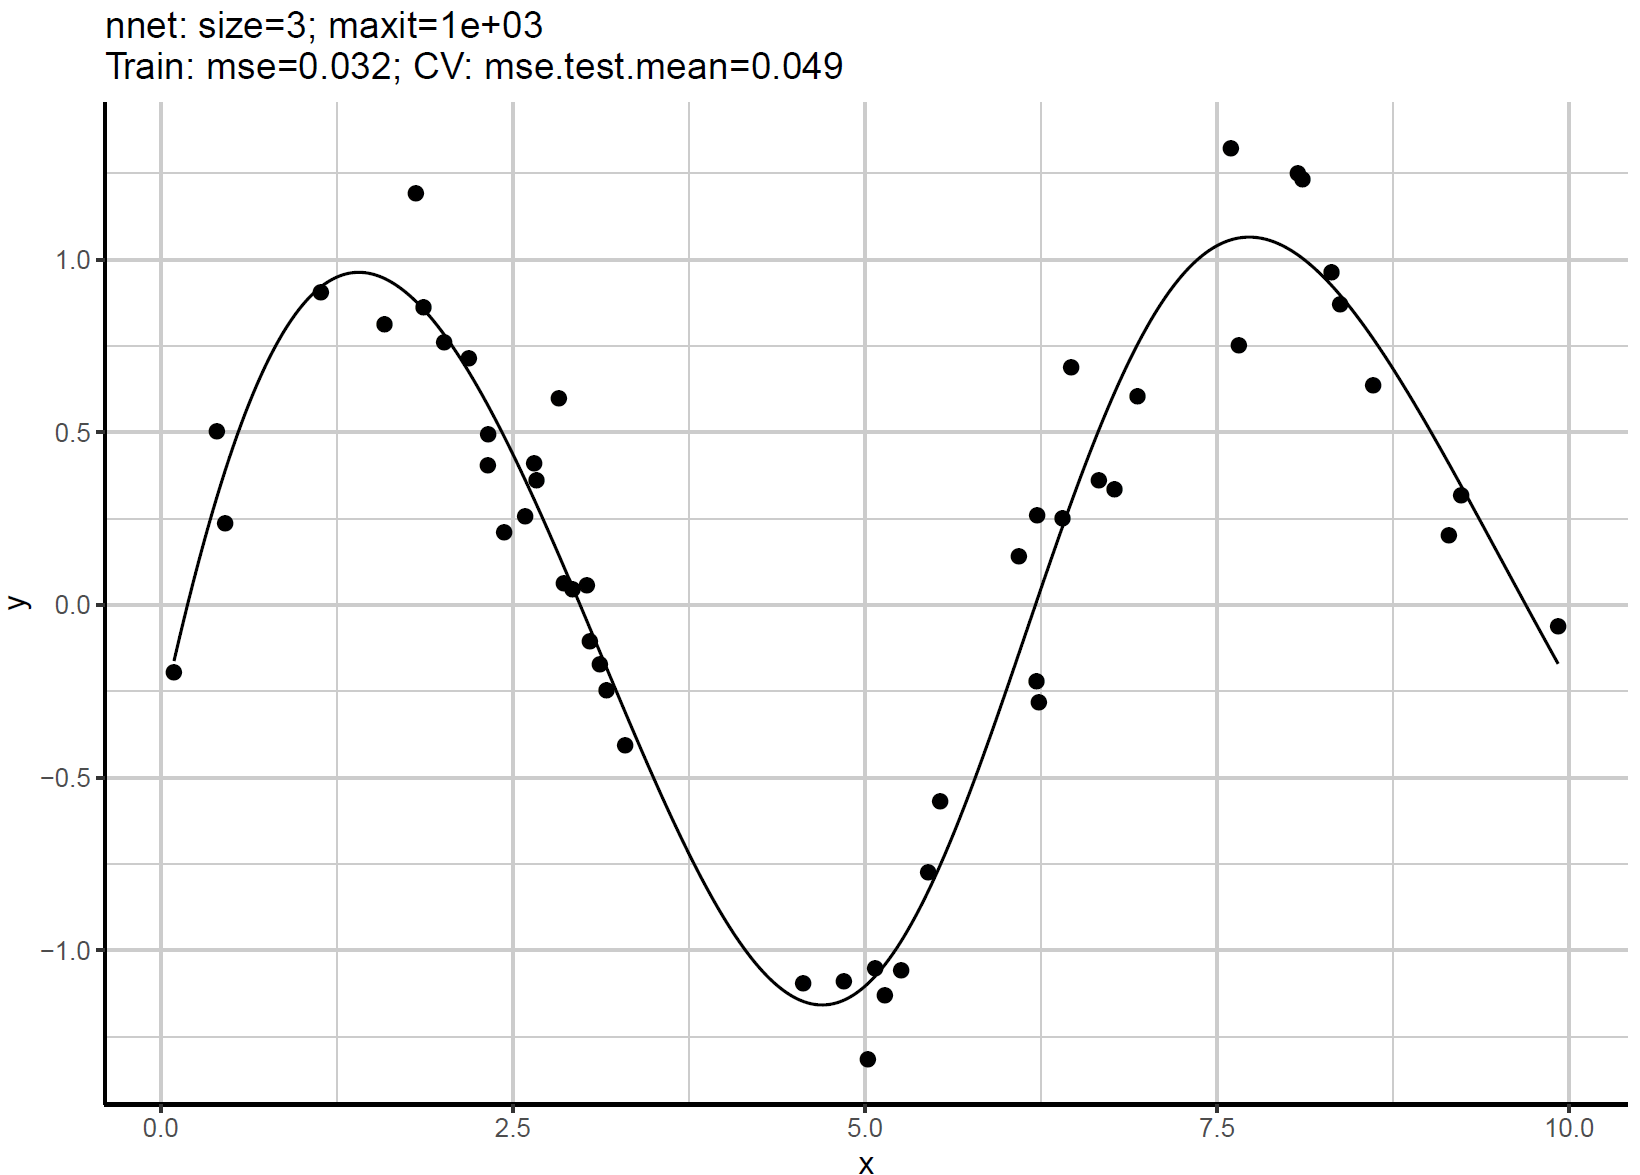
\includegraphics[width=0.9\textwidth]{plots/reg-n3.png}
\end{center}

}

\only<4>{

\begin{center}
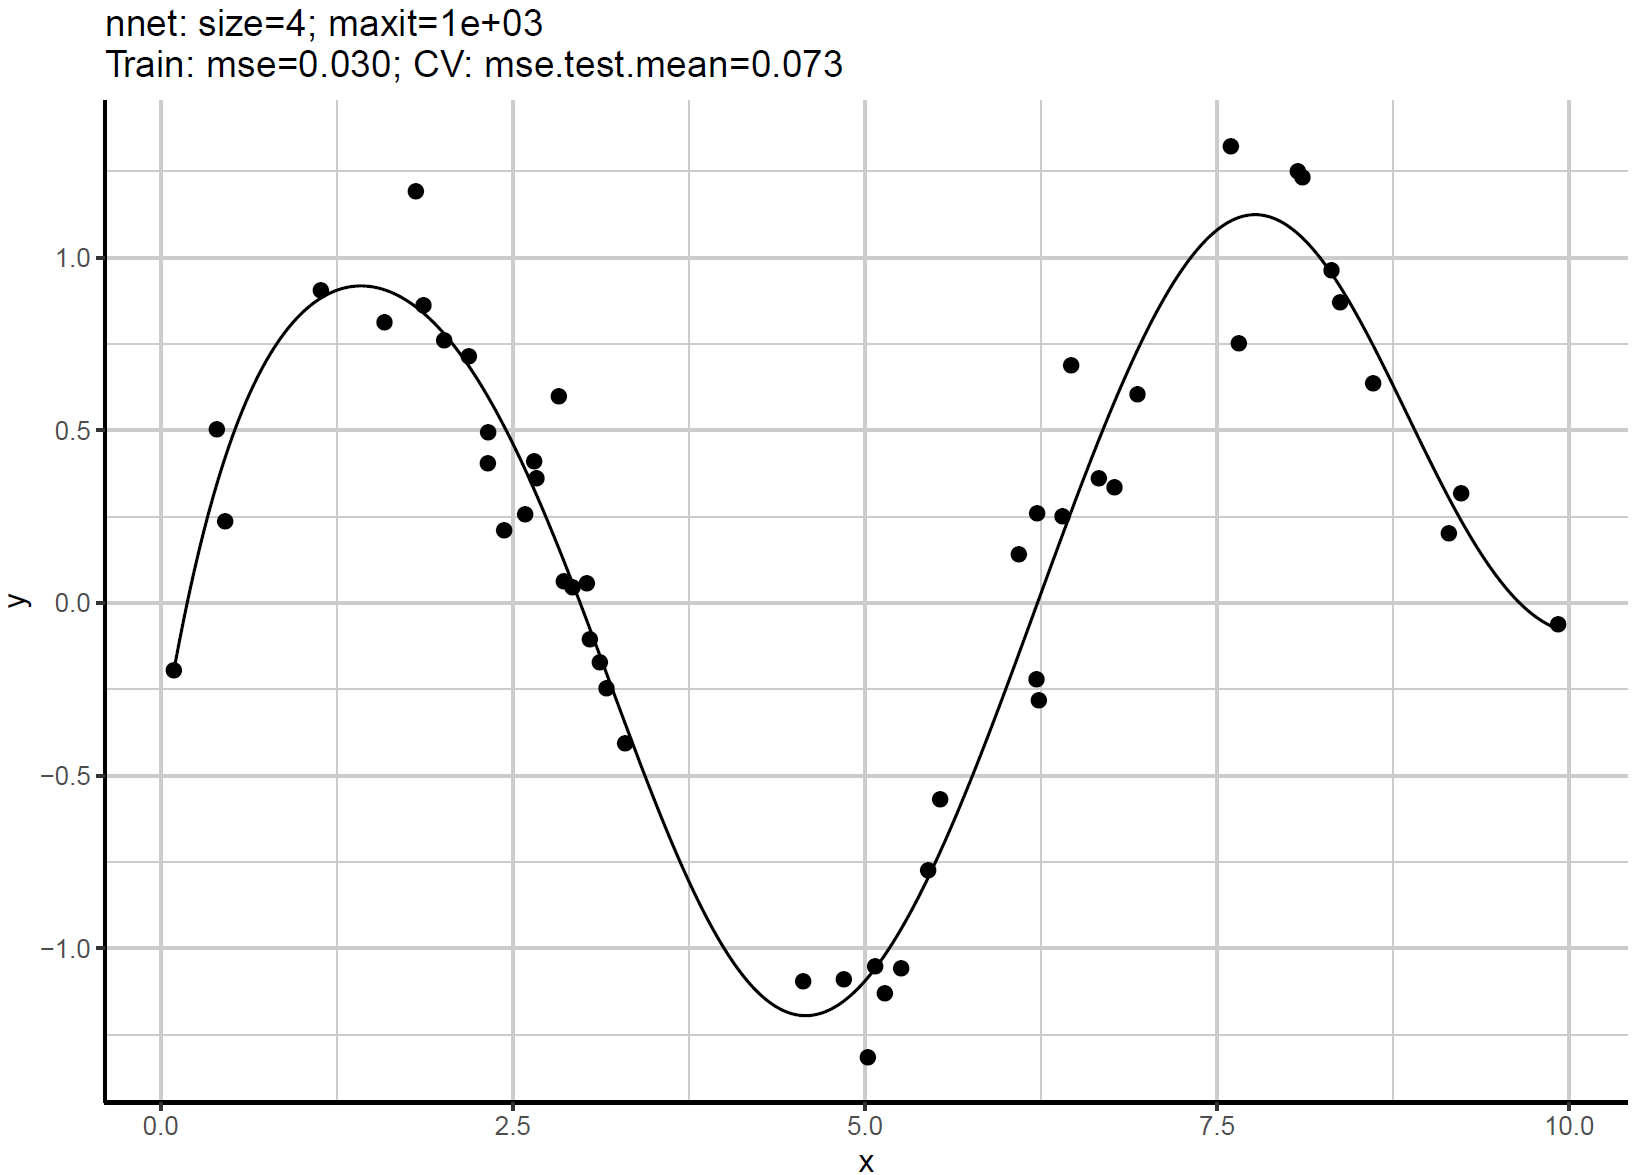
\includegraphics[width=0.9\textwidth]{plots/reg-n4.png}
\end{center}

}

\only<5>{

\begin{center}
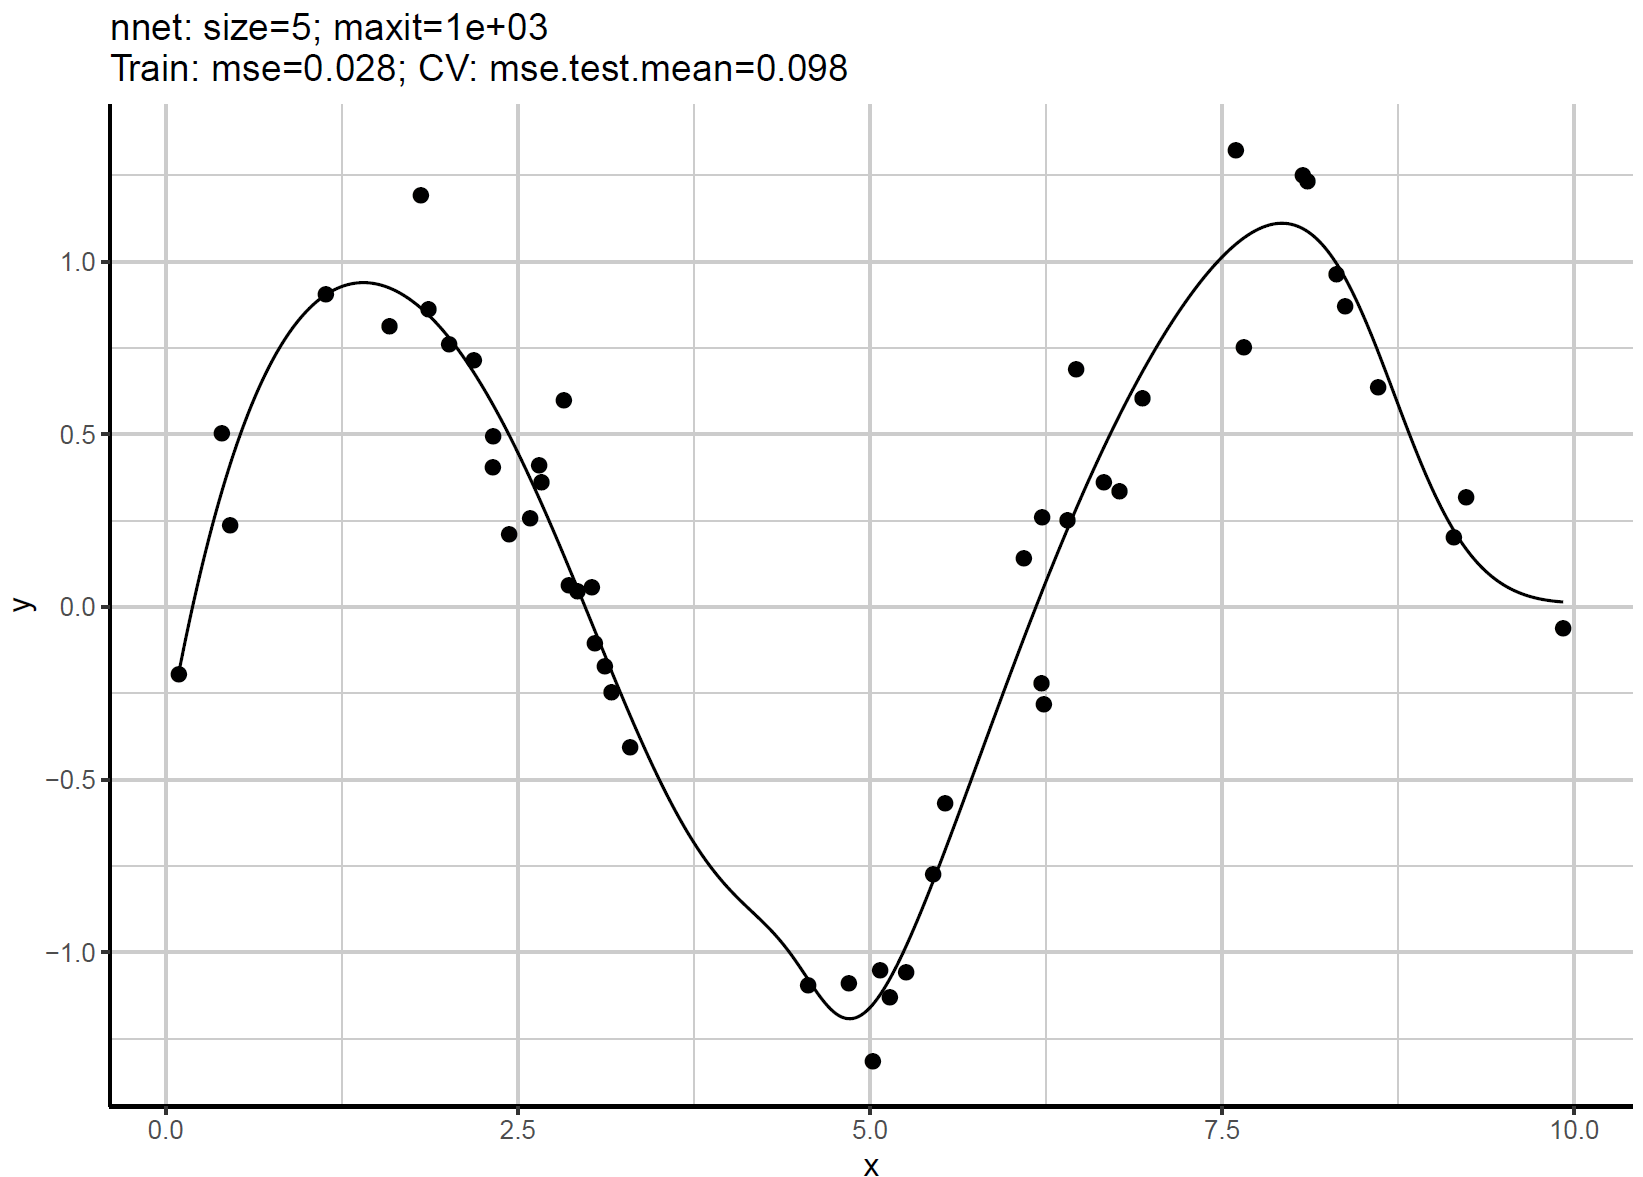
\includegraphics[width=0.9\textwidth]{plots/reg-n5.png}
\end{center}

}

\only<6>{

\begin{center}
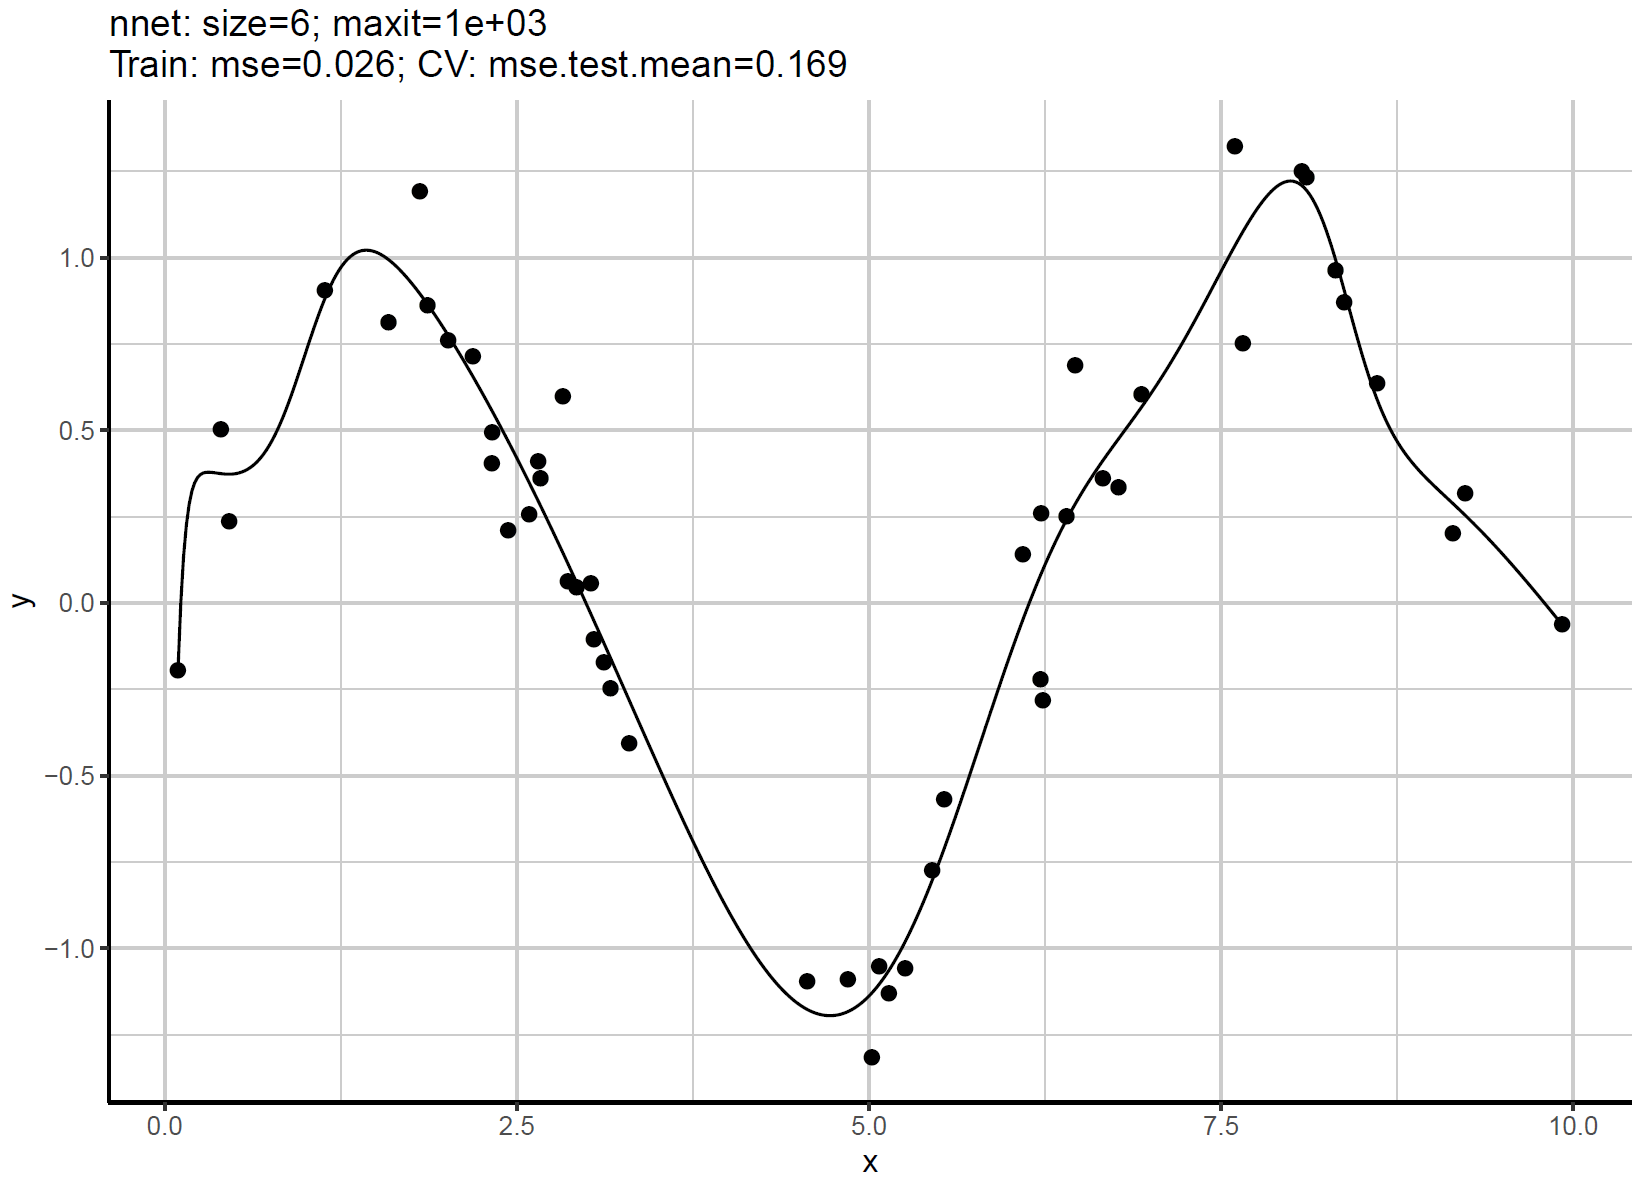
\includegraphics[width=0.9\textwidth]{plots/reg-n6.png}
\end{center}

}

\only<7>{

\begin{center}
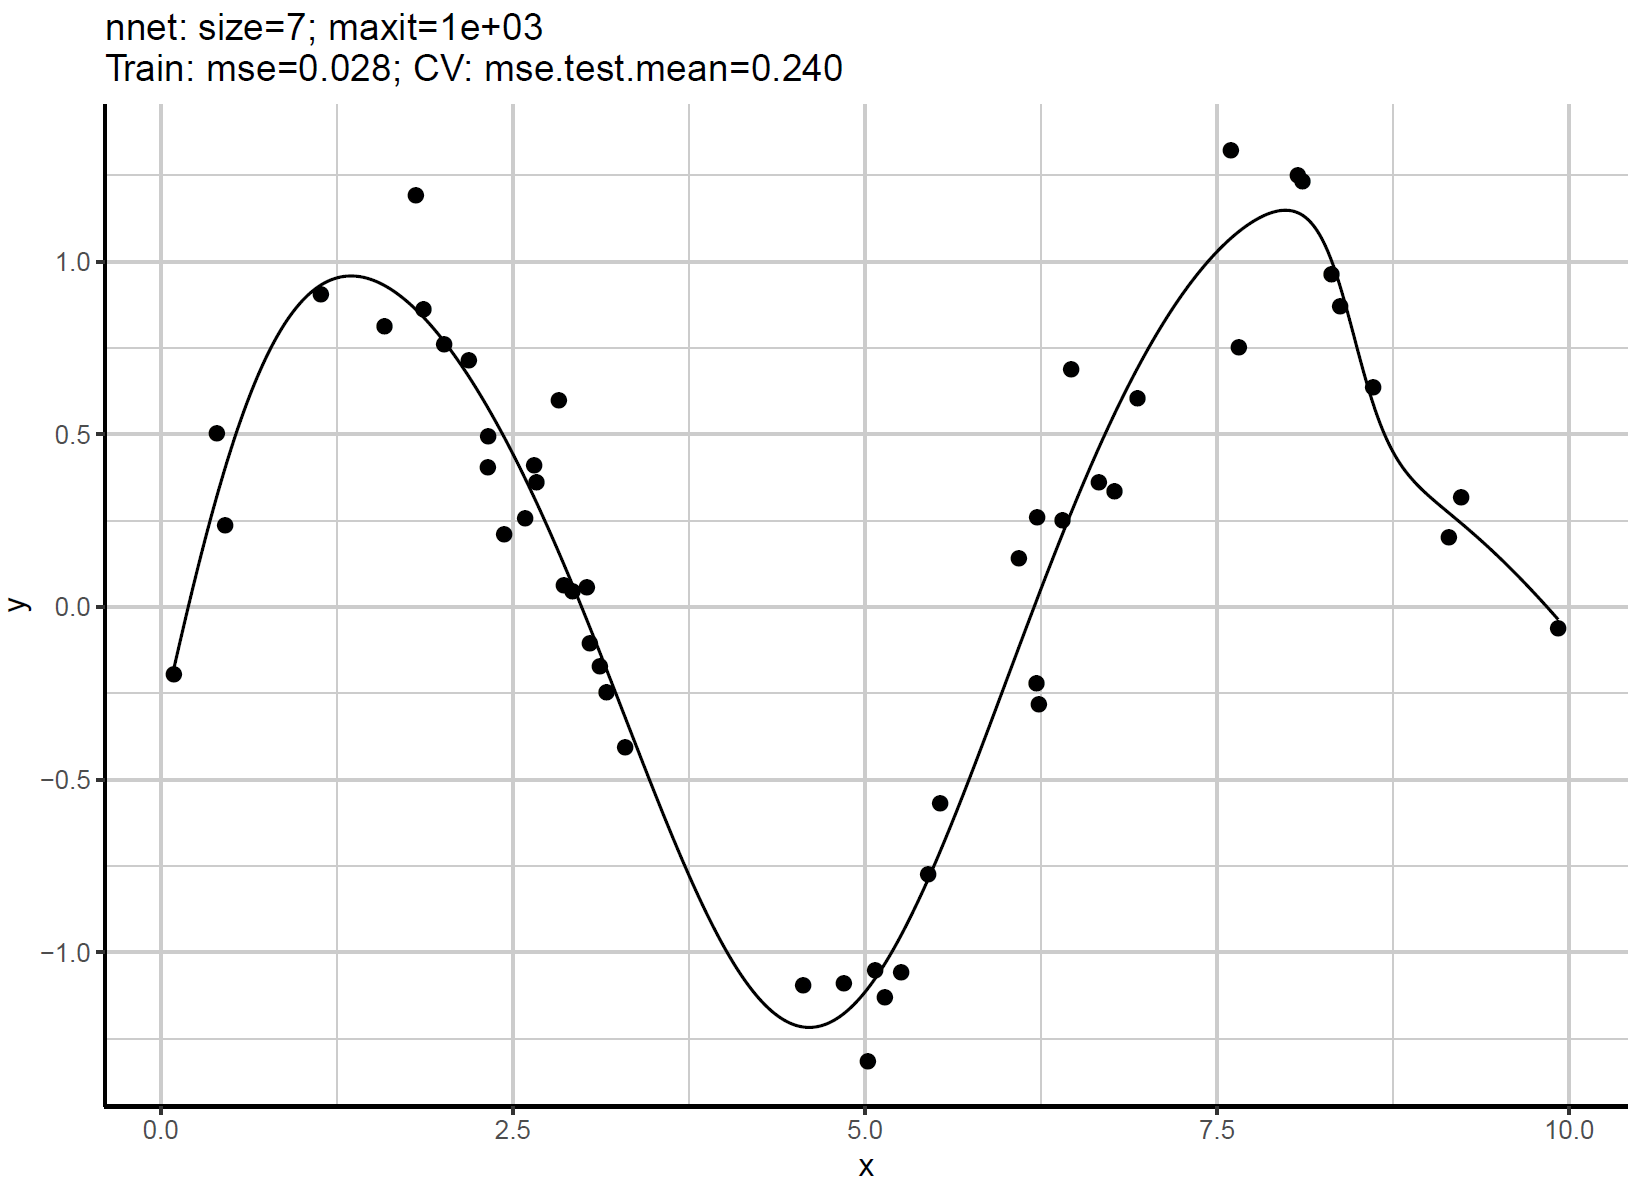
\includegraphics[width=0.9\textwidth]{plots/reg-n7.png}
\end{center}

}

\only<8>{

\begin{center}
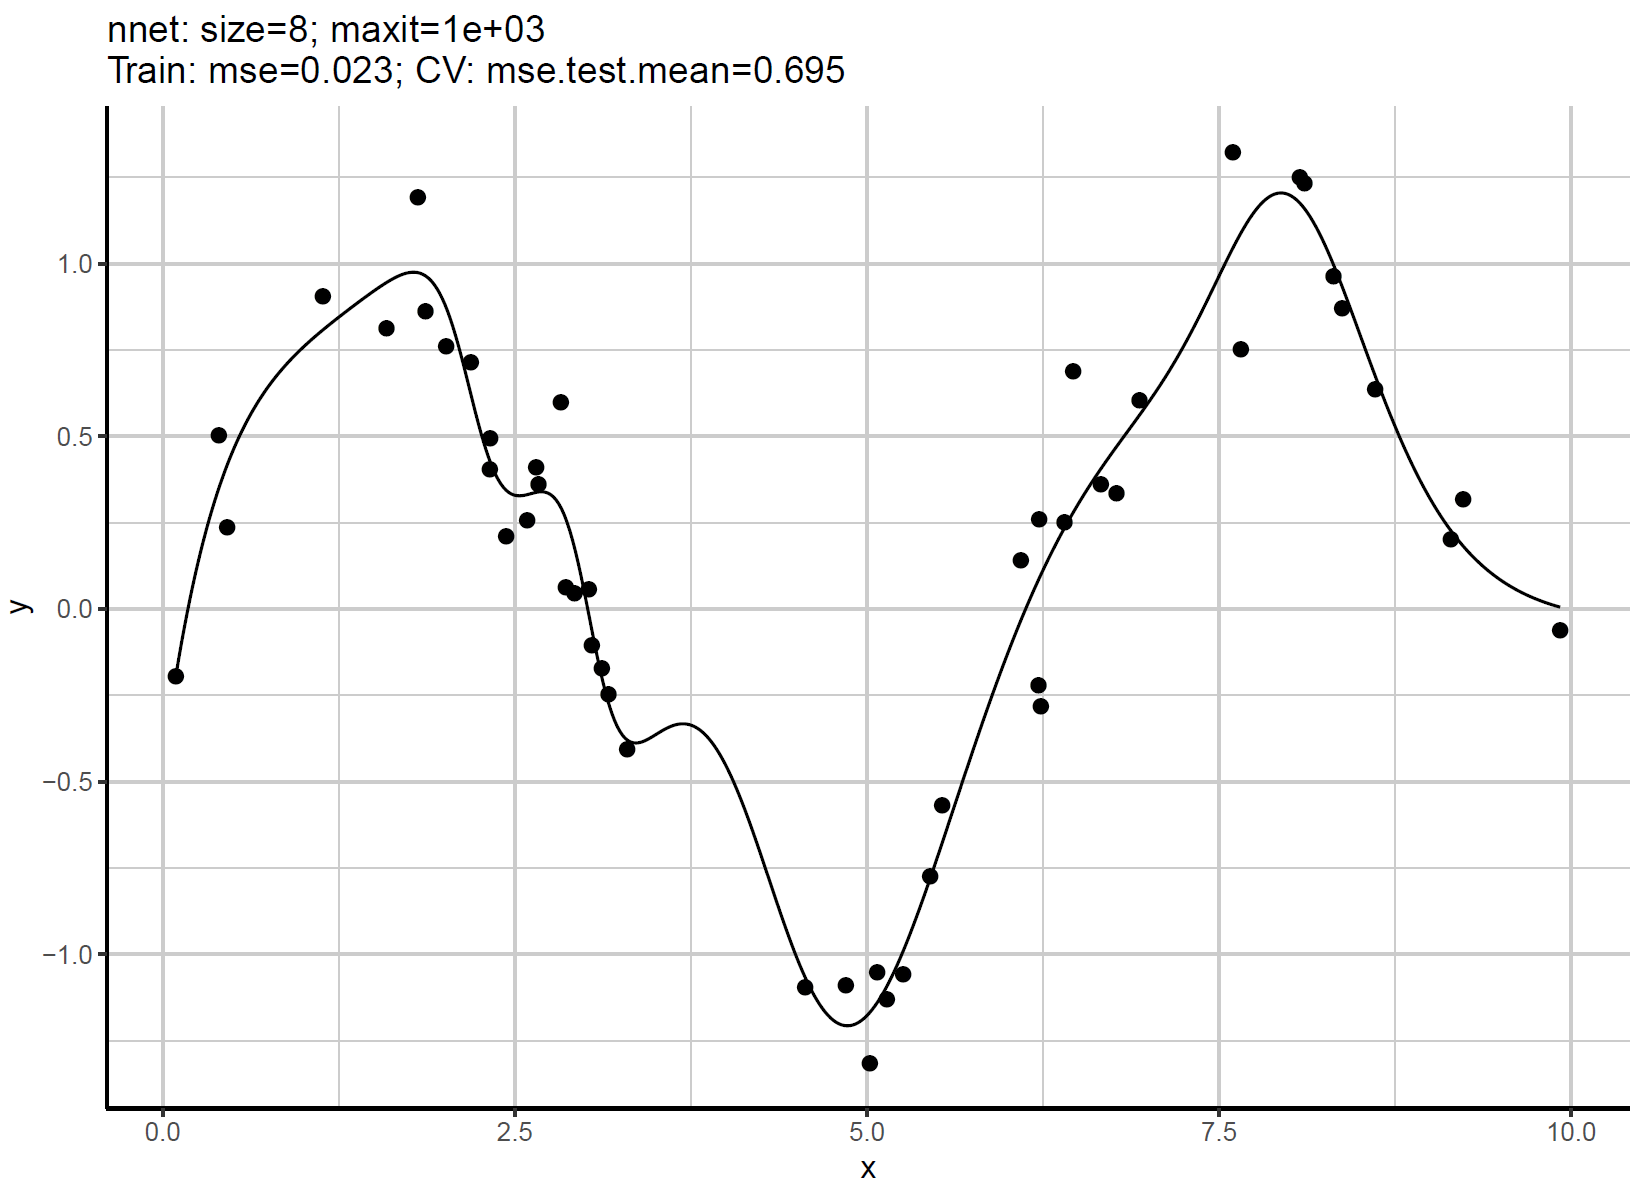
\includegraphics[width=0.9\textwidth]{plots/reg-n8.png}
\end{center}

}

\only<9>{

\begin{center}
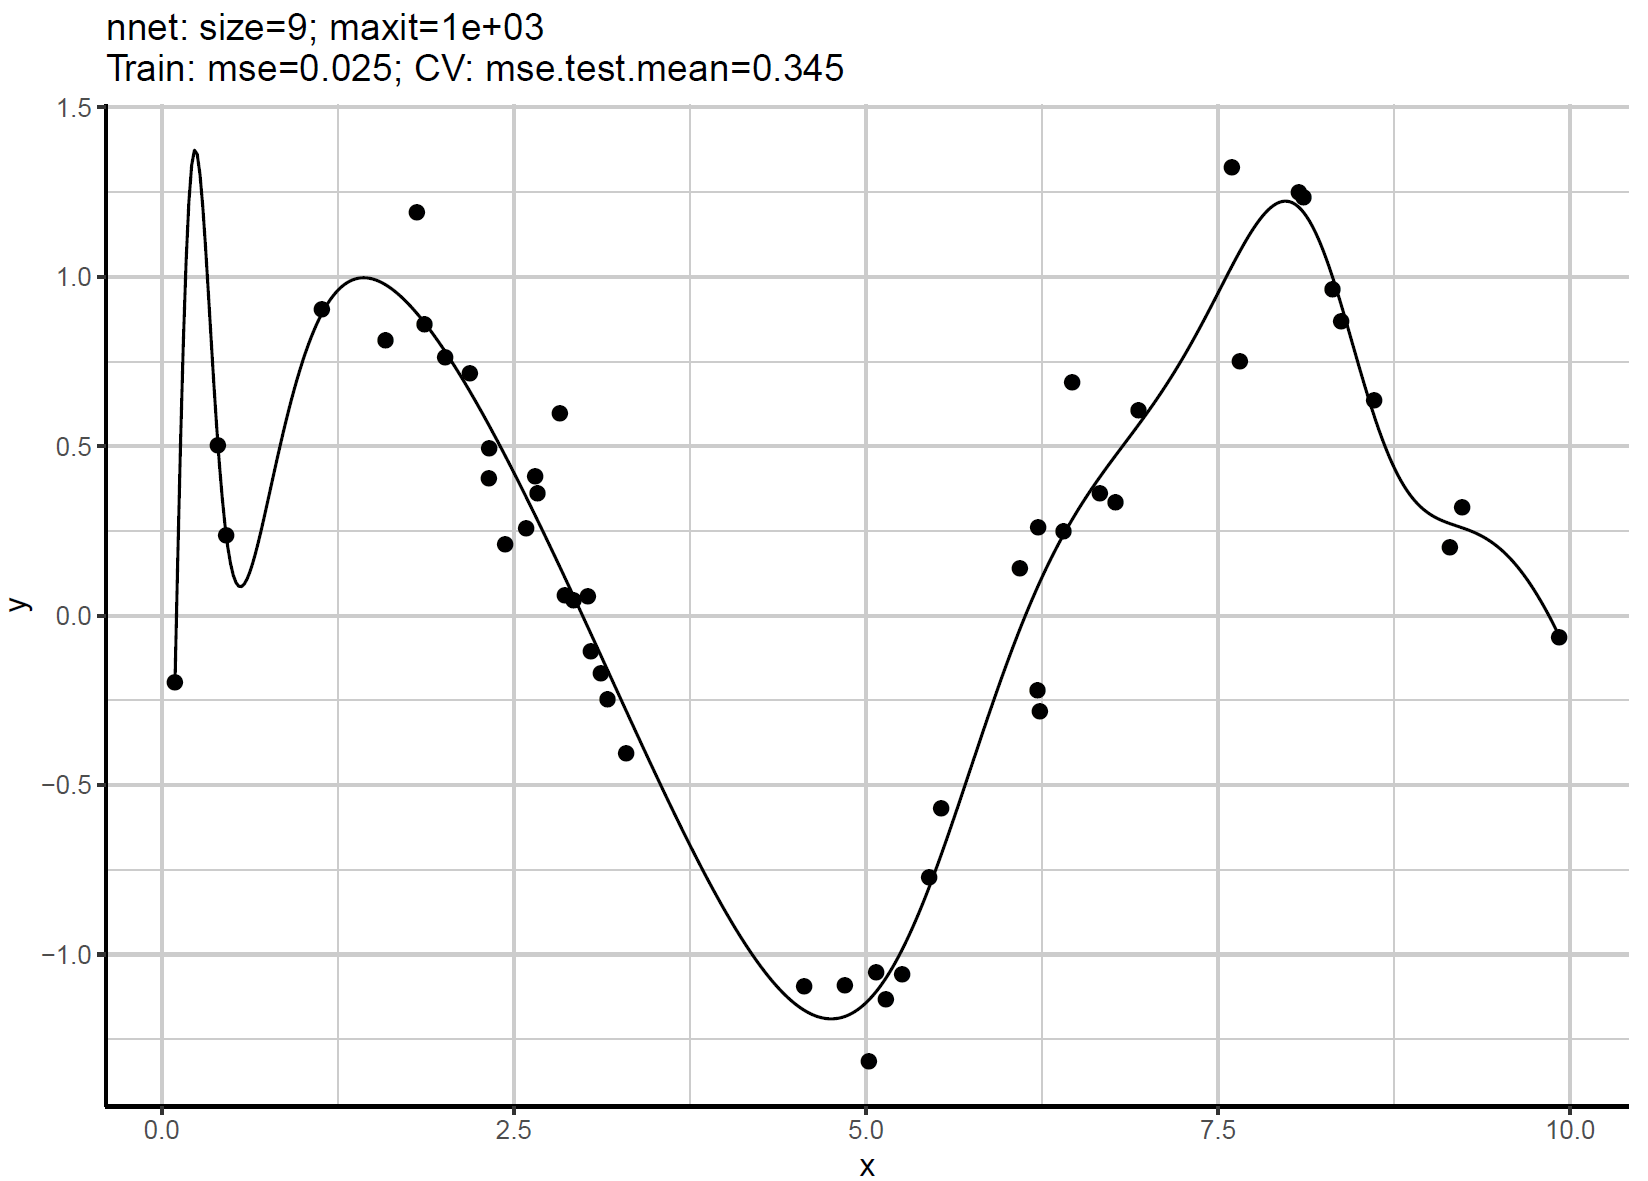
\includegraphics[width=0.9\textwidth]{plots/reg-n9.png}
\end{center}

}

\only<10>{

\begin{center}
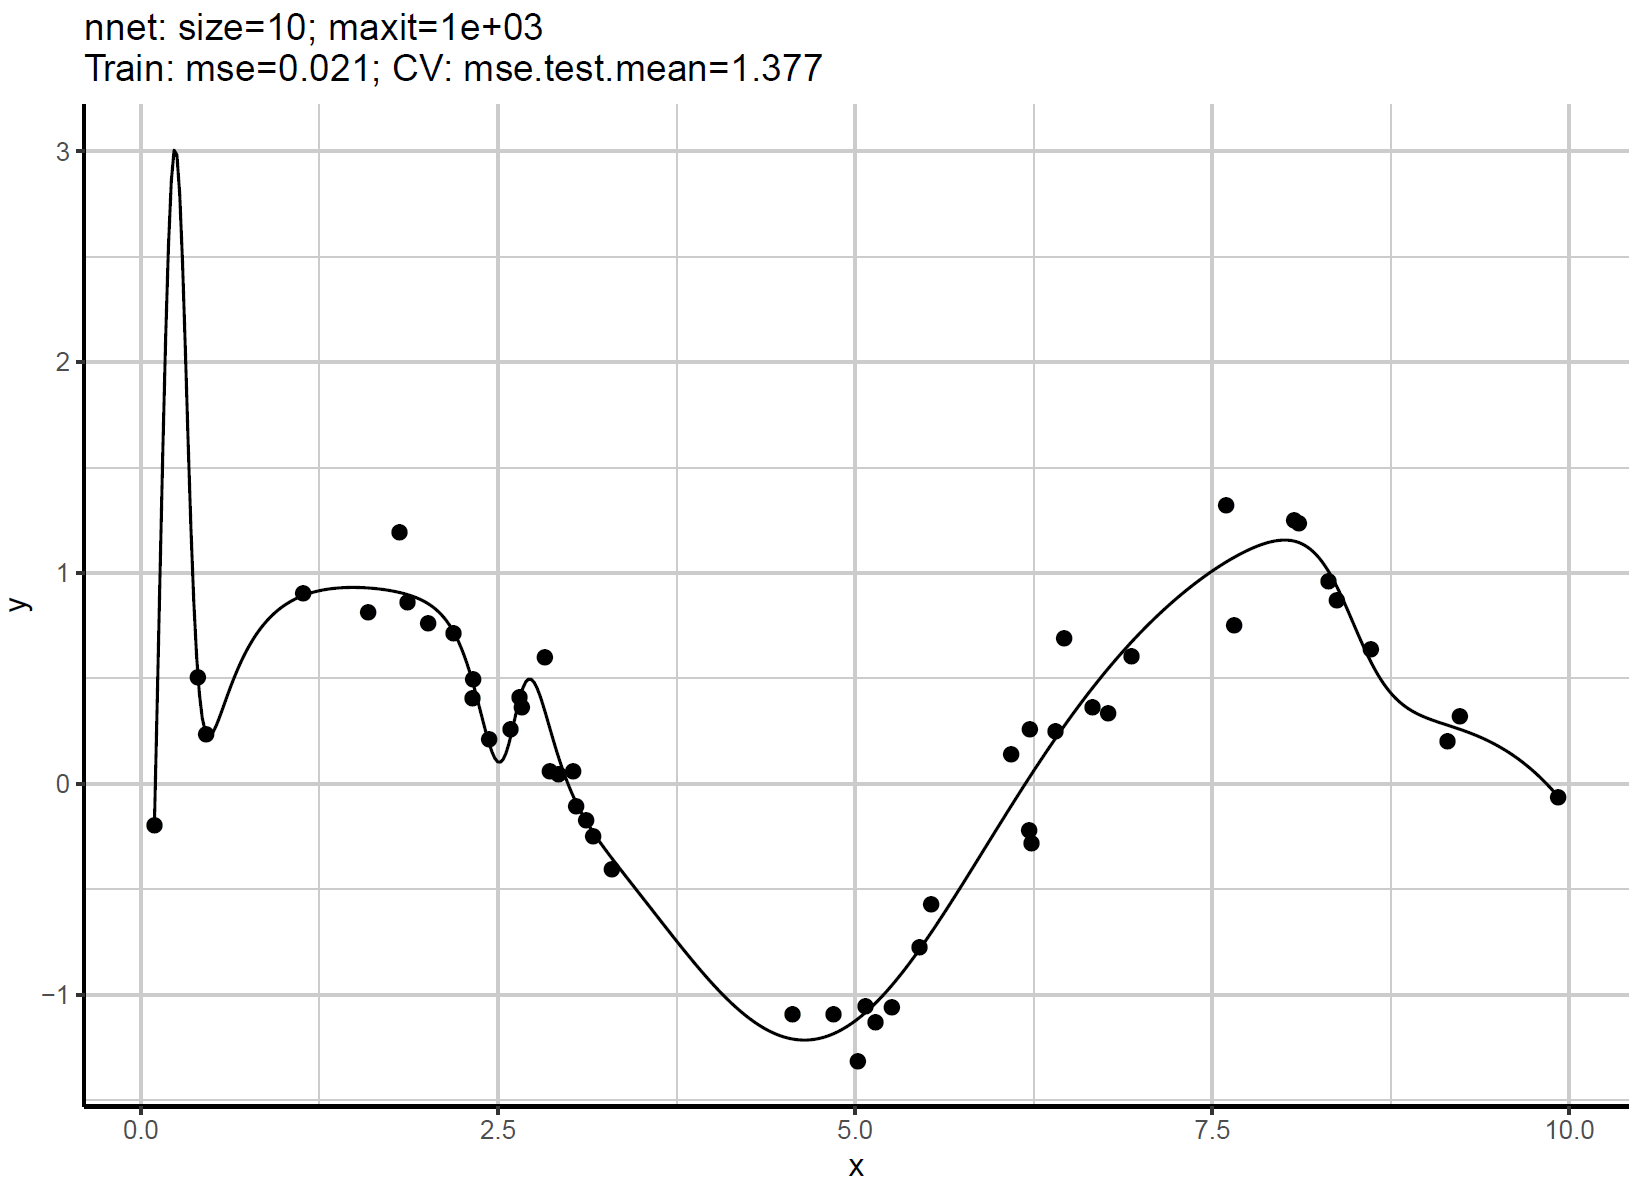
\includegraphics[width=0.9\textwidth]{plots/reg-n10.png}
\end{center}

}



\end{frame}
%%%%%%%%%%%%%%%%%%%%%%%%%%%%%%%%%%%%%%%%%%%%%%%%%%%%%%%%%%%%%%%%%%
%%%%%%%%%%%%%%%%%%%%%%%%%%%%%%%%%%%%%%%%%%%%%%%%%%%%%%%%%%%%%%%%%%
\begin{frame}{Classification: 500 training iterations}

\only<1>{

\begin{center}
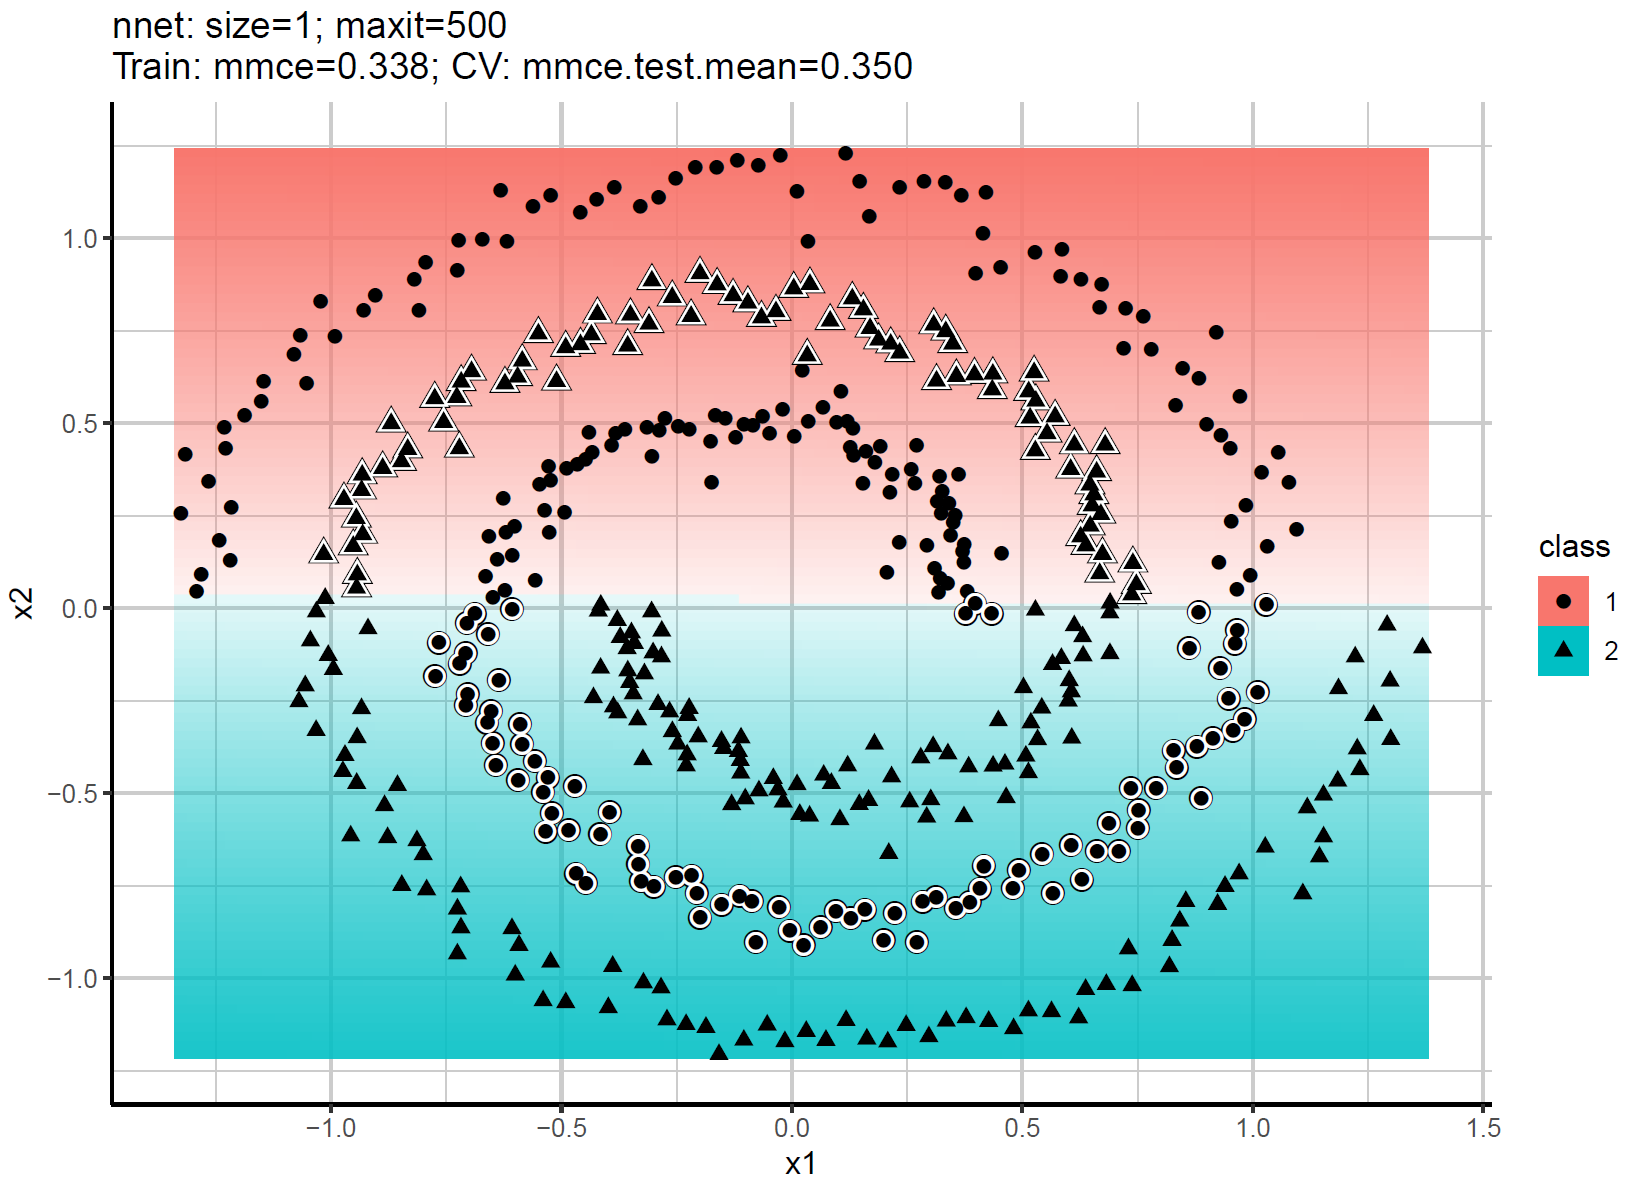
\includegraphics[width=0.9\textwidth]{plots/class-n1.png}
\end{center}

}

\only<2>{

\begin{center}
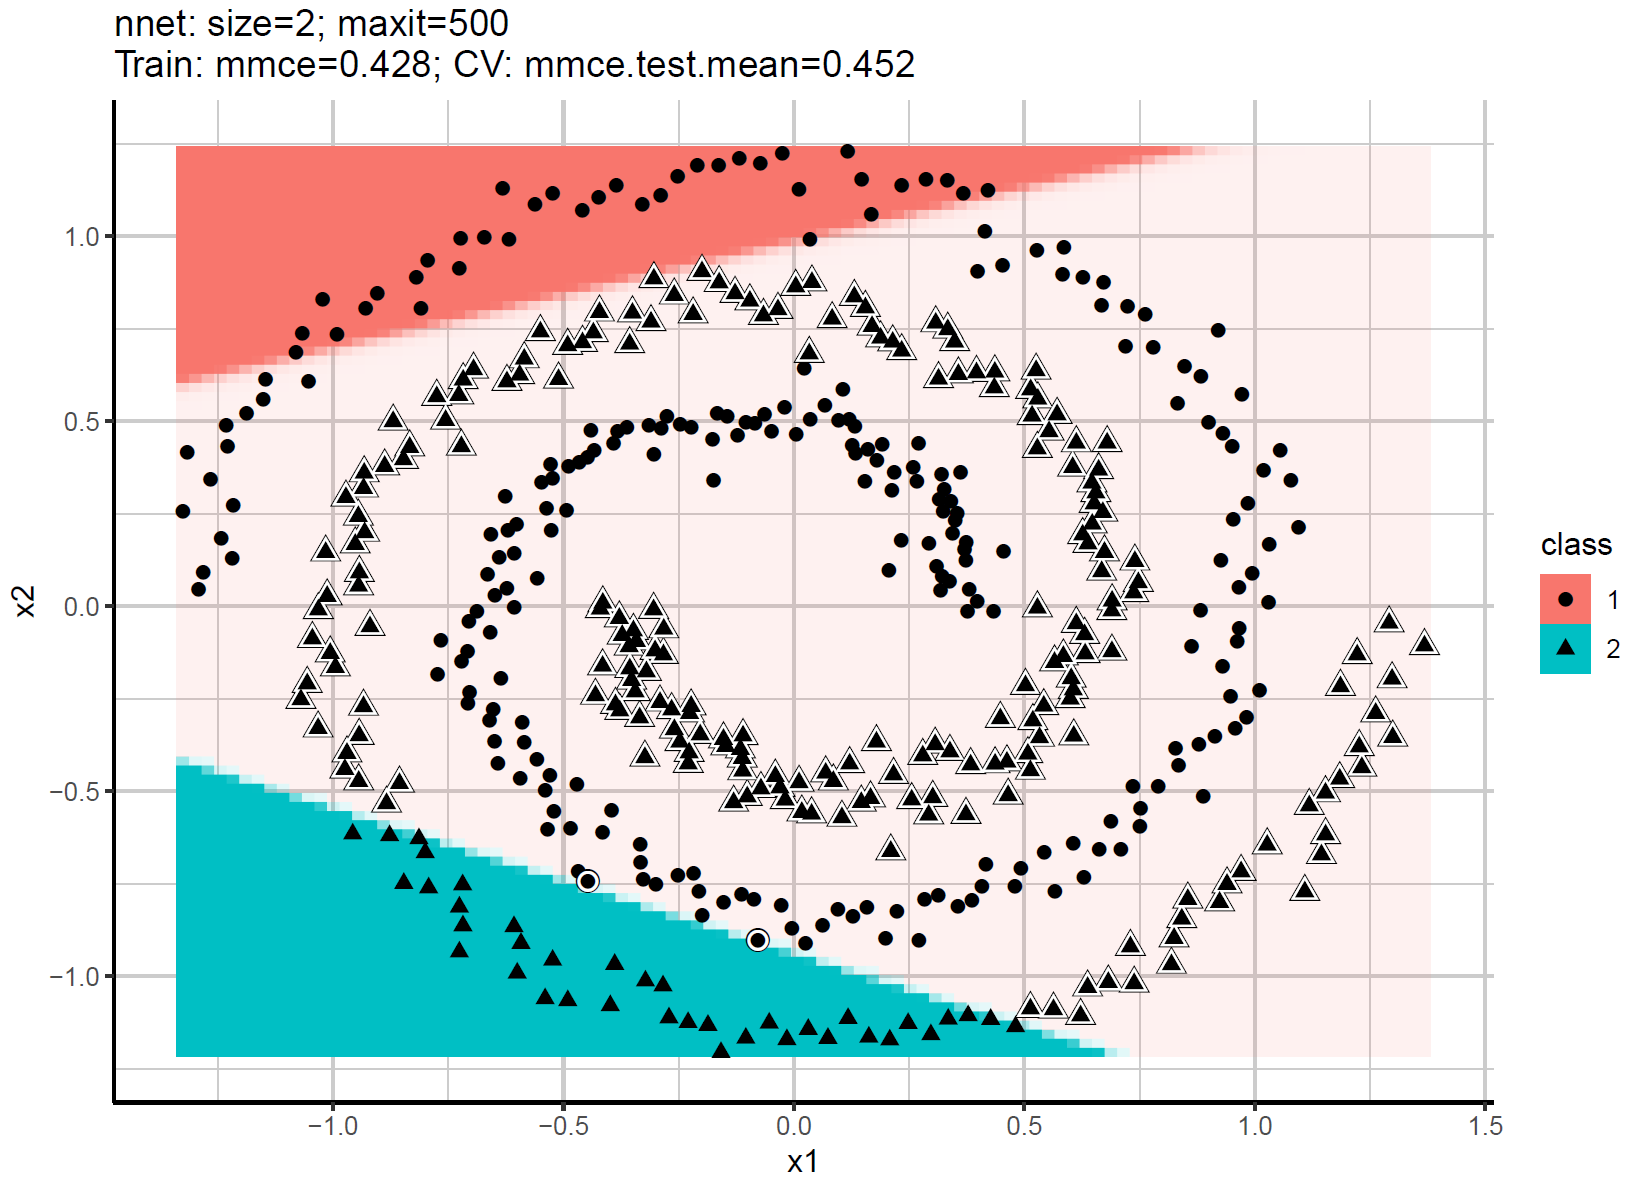
\includegraphics[width=0.9\textwidth]{plots/class-n2.png}
\end{center}

}

\only<3>{

\begin{center}
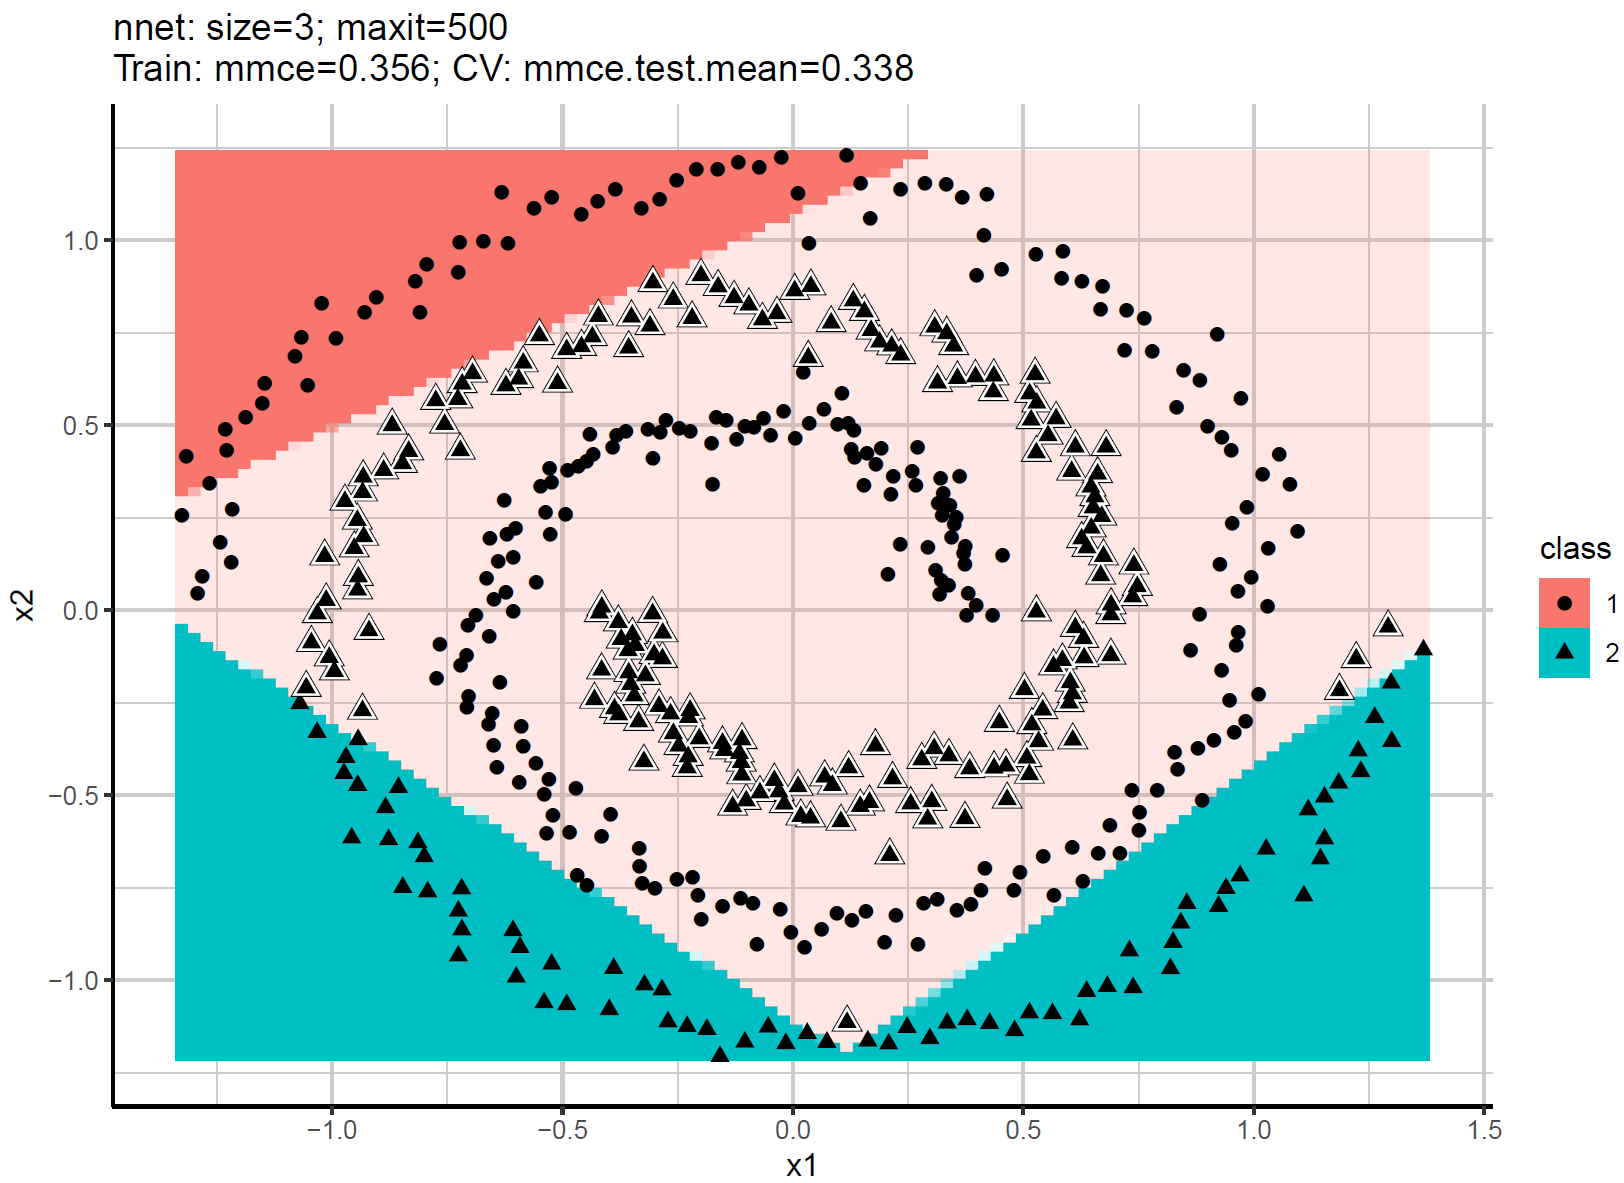
\includegraphics[width=0.9\textwidth]{plots/class-n3.png}
\end{center}

}

\only<4>{

\begin{center}
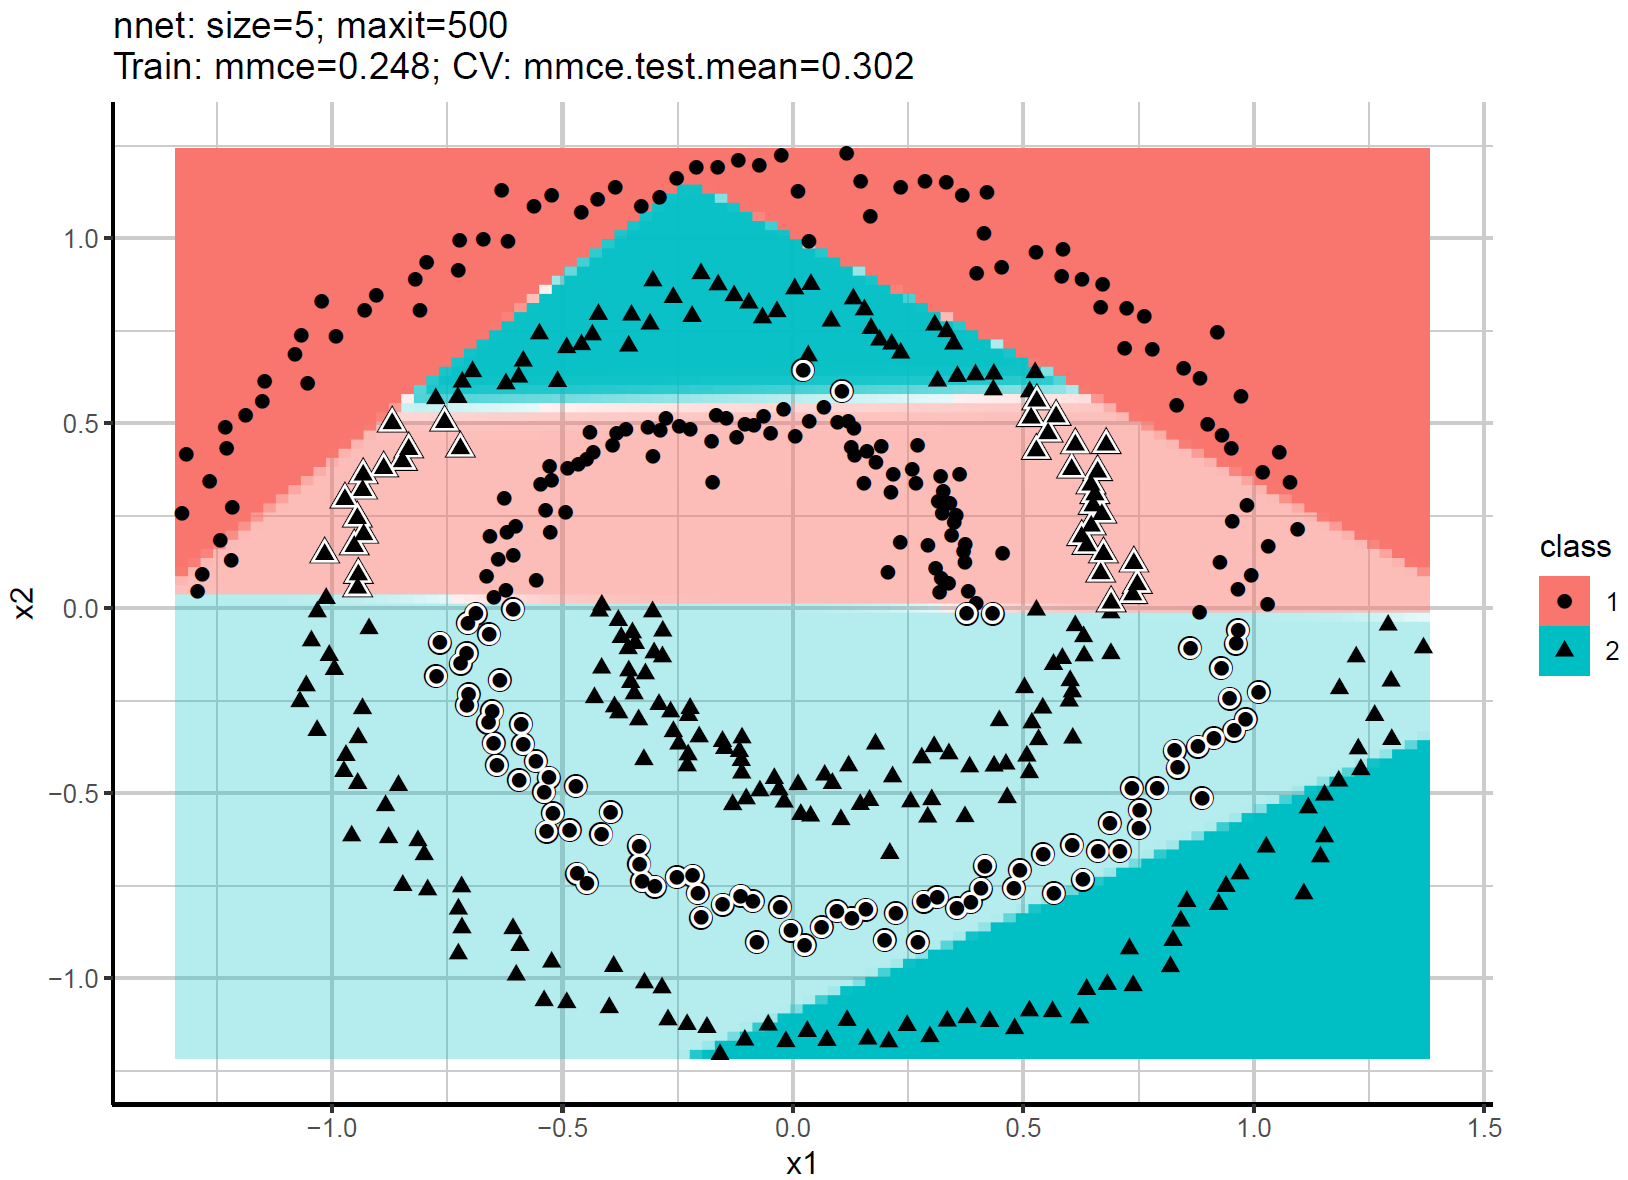
\includegraphics[width=0.9\textwidth]{plots/class-n5.png}
\end{center}

}

\only<5>{

\begin{center}
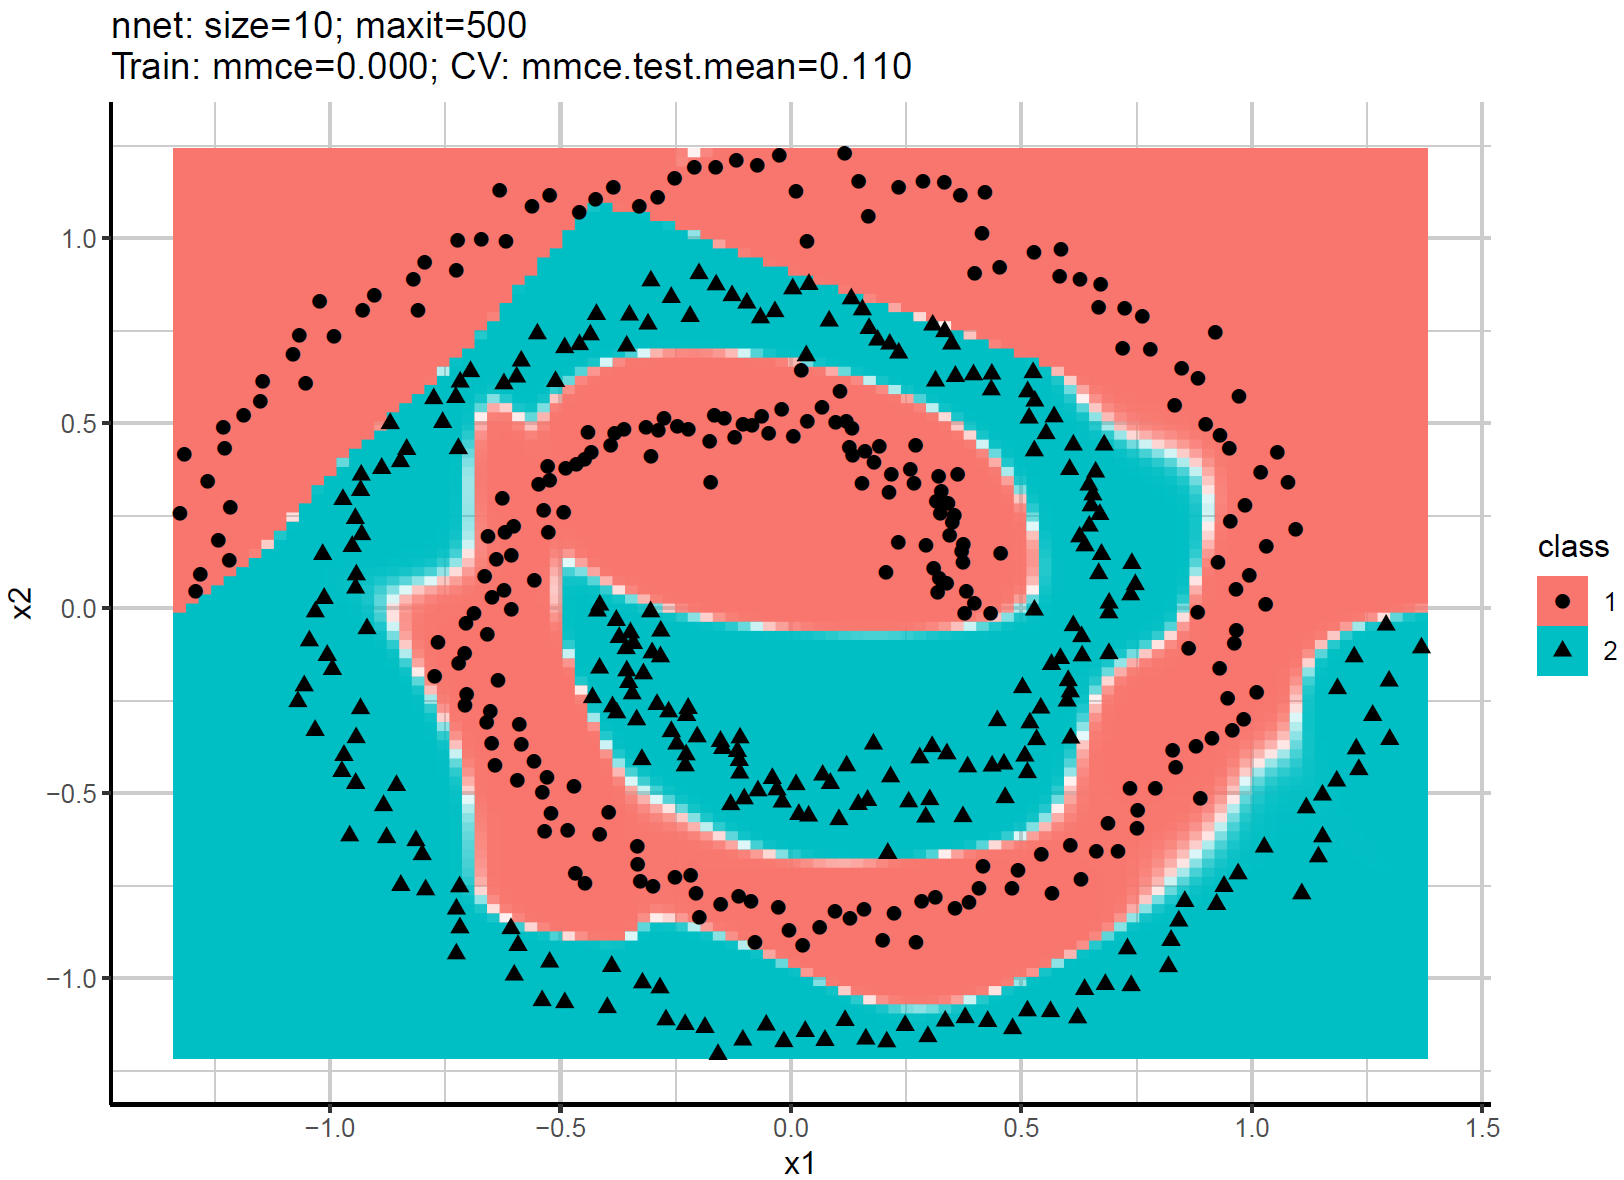
\includegraphics[width=0.9\textwidth]{plots/class-n10.png}
\end{center}

}

\only<6>{

\begin{center}
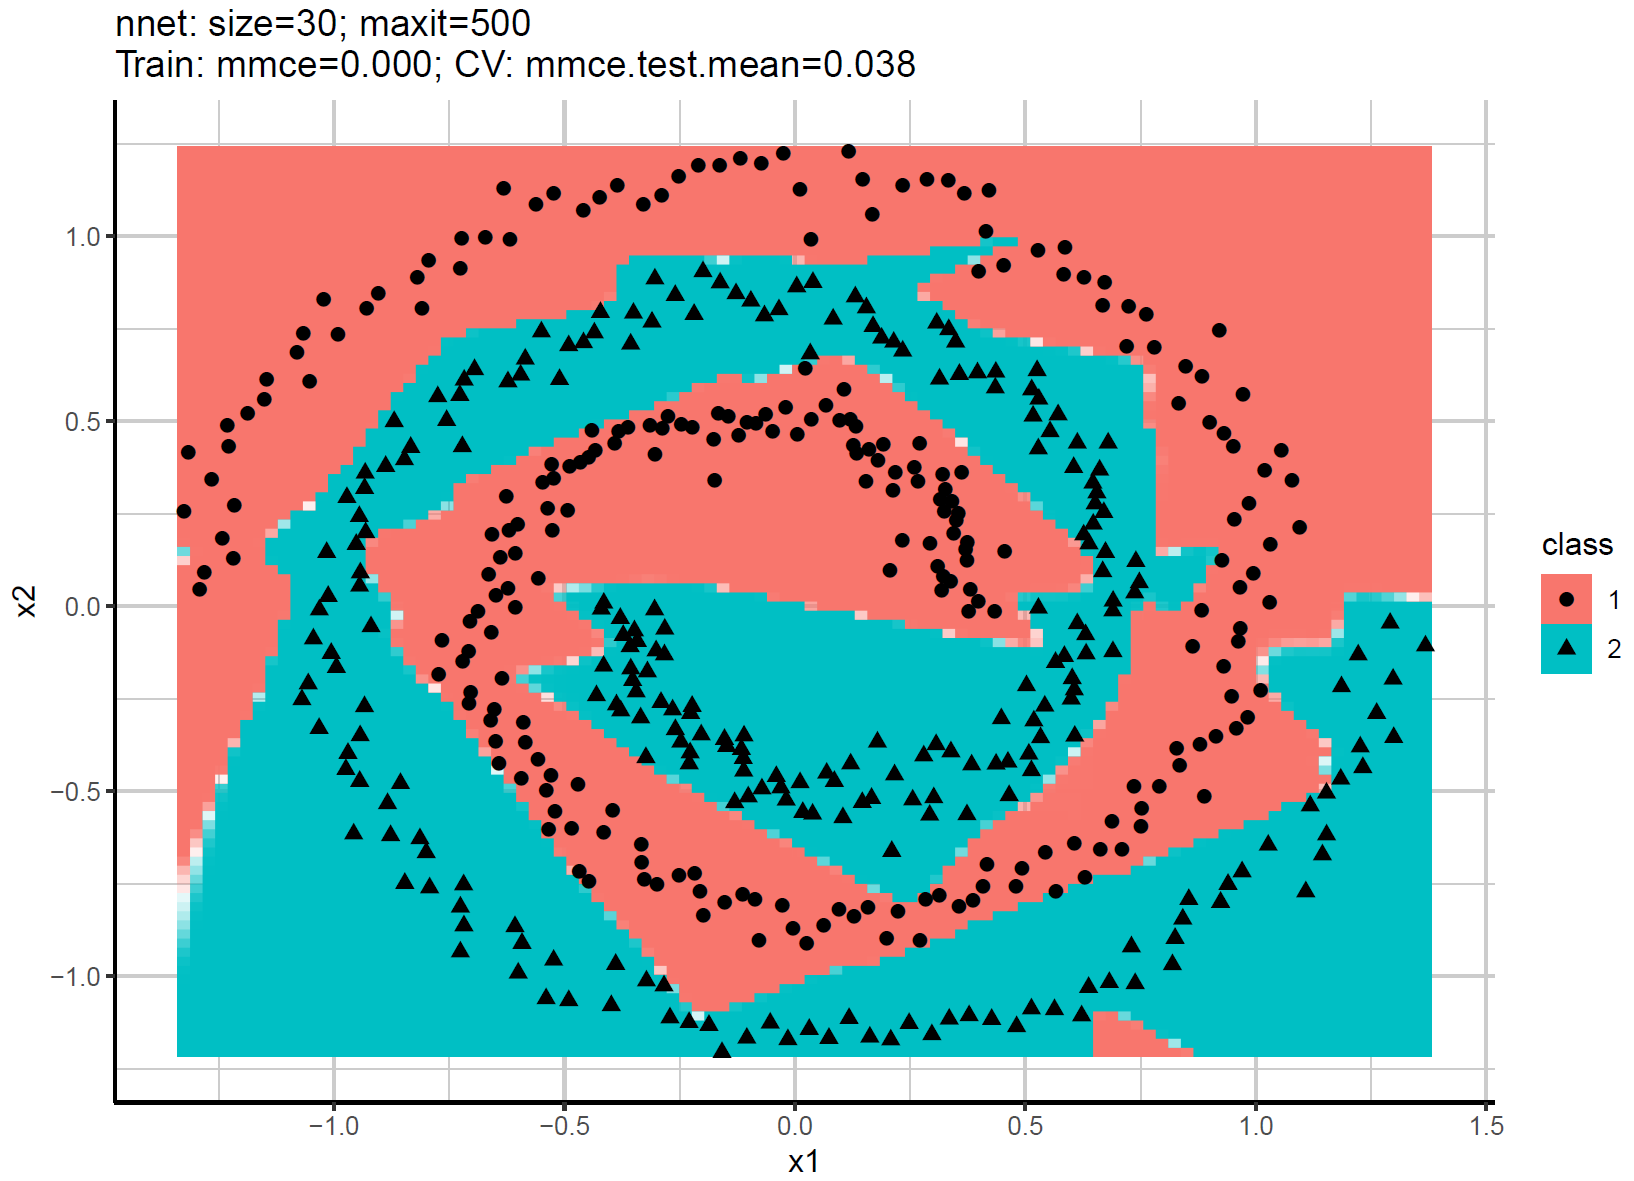
\includegraphics[width=0.9\textwidth]{plots/class-n30.png}
\end{center}

}

\only<7>{

\begin{center}
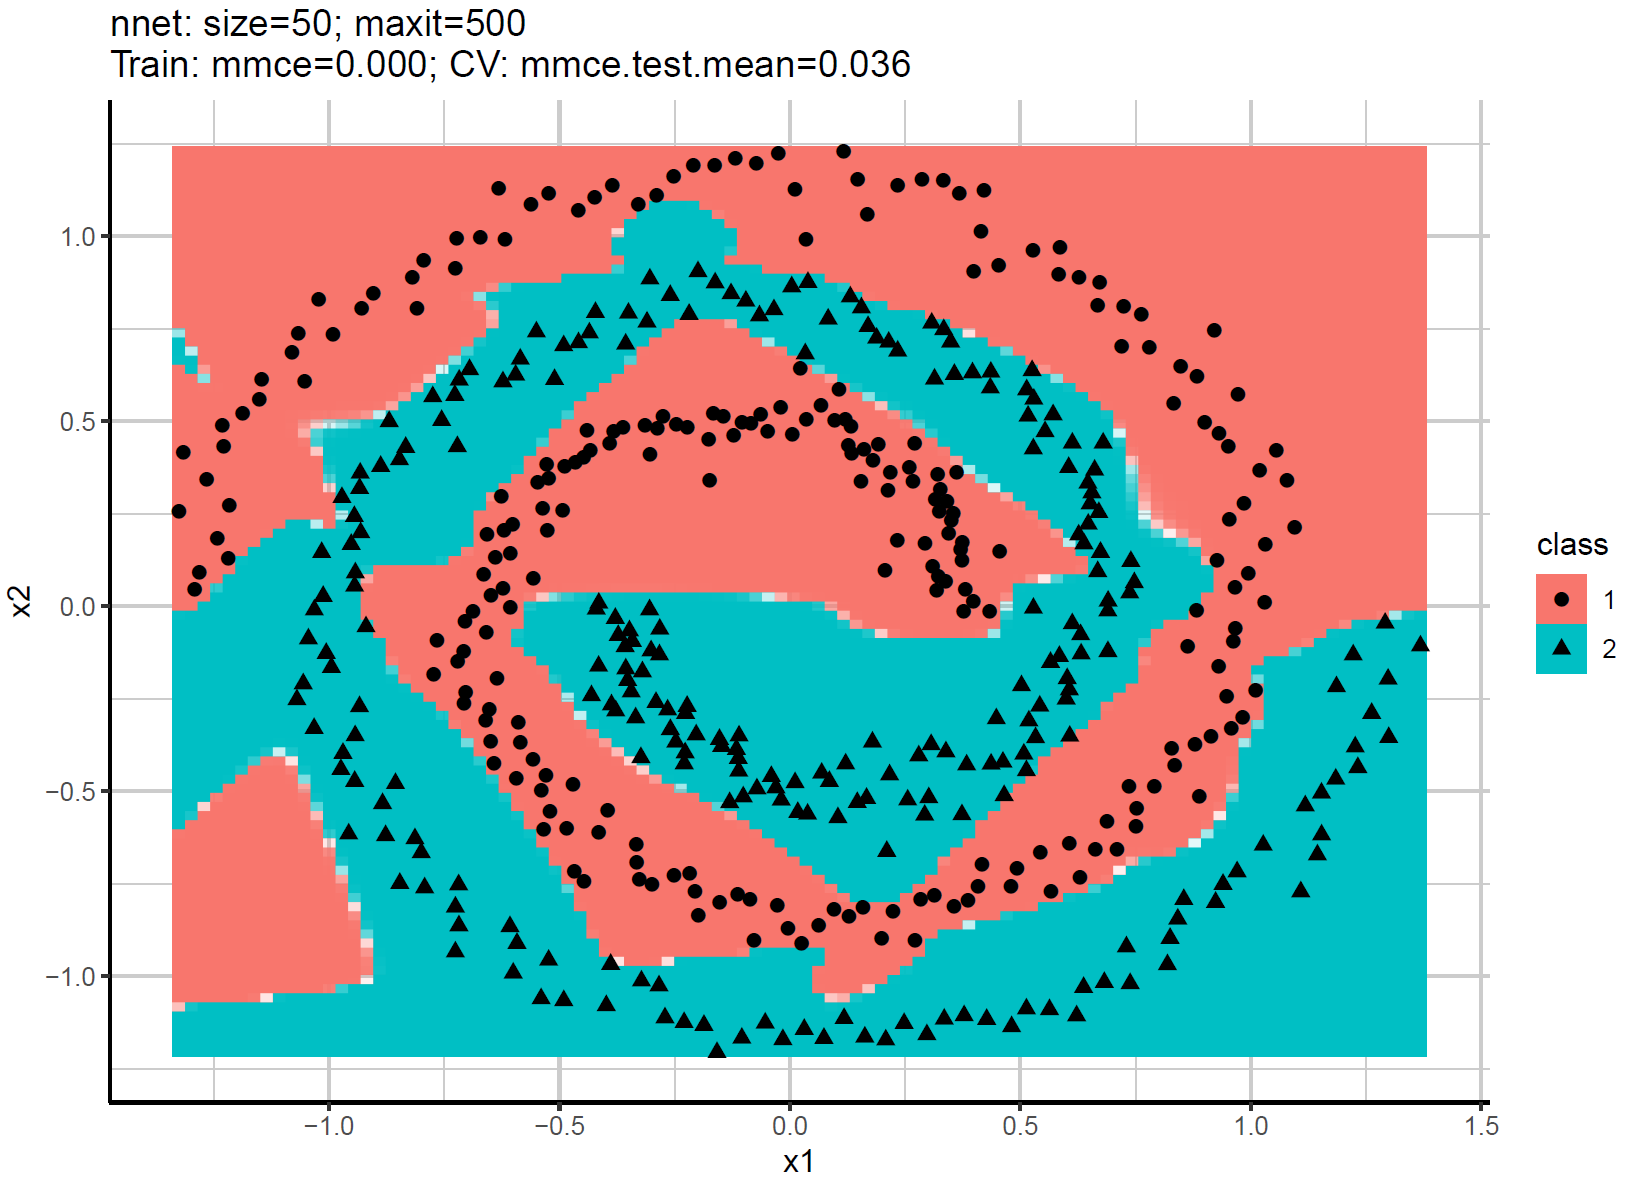
\includegraphics[width=0.9\textwidth]{plots/class-n50.png}
\end{center}

}

\end{frame}
%%%%%%%%%%%%%%%%%%%%%%%%%%%%%%%%%%%%%%%%%%%%%%%%%%%%%%%%%%%%%%%%%%
%%%%%%%%%%%%%%%%%%%%%%%%%%%%%%%%%%%%%%%%%%%%%%%%%%%%%%%%%%%%%%%%%%
% \begin{frame} {Representations}
%   \begin{itemize}
%     \item Regression and Classification examples
%   \end{itemize}
% \end{frame}
% 

\section{Single Hidden Layer Networks for Multi-Class Classification}

\begin{frame} {Multi-class Classification}
  \vspace{20mm}
  \begin{itemize}
    \item We have only considered regression and binary classification problems so far.
    \vspace{5mm}
    \item How can we get a neural network to perform multiclass classification?
  \end{itemize}
\end{frame}

\begin{frame} {Multi-class Classification}
  \begin{itemize}
    \item The first step is to add additional neurons to the output layer.
    \item Each neuron in the layer will represent a specific class (number of neurons in the output layer = number of classes).
    \begin{figure}
      \centering
      \scalebox{0.75}{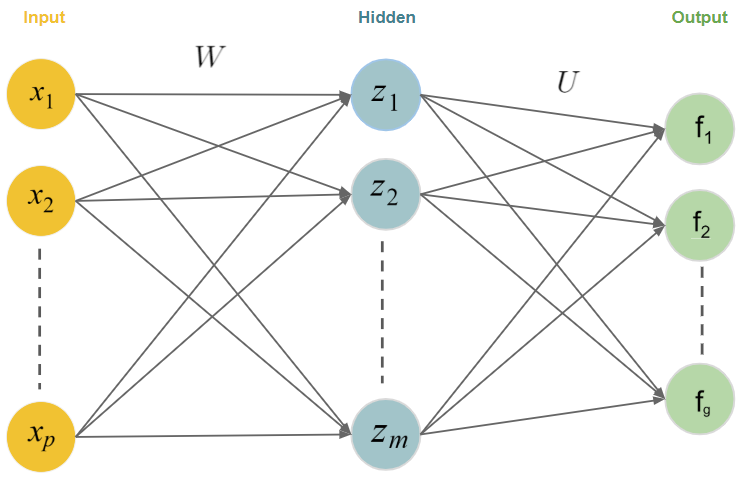
\includegraphics[width=10.2cm]{plots/neuralnet_new.png}}
        \caption{\footnotesize Structure of a single hidden layer, feed-forward neural network for g-class classification problems (bias term omitted).}
    \end{figure}
  \end{itemize}
\end{frame}

\begin{frame} {Multi-class Classification}
    \vspace{5mm}
    \begin{blocki}{Notation:}
    \item For $g$-class classification, $g$ output units: $$\mathbf{f} = (f_1, \dots, f_g)$$
    \vspace{4mm}
    \item $m$ hidden neurons $z_1, \dots, z_m$, with
    $$ z_j = \sigma(\Wmat_j^\top \xv), \quad j = 1,\ldots,m. $$
 %   \vspace{4mm}
    \item Compute linear combinations of derived features $z$:
    $$ f_{in,k} = \bm{U}_k^\top \hidz, \quad \hidz=(z_1,\dots, z_m)^\top, \quad k = 1,\ldots,g$$
  \end{blocki}
\end{frame}

\begin{frame} {Multi-class Classification}
  \begin{itemize}
    \item The second step is to apply a softmax activation function to the output layer.
    \vspace{4mm}
    \item This gives us a probability distribution over $g$ different possible classes:
    $$ f_{out,k} = \tau_k(f_{in,k}) = \frac{\exp(f_{in,k})}{\sum_{k'=1}^g\exp(f_{in,k'})}$$
    \vspace{2mm}
    \item This is the same transformation used in softmax regression!
    \vspace{4mm}
    \item Derivative $ \frac{\delta\tau(\mathbf{f}_{in})}{\delta \mathbf{f}_{in}} = \text{diag}(\tau(\mathbf{f}_{in})) - \tau(\mathbf{f}_{in}) \tau(\mathbf{f}_{in})^\top $
    \vspace{4mm}
    \item It is a \enquote{smooth} approximation of the argmax operation,
        so $\tau((1, 1000, 2)^\top) \approx (0, 1, 0)^\top$ (picks out 2nd element!).
  \end{itemize}
\end{frame}

\begin{frame} {Multi-class Classification: Example}
  \small{Forward pass (Hidden: Sigmoid, Output: Softmax).}
  \begin{figure}
    \centering
      \only<1>{\scalebox{0.95}{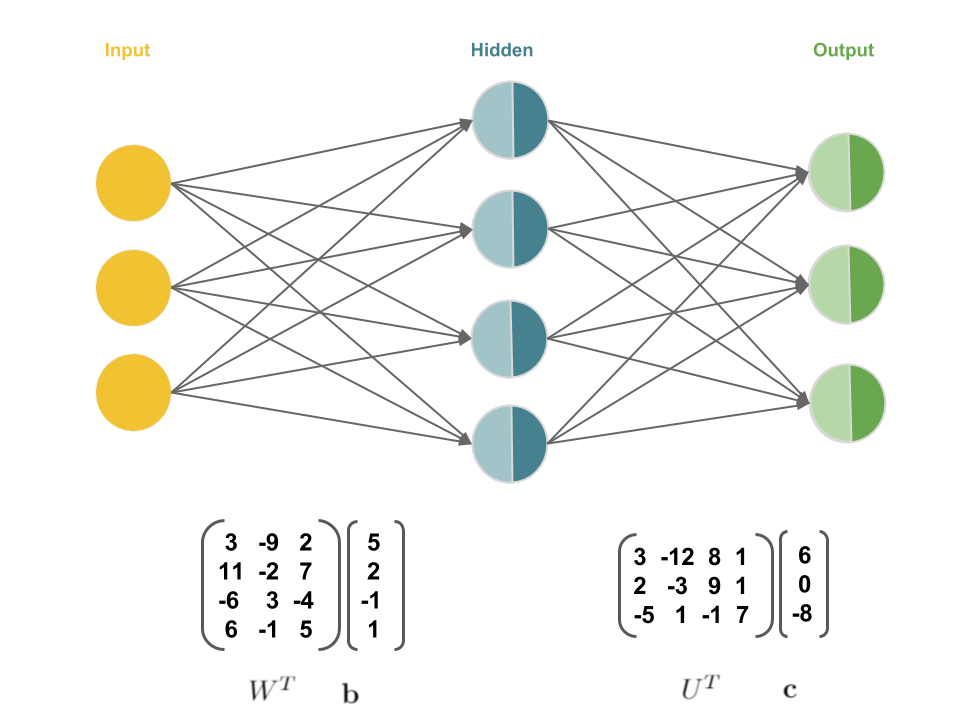
\includegraphics{plots/softie_one.png}}}
      \only<2>{\scalebox{0.95}{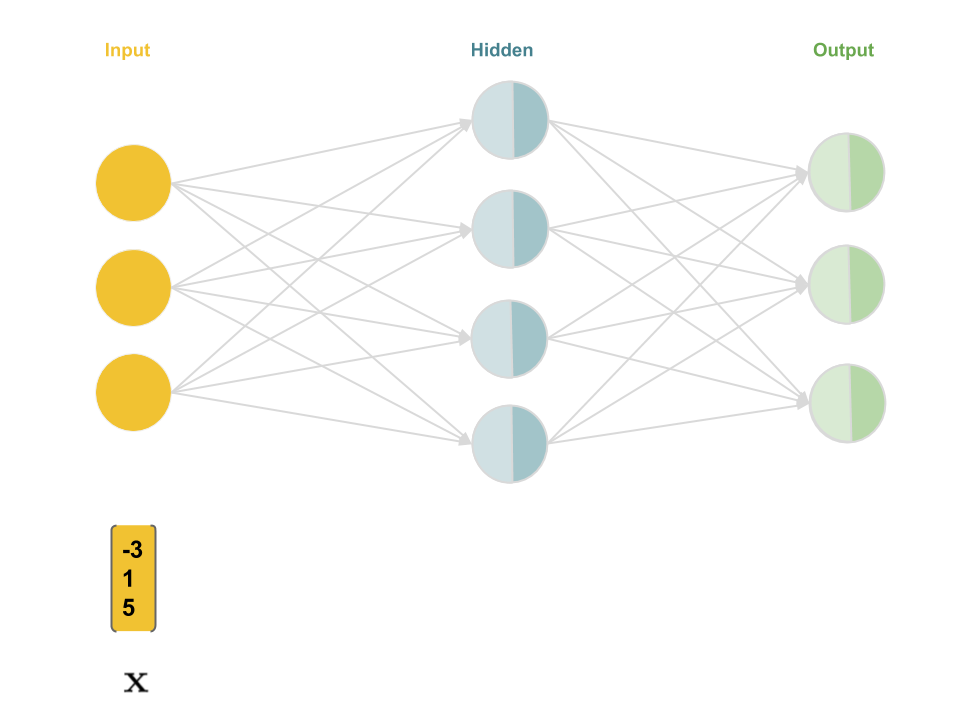
\includegraphics{plots/softie_two.png}}}
      \only<3>{\scalebox{0.95}{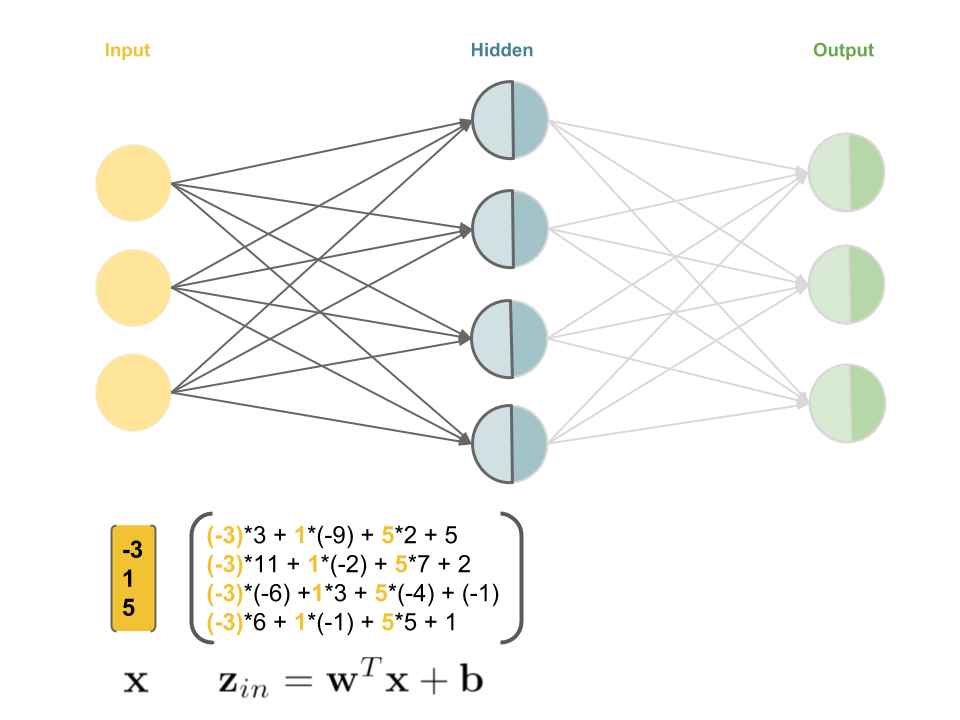
\includegraphics{plots/softie_three.png}}}
      \only<4>{\scalebox{0.95}{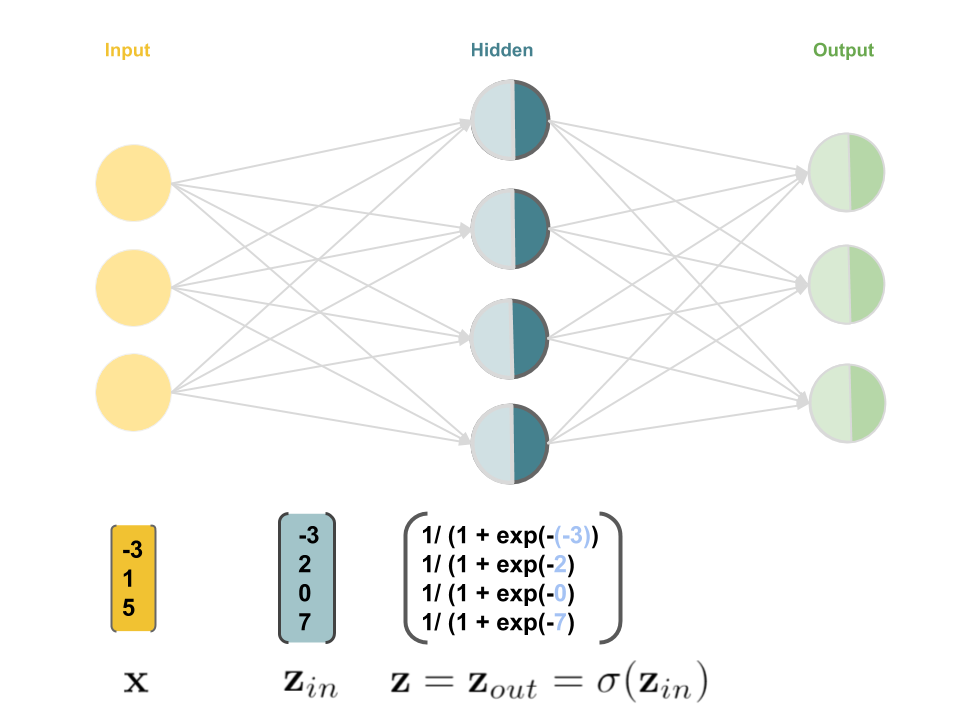
\includegraphics{plots/softie_four.png}}}
      \only<5>{\scalebox{0.95}{\includegraphics{plots/softie_five_a.png}}}
      \only<6>{\scalebox{0.95}{\includegraphics{plots/softie_five_b.png}}}
      \only<7>{\scalebox{0.95}{\includegraphics{plots/softie_six.png}}}
      \only<8>{\scalebox{0.95}{\includegraphics{plots/softie_seven.png}}}

  \end{figure}
\end{frame}

\begin{frame} {Softmax Loss}
  \begin{itemize}
    \vspace{5mm}
    \item The loss function for a softmax classifier is
    $$L(y, \fx) = - \sum_{k = 1}^g [y = k] \log \left( \frac{\exp(f_{in,k})}{\sum_{k'=1}^g\exp(f_{in,k'})}\right)$$
      where $[y = k] = \begin{cases} 1 & \text{ if } y = k \\
      0 & \text{ otherwise }
      \end{cases}$. 
    \vspace{5mm}
    \item This is equivalent to the cross-entropy loss when the label vector $\bm{y}$ is one-hot coded (e.g. $\mathbf{y} = (0,0,1,0)^\top$). 
    % $$
      % L(y, \fx) = - \sum_{k = 1}^g y_i \log \left( \frac{\exp(f_{in,k})}{\sum_{k'=1}^g\exp(f_{in,k'})}\right)
    % $$
    \item Optimization:  Again, there is no analytic solution. % Therefore, we use gradient descent.
  \end{itemize}
\end{frame}


%%%%%%%%%%%%%%%%%%%%%%%%%%%%%%%%%%%%%%%%%%%%%%%%%%%%%%%%%%%%%%%%%%
%%%%%%%%%%%%%%%%%%%%%%%%%%%%%%%%%%%%%%%%%%%%%%%%%%%%%%%%%%%%%%%%%%

%%%%%%%%%%%%%%%%%%%%%%%%%%%%%%%%%%%%%%%%%%%%%%%%
% XOR problem with sigmoid activation function %
%%%%%%%%%%%%%%%%%%%%%%%%%%%%%%%%%%%%%%%%%%%%%%%%
% \begin{vbframe}{XOR Problem 2}
%   \begin{eqnarray*}
%     z = \frac{1}{1+exp(-W^\topx+c)}
%     &=&
%     \begin{pmatrix}
%       -0.5 & 0.269 \\
%       0.731 & -0.5 \\
%       0.731 & -0.5 \\
%       0.881 & 0.731
%     \end{pmatrix} \\
%     &=&
%     \begin{pmatrix}
%       -1.038 \\
%       1.731 \\
%       1.731 \\
%       -0.581
%     \end{pmatrix}
%   \end{eqnarray*}
%   \begin{eqnarray*}
%     \hat{y} = \frac{1}{1+exp(-w^\topx+b)}
%     &=&
%     \begin{pmatrix}
%       0.26 \\
%       0.85 \\
%       0.85 \\
%       0.36
%     \end{pmatrix}
%   \end{eqnarray*}
% \end{vbframe}
%%%%%%%%%%%%%%%%%%%%%%%%%%%%%%%%%%%%%%%%%%%%%%%%%%%%%%%%%%%%%%%%%%
%%%%%%%%%%%%%%%%%%%%%%%%%%%%%%%%%%%%%%%%%%%%%%%%%%%%%%%%%%%%%%%%%%
\begin{vbframe}{Single Hidden Layer Networks: Summary}
  \begin{itemize}
    \item We have seen that neural networks are far more flexible than linear models. Neural networks with a single hidden layer are able to approximate any continuous function.
    \item Yet, in reality, there is no way to make full use of the universal approximation property. The learning algorithm will usually not find the best possible model. At best it finds a locally optimal model. 
    \item The XOR example showed us how neural networks extract features to transform the space and actually learn a kernel (learn a representation).
    \item Neural networks can perfectly fit noisy data. Thus, neural networks are endangered to over-fit. This is particularly true for a model with a huge hidden layer.
    \item Fitting neural networks with sigmoidal activation function is nothing else but fitting many weighted logistic regressions!
  \end{itemize}
\end{vbframe}

\section{Multi-Layer Feedforward Neural Networks}

\begin{vbframe}{Feedforward neural networks}
  \begin{itemize}
    \vspace{15mm}
    \item We will now extend the model class once again, such that we allow an arbitrary amount of $l$ (hidden) layers.
    \vspace{5mm}
    \item The general term for this model class is (multi-layer) \textbf{feedforward networks} (inputs are passed through the network from left to right, no feedback-loops are allowed)
    % \begin{itemize}
    %   \item If $h = 0$, i.e. we only have input and output layer, the model is called \textbf{single layer perceptron}
    %   \item If we have $h > 0$ layers, i.e. at least on hidden layer, then the model class is also called \textbf{multi layer perceptron} 
    % \end{itemize}
  \end{itemize}
\framebreak
  \begin{itemize}
%     \item We can characterize those models by the following chain structure: $$f(x) = g(f_{(k)}(f_{(k-1)}(f_{(k-2)}(\ldots(f_{(1)}(x))\ldots)$$ where $f_{(1)}$ corresponds to the first and $f_{(k)}$ to the last layer of the network.
%     \item We can characterize those models by the following chain structure: $$f(\xv) = \tau(\sigma^{(k)}(\sigma^{(k-1)}(\sigma^{(k-2)}(\ldots(\sigma^{(1)}(W^{(1)T}\xv + \biasb^1)))$$ where $\sigma^{(1)}$ corresponds to the first and $\sigma^{(k)}$ to the last layer of the network.
%   \end{itemize}
% \framebreak
%   \begin{itemize}
%     \item We will now extend the model class once again, such that we allow an arbitrary amount of $K$ layers.
%       \begin{itemize}
%         \item For more than one hidden layer, we call such graphs deep feedforward networks.
%       \end{itemize}
    % \item We can characterize those models by the following chain structure: $$f(\xv) = \tau(\sigma^{(K)}(\sigma^{(K-1)}(\sigma^{(K-2)}(\ldots(\sigma^{(1)}(W^{(1)T}\xv + \biasb^{(1)})))$$ where $\sigma^{(1)}$ corresponds to the first and $\sigma^{(k)}$ to the last (hidden) layer of the network.
        \item We can characterize those models by the following chain structure: $$f(\xv) = \tau \circ \phi \circ \sigma^{(l)} \circ \phi^{(l)} \circ \sigma^{(l-1)} \circ \phi^{(l-1)} \circ \ldots \circ \sigma^{(1)} \circ \phi^{(1)}$$ where $\sigma^{(i)}$ and $\phi^{(i)}$ are the activation function and the weighted sum of hidden layer $i$, respectively. $\tau$ and $\phi$ are the corresponding components of the output layer.

%(W^{(1)T}\xv + \biasb^{(1)})

    \vspace{5mm}
    \item Each hidden layer has: 
      \begin{itemize}
        \vspace{2mm}
        \item an associated weight matrix $\Wmat^{(i)}$, bias $\biasb^{(i)}$ and activations $\hidz^{(i)}$ for $i \in \{ 1 \ldots l\}$
        \vspace{2mm}
        \item $\hidz^{(i)} = \sigma^{(i)}(\phi^{(i)}) = \sigma^{(i)}(\Wmat^{(i)T}\hidz^{(i - 1)} + \biasb^{(i)})$ , where $\hidz^{(0)} = \xv$.
      \end{itemize}
    \vspace{5mm}
    \item Again, without non-linear activations in the hidden layers, the network can only learn linear decision boundaries.
  \end{itemize}
\framebreak
  \lz
  \begin{figure}
    \centering
      \includegraphics[width=10.5cm]{plots/deepneuralnet_new.png}
      \caption{Structure of a deep neural network with $l$ hidden layers (bias terms omitted).}
  \end{figure}
% \framebreak
%   \begin{itemize}
%     \item Mathematically, we observe the following mappings: 
%   \end{itemize}
%   \begin{eqnarray*}
%     &f_1(x):& \R^P \to \R^{M_1} \\
%     &f_2(f_1):& \R^{M_1} \to \R^{M_2} \\
%     &...& \\
%     &f_H(..):& \R^{M_{H-1}} \to \R^{M_H}, \ \forall h = 2,\dots,H \\
%     &g(..):& \R^{M_H} \to \R^{K}
%   \end{eqnarray*}
%   \begin{figure}
%     \centering
%       \includegraphics[width=5cm]{plots/deepneuralnet.png}
%   \end{figure}
\end{vbframe}  

% \begin{frame} {Deep feedforward networks: Matrix}
%   \begin{itemize}
%     \item Each layer has an associated weight matrix W
%     \item and hidden activations z1, z2,z3,
%     
%   \end{itemize}
% \end{frame}
% 
% \begin{frame} {Why deep}
%   \begin{itemize}
%     \item The best way to think of these layers is as representing hierarchies of features where earlier layers represent the simpler features and later layers represent more complex features.
%     \item Edges, nose, face
%   \end{itemize}
% \end{frame}

% \begin{frame} {DL}
%   \item A whole bunch of linear layers is just a linear layer
% \end{frame}
% 
% \begin{frame} {DL}
%   \item Not only is DL a way to automate representation, it is a clever way of doing it.
%   \item Bloody good prior
%   \item That's why our brains are organized in a similar way
%   \item NFL theorem
%   \item Why depth matters
% \end{frame}
% 
% \begin{frame} {DL}
%   \item Why depth matters: Empirical
% \end{frame}
% 
% \begin{frame} {DL}
%   \item Why depth matters: Theoretical
% \end{frame}

%%%%%%%%%%%%%%%%%%%%%%%%%%%%%%%%%%%%%%%%%%%%%%%%%%%%%%%%%%%%%%%%%%
\begin{frame} {Feedforward neural networks: Example}
  \begin{figure}
    \centering
\only<1>{\scalebox{0.95}{\includegraphics{plots/deepnet_one.png}}}
\only<2>{\scalebox{0.95}{\includegraphics{plots/deepnet_two.png}}}
\only<3>{\scalebox{0.95}{\includegraphics{plots/deepnet_three.png}}}
\only<4>{\scalebox{0.95}{\includegraphics{plots/deepnet_four.png}}}
\only<5>{\scalebox{0.95}{\includegraphics{plots/deepnet_five.png}}}
\only<6>{\scalebox{0.95}{\includegraphics{plots/deepnet_six.png}}}
\only<7>{\scalebox{0.95}{\includegraphics{plots/deepnet_seven.png}}}
\only<8>{\scalebox{0.95}{\includegraphics{plots/deepnet_eight.png}}}
\only<9>{\scalebox{0.95}{\includegraphics{plots/deepnet_nine.png}}}
\only<10>{\scalebox{0.95}{\includegraphics{plots/deepnet_ten.png}}}
\only<11>{\scalebox{0.95}{\includegraphics{plots/deepnet_eleven.png}}}
\only<12>{\scalebox{0.95}{\includegraphics{plots/deepnet_twelve.png}}}
  \end{figure}
\end{frame}

%%%%%%%%%%%%%%%%%%%%%%%%%%%%%%%%%%%%%%%%%%%%%%%%%%%%%%%%%%%%%%%%%%
\begin{vbframe}{Why add more layers?}
\begin{itemize}
  \item Multiple layers allow for the extraction of more and more abstract representations.
\end{itemize}
  \begin{figure}
    \centering
      \includegraphics[width=4cm]{plots/hierachicalRepresentations.png}
      \caption{Y. Bengio,  Learning Deep Architectures for AI, Foundations and trends® in Machine Learning, 2009}
  \end{figure}
\end{vbframe}


\begin{vbframe}{Why add more layers?}
\begin{itemize}
  \item Each layer in a feed-forward neural network adds its own degree of non-linearity to the model.
\end{itemize}
  \begin{figure}
    \centering
      \includegraphics[width=10.5cm]{plots/folding}
      \caption{An intuitive, geometric explanation of the exponential advantage of deeper networks formally (Mont\'{u}far et al. (2014)).}
  \end{figure}
\end{vbframe}
%%%%%%%%%%%%%%%%%%%%%%%%%%%%%%%%%%%%%%%%%%%%%%%%%%%%%%%%%%%%%%%%%%

\section{Deep Learning}

\begin{vbframe}{Deep neural networks}

  \begin{itemize}
    \item Neural networks today can have dozens or even hundreds of hidden layers. The greater the number of layers, the "deeper" the network. 
    \item Historically, deep neural networks were very challenging to train for several reasons.
    \item For one thing, the use of sigmoid activations (such as logistic sigmoid and tanh) significantly slowed down training due to a phenomenon known as \enquote{vanishing gradients}. The introduction of the ReLU activation largely solved this problem.
    \item Additionally, training deep neural networks on CPUs was too slow to be practical. Switching over to GPUs (Graphics Processing Units) cut down training time by more than an order of magnitude.
    \item Another reason neural networks were not popular until the late '00s is that when dataset sizes are small, other models (such as SVMs) and techniques (such as feature engineering) outperform them. 
    \item Therefore, the availability of large datasets (such as ImageNet) and novel architectures that are capable to handle even complex tensor-shaped data (e.g. CNNs for image data), significantly faster hardware, and equally better optimization and regularization methods made it feasible to successfully implement deep neural networks in the last decade.
    \item An increase in depth often translates to an increase in performance on a given task. 
    \item State-of-the-art neural networks, however, are much more sophisticated than the simple architectures we have encountered so far. (Stay tuned!)
    \item The term "\textbf{deep learning}" encompasses all of these developments and refers to the field as a whole.
  \end{itemize}
\end{vbframe}


% \begin{frame} {Why now and not earlier?(Can delete)}
% 
% %https://alisha17.github.io/machine-learning/2017/12/15/benchmarks.html
% \begin{figure}
%     \centering
%       \scalebox{0.75}{\includegraphics{plots/whynow_gpu.jpg}}
%       \tiny{\\Source: dl4j}
%   \end{figure}
% \end{frame}



%%%%%%%%%%%%%%%%%%%%%%%%%%%%%%%%%%%%%%%%%%%%%%%%%%%%%%%%%%%%%%%%%%%%%%%%%%%%%%%%%%%%%%%%%%%%%%%%%%%
%%%%%%%%%%%%%%%%%%%%%%%%%%%%%%%%%%%%%%%%%%%%%%%%%%%%%%%%%%%%%%%%%%
% \begin{vbframe}{Number of parameters in a neural network}
%   \begin{itemize}
%     \item For a fix input and output, a neural network has 
%     $$M_1 \cdot M_2 \cdot ... \cdot M_H$$ 
%     parameters in its hidden layers.
%     \lz
%     \item or just
%     $$M^H$$ 
%     for the same amount of neurons in each layer (note that we omitted bias terms).
%   \end{itemize}
% \framebreak
% <<echo=FALSE, fig.height=5.5>>=
% library(ggplot2)
% logfun = function(v, s) {
%   v^s
% }
% x = seq(0, 10, 0.1)
% stretch = c(2, 3, 4)
% y = sapply(stretch, function(s) {
%   sapply(x, logfun, s = s)
% })
% 
% df = data.frame(y = as.vector(y), 
%   x = rep(x, length(stretch)),
%   s = as.factor(rep(stretch, each = length(x))))
% 
% hl = ggplot(df, 
%   aes(x = x, y = y, color = s)) + 
%   geom_line(size = 1) +
%   scale_y_continuous(name = "# parameters") +
%   scale_x_continuous(labels = function (x) floor(x), 
%     name = "# neurons in each hidden layer") +
%   theme(axis.title = element_text(size = 14L, 
%     face = "bold"),
%     plot.margin = unit(c(0, 0, 0, 0), "cm"), 
%     legend.position = c(0.25, 0.78), 
%     legend.background = element_rect(fill="transparent")) +
%   labs(colour = "number of\nhidden layers") 
% 
% hl
% @
% \end{vbframe}
%%%%%%%%%%%%%%%%%%%%%%%%%%%%%%%%%%%%%%%%%%%%%%%%%%%%%%%%%%%%%%%%%%
%%%%%%%%%%%%%%%%%%%%%%%%%%%%%%%%%%%%%%%%%%%%%%%%%%%%%%%%%%%%%%%%%%
% \begin{vbframe}{Initializing of the parameters}
%   \begin{itemize}
%     \item This topic is basically part of neural network optimization and not yet fully understood.
%     \item The choice of initial weights strongly influences the speed of convergence as well as optimality (ending up in a local or global minima).
%     \lz
%     \item Common strategies for weight initialization are:
%       \begin{itemize}
%         \item Drawing from a standard normal distribution.
%         \item Drawing from an uniform distribution with zero mean and sqrt(number of parameters) (LeCun et al. (1998)).
%         \item Unsupervised layerwise pre-training (Hinton and Salakhutdinov (2006)).
%       \end{itemize}
%   \end{itemize}
% \end{vbframe}
% %%%%%%%%%%%%%%%%%%%%%%%%%%%%%%%%%%%%%%%%%%%%%%%%%%%%%%%%%%%%%%%%%%
%%%%%%%%%%%%%%%%%%%%%%%%%%%%%%%%%%%%%%%%%%%%%%%%%%%%%%%%%%%%%%%%%%
% \begin{vbframe}{Introduction to MXNet}
%   \begin{itemize}
%     \item Open-source deep learning framework written in C++ and cuda (used by Amazon for their Amazon Web Services)
%     \item Scalable, allowing fast model training
%     \item Supports flexible model programming and multiple languages (C++, Python, Julia, Matlab, JavaScript, Go, \textbf{R}, Scala, Perl)
%     \item Installation instructions for different operating systems: \url{http://mxnet.io/get_started/install.html}
%   \end{itemize}
% \end{vbframe}
% %%%%%%%%%%%%%%%%%%%%%%%%%%%%%%%%%%%%%%%%%%%%%%%%%%%%%%%%%%%%%%%%%%
% %%%%%%%%%%%%%%%%%%%%%%%%%%%%%%%%%%%%%%%%%%%%%%%%%%%%%%%%%%%%%%%%%%
% \begin{vbframe}{Kaggle challenge digit recognizer}
%     \begin{itemize}
%       \item The MNIST database is a large database of handwritten digits (black and white) that is commonly used for benchmarking various image processing algorithms.
%       \item It is a good database for people who want to try learning techniques and pattern recognition methods on real-world data while spending minimal efforts on preprocessing and formatting.
%       \item  There have been a number of scientific papers on attempts to achieve the lowest error rate. One paper, using a hierarchical system of convolutional neural networks (chapter 4), manages to get an error rate of only 0.23 percent.
%     \end{itemize}
% \framebreak
%   \begin{figure}
%     \centering
%       \includegraphics[width=10cm]{plots/mnist.png}
%       \caption{Snipped from the mnist data set (LeCun and Cortes (2010)).}
%   \end{figure}
%   \begin{itemize}
%     \item 70k image data of handwritten digits with $28 \times 28$ pixels.
%     \item Classification task with 10 classes (e.g. 0, 1, 2, ..., 9).
%     \item In R: the darch package gives an easy option to access the data.
%     \item[] ...but for our example, we use another source with a more difficult train/test split.
%   \end{itemize}
% \framebreak
%   \begin{itemize}
%     \item Since competing with others is more fun, we dare ourselves to face the mnist kaggle challenge.
%     \item Therefor, we download the data sets (train.csv and test.csv) from \url{https://www.kaggle.com/c/digit-recognizer/data}.
%     \item We obtain $42.000$ images for training and $28.000$ for testing.
%   \end{itemize}
% %%%%%%%%%%%%%%%%%%%%%%%%%%%%%%%%%%%%%%%%%%%%%%%%%%%%%%%%%%%%%%%%%%%%%%%%
% %%%%%%%%%%%%%%%%%%%%%%%%%%%%%% READ ME!!! %%%%%%%%%%%%%%%%%%%%%%%%%%%%%%
% %%%%%%%%%%%%%%%%%%%%%%%%%%%%%%%%%%%%%%%%%%%%%%%%%%%%%%%%%%%%%%%%%%%%%%%%
% % The following slides include lots of code chunks which have been     %
% % temporarily disabled (eval = FALSE, echo = FALSE) and replaced by    %
% % screenshots of the corresponding outputs (to maintain colorization). %
% % Else, one would need a working version of mxnet (and a fast CPU/GPU) %
% % to compile the code in a finite amount of time.                      %
% %%%%%%%%%%%%%%%%%%%%%%%%%%%%%%%%%%%%%%%%%%%%%%%%%%%%%%%%%%%%%%%%%%%%%%%%
%   % \begin{figure}
%   %   \centering
%   %     \includegraphics[width=12cm]{plots/mxnet_codechunk_1.png}
%   % \end{figure}
% <<mxnet1, size = "small", cache = TRUE, eval = FALSE, echo = TRUE>>=
% # assign the location of the data as your wd()
% 
% train = read.csv("train.csv", header = TRUE)
% test = read.csv("test.csv", header = TRUE)
% 
% train = data.matrix(train)
% test = data.matrix(test)
% @
% \framebreak
%   \begin{figure}
%     \centering
%       \includegraphics[width=11cm]{plots/mxnet_codechunk_2.png}
%   \end{figure}
% <<mxnet2, size = "normalsize", cache = TRUE, eval = FALSE, echo = FALSE>>=
% # Split data into matrix containing features and
% # vector with labels
% train.x = train[, -1]
% train.y = train[, 1]
% 
% # normalize to (0,1) and transpose data
% train.x = t(train.x/255)
% dim(train.x)
% 
% test = t(test/255)
% 
% table(train.y)
% @
% \framebreak
%   \begin{itemize}
%     \item Now we define the architecture of our model.
%   \end{itemize}
%   % \begin{figure}
%   %   \centering
%   %     \includegraphics[width=11cm]{plots/mxnet_codechunk_3.png}
%   % \end{figure}
% <<mxnet3, size = "scriptsize", cache = TRUE, eval = FALSE, echo = TRUE>>=
% require("mxnet")
% 
% data = mx.symbol.Variable(name = "data")
% 
% layer1 = mx.symbol.FullyConnected(data = data, name = "layer1",
%   num_hidden = 10L)
% activation1 = mx.symbol.Activation(data = layer1, name = "activation1",
%   act_type = "relu")
% layer2 = mx.symbol.FullyConnected(data = activation1, name = "layer2",
%   num_hidden = 10L)
% activation2 = mx.symbol.Activation(data = layer2, name = "activation2",
%   act_type = "relu")
% layer3 = mx.symbol.FullyConnected(data = activation2, name = "layer3",
%   num_hidden = 10L)
% softmax = mx.symbol.SoftmaxOutput(data = layer3, name = "softmax")
% @
% \framebreak
%   \begin{minipage}{0.45\textwidth}
%     \begin{itemize}
%       \item Mxnet enables us to easily visualize the models architecture
%     \end{itemize}
%   % \begin{figure}
%   %   \centering
%   %     \includegraphics[width=6cm]{plots/mxnet_codechunk_4a.png}
%   % \end{figure}
% <<mxnet4, size = "footnotesize", cache = TRUE, eval = FALSE, echo = TRUE>>=
% graph.viz(model$symbol)
% @
%   \end{minipage}
%   \begin{minipage}{0.45\textwidth}
%     \begin{figure}
%       \centering
%         \includegraphics[width=1.5cm]{plots/mxnet_codechunk_4b.png}
%     \end{figure}
%   \end{minipage}
% \framebreak
%   \begin{itemize}
%     \item In a final step, we have to assign some parameters.
%   \end{itemize}
% 
%   % \begin{figure}
%   %   \centering
%   %     \includegraphics[width=11cm]{plots/mxnet_codechunk_5.png}
%   % \end{figure}
% <<mxnet5, size = "footnotesize", cache = TRUE, eval = FALSE, echo = TRUE>>=
% devices = mx.cpu()
% 
% mx.set.seed(1337)
% 
% model = mx.model.FeedForward.create(
%   symbol = softmax,
%   X = train.x, y = train.y,
%   ctx = devices,
%   num.round = 10L, array.batch.size = 100L,
%   learning.rate = 0.05,
%   eval.metric = mx.metric.accuracy,
%   initializer = mx.init.uniform(0.07),
%   epoch.end.callback = mx.callback.log.train.metric(100L))
% @
% \framebreak
%   \begin{figure}
%     \centering
%       \includegraphics[width=10.5cm]{plots/mxnet_codechunk_6.png}
%   \end{figure}
% <<mxnet6, size = "scriptsize", warning = FALSE, cache = TRUE, eval = FALSE, echo = FALSE>>=
% require("mxnet")
% 
% train = read.csv("train.csv", header = TRUE)
% test = read.csv("test.csv", header = TRUE)
% train = data.matrix(train)
% test = data.matrix(test)
% train.x = train[,-1]
% train.y = train[,1]
% train.x = t(train.x/255)
% test = t(test/255)
% data = mx.symbol.Variable("data")
% layer1 = mx.symbol.FullyConnected(data, name = "layer1",num_hidden = 10)
% activation1 = mx.symbol.Activation(layer1, name = "activation1", act_type = "relu")
% layer2 = mx.symbol.FullyConnected(activation1, name = "layer2", num_hidden = 10)
% activation2 = mx.symbol.Activation(layer2, name = "activation2", act_type = "relu")
% layer3 = mx.symbol.FullyConnected(activation2, name = "layer3", num_hidden = 10)
% softmax = mx.symbol.SoftmaxOutput(layer3, name = "softmax")
% devices = mx.cpu()
% mx.set.seed(1337)
% model = mx.model.FeedForward.create(softmax, X = train.x, y = train.y,
%   ctx = devices, num.round = 10, array.batch.size = 100,
%   learning.rate = 0.05, momentum = 0.9,
%   eval.metric = mx.metric.accuracy,
%   initializer = mx.init.uniform(0.07),
%   epoch.end.callback = mx.callback.log.train.metric(100))
% @
%   \begin{itemize}
%     \item After 10 epochs, our neural network begins to stagnate at a training accuracy of roughly $93.5\%$
%     \item Following up, we use the model to predict the test data.
%   \end{itemize}
% \framebreak
%   \begin{figure}
%     \centering
%       \includegraphics[width=11cm]{plots/mxnet_codechunk_7.png}
%   \end{figure}
% <<mxnet7, size = "scriptsize", warning = FALSE, cache = TRUE, eval = FALSE, echo = FALSE>>=
% preds = predict(model, test)
% # this yields us predicted probabilities for all 10 classes
% dim(preds)
% 
% # we choose the maximum to obtain quantities for each class
% pred.label = max.col(t(preds)) - 1
% table(pred.label)
% @
% \framebreak
%   \begin{itemize}
%     \item Finally we want to submit our predictions on kaggle to see how good we performed.
%     \item Thus, we save our results in a csv file and upload it on \url{https://www.kaggle.com/c/digit-recognizer/submit}
%   \end{itemize}
%   % \begin{figure}
%   %   \centering
%   %     \includegraphics[width=11cm]{plots/mxnet_codechunk_8.png}
%   % \end{figure}
% <<mxnet8, size = "footnotesize", cache = TRUE, eval = FALSE, echo = TRUE>>=
% submission = data.frame(ImageId = 1:ncol(test), Label = pred.label)
% 
% write.csv(submission, file = 'submission.csv', row.names = FALSE,
%   quote = FALSE)
% @
% \framebreak
%   \begin{itemize}
%     \item After making your submission, you should see something like this:
%   \end{itemize}
%   \begin{figure}
%     \centering
%       \includegraphics[width=10.5cm]{plots/mxnet_codechunk_9.png}
%   \end{figure}
%   \begin{itemize}
%     \item For this competition Kaggle uses accuracy (score) to messure each participants performance.
%     \item While the ratio of the train to test data makes the problem really difficult, $89.843\%$ is still a very bad result and we would like to improve our performance.
%   \end{itemize}
% \framebreak
%   \begin{minipage}{0.45\textwidth}
%     \begin{itemize}
%       \item Let us try the following, much larger, network (all other parameters remain the same):
%     \end{itemize}
%   \end{minipage}
%   \begin{minipage}{0.45\textwidth}
%     \begin{figure}
%       \centering
%         \includegraphics[width=1.5cm]{plots/mxnet_codechunk_10.png}
%     \end{figure}
%   \end{minipage}
% \framebreak
%   \begin{figure}
%     \centering
%       \includegraphics[width=11cm]{plots/mxnet_codechunk_11.png}
%   \end{figure}
%   \begin{itemize}
%     \item Rerunning the training with the new architecture, this model yields us a training accuracy of $99.39\%$ and a test accuracy of $96.514\%$.
%   \end{itemize}
% \end{vbframe}
%%%%%%%%%%%%%%%%%%%%%%%%%%%%%%%%%%%%%%%%%%%%%%%%%%%%%%%%%%%%%%%%%%

% \begin{vbframe} {Optimization (Preview)}
%   \begin{blocki}{Loss of a neural network:}
%     \item To optimize a neural network, we have to minimize a loss function $\Lxy$, where $y$ corresponds to the ground truth and $f(x)$ to the networks prediction.
%     \item For regression, we typicall use the L2 loss (rarely L1): $$\Lxy = \frac{1}{2}(y - f(x))^2$$
%     \item For classification we typically apply the cross entropy (binomial loss): 
%      $$\Lxy = -\frac{1}{n} \sum_{i=1}^{n} \Big[y_i log \ f(x) + (1 - y_i) log(1 - f(x)) \Big]$$
%     \item Thingy about gradient descent.
%   \end{blocki}
% \framebreak
%   \begin{itemize}
%     \item The term cross-entropy is widely used for the negative log-likelihood of a bernoulli or softmax distribution, but that is a misnomer.
%     \begin{itemize}
%       \item Any loss consisting of a negative log-likelihood is a cross-entropy between the empirical distribution of the training data and the probability distribution defined by model! 
%       \item For example, the mean squared error is the cross-entropy between the empirical distribution and a Gaussian model.
%     \end{itemize}
%     \item Thus, maximum likelihood estimation is as an attempt to make the model distribution match the empirical distribution.
%   \end{itemize}
% \end{vbframe}


\section{References}

%%%%%%%%%%%%%%%%%%%%%%%%%%%%%%%%%%%%%%%%%%%%%%%%%%%%%%%%%%%%%%%%%%
%%%%%%%%%%%%%%%%%%          REFERENCES          %%%%%%%%%%%%%%%%%%
%%%%%%%%%%%%%%%%%%%%%%%%%%%%%%%%%%%%%%%%%%%%%%%%%%%%%%%%%%%%%%%%%%
\begin{vbframe}
\frametitle{References}
\footnotesize{
\begin{thebibliography}{99}
%%%%%%%%%%%%%%%%%%%%%%%%%%%%%%%%%%
\bibitem[Mont\'{u}far et al., 2014]{1} Guido Mont\'{u}far, Razvan Pascanu, Kyunghyun Cho and Yoshua Bengio (2014)
\newblock On the Number of Linear Regions of Deep Neural Networks
\newblock \emph{\url{https://arxiv.org/pdf/1402.1869.pdf}}
%%%%%%%%%%%%%%%%%%%%%%%%%%%%%%%%%%
\bibitem[Yann LeCun and Corinna Cortes, 2010]{2} Yann LeCun and Corinna Cortes (2010)
\newblock MNIST handwritten digit database 
\newblock \emph{\url{http://yann.lecun.com/exdb/mnist/}}
%%%%%%%%%%%%%%%%%%%%%%%%%%%%%%%%%%
\bibitem[Yann LeCun et al., 1998]{3} Yann Lecun, Leon Bottou, Genevieve B. Orr and Klaus-Robert Muller (1998)
\newblock Efficient BackProp
\newblock \emph{\url{http://yann.lecun.com/exdb/publis/pdf/lecun-98b.pdf}}
%%%%%%%%%%%%%%%%%%%%%%%%%%%%%%%%%%
\bibitem[Geoffrey Hinton and Ruslan Salakhutdinov, 2006]{4} Geoffrey Hinton and Ruslan Salakhutdinov (2006)
\newblock Reducing the Dimensionality of Data with Neural Networks
\newblock \emph{\url{https://www.cs.toronto.edu/\%7Ehinton/science.pdf}}
%%%%%%%%%%%%%%%%%%%%%%%%%%%%%%%%%%
\bibitem[Ian Goodfellow et al., 2016]{5} Ian Goodfellow, Yoshua Bengio and Aaron Courville (2016)
\newblock Deep Learning
\newblock \emph{\url{http://www.deeplearningbook.org/}}
%%%%%%%%%%%%%%%%%%%%%%%%%%%%%%%%%%

\bibitem[Lin, Tegmark et al. 2016]{6} Henry W. Lin, Max Tegmark, and David Rolnick (2016)
\newblock Why does deep and cheap learning work so well?
\newblock \emph{\url{https://arxiv.org/pdf/1608.08225.pdf}}
\end{thebibliography}
}
\end{vbframe}
%%%%%%%%%%%%%%%%%%%%%%%%%%%%%%%%%%%%%%%%%%%%%%%%%%%%%%%%%%%%%%%%%%
%%%%%%%%%%%%%%%%%%%%%%%%%%%%%%%%%%%%%%%%%%%%%%%%%%%%%%%%%%%%%%%%%%




\endlecture
\end{document}
%%%%%%%%%%%%%%%%%%%%%%%%%%%%%%%%%%%%%%%%%%%%%%%%%%%%%%%%%%%%%%%%%%
